\documentclass{report}
\usepackage[spanish]{babel}
\addto\captionsspanish{
  \renewcommand{\contentsname}%
    {Índice}%
}

%%%%%%%%%%%%%%%%%%%%%%%%%%%%%%%%%
% PACKAGE IMPORTS
%%%%%%%%%%%%%%%%%%%%%%%%%%%%%%%%%


\usepackage[tmargin=2cm,rmargin=1in,lmargin=1in,margin=0.85in,bmargin=2cm,footskip=.2in]{geometry}
\usepackage{amsmath,amsfonts,amsthm,amssymb,mathtools}
\usepackage{wrapfig}
\usepackage{subcaption}
\usepackage{afterpage}
\usepackage[varbb]{newpxmath}
\usepackage{xfrac}
\usepackage[T1]{fontenc}
\usepackage{tabularx}
\usepackage{floatrow}
\usepackage{enumerate}
\newfloatcommand{capbtabbox}{table}[][\FBwidth]
\usepackage{amssymb}
%command for alg-closure that automatically adapts its 'bar' to the arg based on the args length (including '\')
\newcommand{\ols}[1]{\mskip.5\thinmuskip\overline{\mskip-.5\thinmuskip {#1} \mskip-.5\thinmuskip}\mskip.5\thinmuskip} % overline short
\newcommand{\olsi}[1]{\,\overline{\!{#1}}} % overline short italic
\makeatletter
\newcommand\ovl[1]{
  \tctestifnum{\count@stringtoks{#1}>1} %checks if number of chars in arg > 1 (including '\')
  {\ols{#1}} %if arg is longer than just one char, e.g. \mathbb{Q}, \mathbb{F},...
  {\olsi{#1}} %if arg is just one char, e.g. K, L,...
}
% FROM TOKCYCLE:
\long\def\count@stringtoks#1{\tc@earg\count@toks{\string#1}}
\long\def\count@toks#1{\the\numexpr-1\count@@toks#1.\tc@endcnt}
\long\def\count@@toks#1#2\tc@endcnt{+1\tc@ifempty{#2}{\relax}{\count@@toks#2\tc@endcnt}}
\def\tc@ifempty#1{\tc@testxifx{\expandafter\relax\detokenize{#1}\relax}}
\long\def\tc@earg#1#2{\expandafter#1\expandafter{#2}}
\long\def\tctestifnum#1{\tctestifcon{\ifnum#1\relax}}
\long\def\tctestifcon#1{#1\expandafter\tc@exfirst\else\expandafter\tc@exsecond\fi}
\long\def\tc@testxifx{\tc@earg\tctestifx}
\long\def\tctestifx#1{\tctestifcon{\ifx#1}}
\long\def\tc@exfirst#1#2{#1}
\long\def\tc@exsecond#1#2{#2}
\makeatother
\usepackage[makeroom]{cancel}
\usepackage{mathtools}
\usepackage{bookmark}
\usepackage{enumitem}
\usepackage{hyperref,theoremref}
\hypersetup{
	pdftitle={Apuntes de Análisis de Varias Variables 2},
	colorlinks=true, linkcolor=doc!90,
	bookmarksnumbered=true,
	bookmarksopen=true
}
\usepackage[most,many,breakable]{tcolorbox}
\usepackage{xcolor}
\usepackage{varwidth}
\usepackage{varwidth}
\usepackage{etoolbox}
%\usepackage{authblk}
\usepackage{nameref}
\usepackage{multicol,array}
\usepackage{tikz-cd}
\usepackage[ruled,vlined,linesnumbered]{algorithm2e}
\usepackage{comment} % enables the use of multi-line comments (\ifx \fi) 
\usepackage{import}
\usepackage{xifthen}
\usepackage{pdfpages}
\usepackage{transparent}
\usepackage{titlesec}
\titleformat{\section}{\normalfont\fontsize{17.28pt}{12pt}\selectfont\bfseries}{\thesection}{1em}{}
\usepackage{empheq} % boxed align


\newcommand\mycommfont[1]{\footnotesize\ttfamily\textcolor{blue}{#1}}
\SetCommentSty{mycommfont}
\newcommand{\incfig}[1]{%
    \def\svgwidth{\columnwidth}
    \import{./figures/}{#1.pdf_tex}
}

\newcommand{\notimplies}{\;\not\!\!\!\implies}

\usepackage{tikzsymbols}
\renewcommand\qedsymbol{$\Laughey$}

\newcommand\phantomarrow[2]{%
  \setbox0=\hbox{$\displaystyle #1\to$}%
  \hbox to \wd0{%
    $#2\mapstochar
     \cleaders\hbox{$\mkern-1mu\relbar\mkern-3mu$}\hfill
     \mkern-7mu\rightarrow$}%
  \,}

%\usepackage{import}
%\usepackage{xifthen}
%\usepackage{pdfpages}
%\usepackage{transparent}


%%%%%%%%%%%%%%%%%%%%%%%%%%%%%%
% SELF MADE COLORS
%%%%%%%%%%%%%%%%%%%%%%%%%%%%%%



\definecolor{myg}{RGB}{56, 140, 70}
\definecolor{myb}{RGB}{45, 111, 177}
\definecolor{myr}{RGB}{199, 68, 64}
\definecolor{mytheorembg}{HTML}{f5e4e1}
\definecolor{mytheoremfr}{HTML}{7B0000}
\definecolor{mylenmabg}{HTML}{FFFAF8}
\definecolor{mylenmafr}{HTML}{983b0f}
\definecolor{mypropbg}{HTML}{f2fbfc}
\definecolor{mypropfr}{HTML}{191971}
\definecolor{myexamplebg}{HTML}{F2FBF8}
\definecolor{myexamplefr}{HTML}{88D6D1}
\definecolor{myexampleti}{HTML}{2A7F7F}
\definecolor{mydefinitbg}{HTML}{E5E5FF}
\definecolor{mydefinitfr}{HTML}{3F3FA3}
\definecolor{notesgreen}{RGB}{0,162,0}
\definecolor{myp}{RGB}{197, 92, 212}
\definecolor{mygr}{HTML}{2C3338}
\definecolor{myred}{RGB}{127,0,0}
\definecolor{myyellow}{RGB}{169,121,69}
\definecolor{myexercisebg}{HTML}{F2FBF8}
\definecolor{myexercisefg}{HTML}{2A7F7F}


%%%%%%%%%%%%%%%%%%%%%%%%%%%%
% TCOLORBOX SETUPS
%%%%%%%%%%%%%%%%%%%%%%%%%%%%

\setlength{\parindent}{1cm}
%================================
% THEOREM BOX
%================================

\tcbuselibrary{theorems,skins,hooks}
\newtcbtheorem[number within=section]{Theorem}{Teorema}
{%
	enhanced,
	breakable,
	colback = mytheorembg,
	frame hidden,
	boxrule = 0sp,
	borderline west = {2pt}{0pt}{mytheoremfr},
	sharp corners,
	detach title,
	before upper = \tcbtitle\par\smallskip,
	coltitle = mytheoremfr,
	fonttitle = \bfseries\sffamily,
	description font = \mdseries,
	separator sign none,
	segmentation style={solid, mytheoremfr},
}
{th}

\tcbuselibrary{theorems,skins,hooks}
\newtcbtheorem[number within=chapter]{theorem}{Teorema}
{%
	enhanced,
	breakable,
	colback = mytheorembg,
	frame hidden,
	boxrule = 0sp,
	borderline west = {2pt}{0pt}{mytheoremfr},
	sharp corners,
	detach title,
	before upper = \tcbtitle\par\smallskip,
	coltitle = mytheoremfr,
	fonttitle = \bfseries\sffamily,
	description font = \mdseries,
	separator sign none,
	segmentation style={solid, mytheoremfr},
}
{th}


\tcbuselibrary{theorems,skins,hooks}
\newtcolorbox{Theoremcon}
{%
	enhanced
	,breakable
	,colback = mytheorembg
	,frame hidden
	,boxrule = 0sp
	,borderline west = {2pt}{0pt}{mytheoremfr}
	,sharp corners
	,description font = \mdseries
	,separator sign none
}

%================================
% Corollary
%================================
\tcbuselibrary{theorems,skins,hooks}
\newtcbtheorem[number within=section]{Corollary}{Corolario}
{%
	enhanced
	,breakable
	,colback = myp!10
	,frame hidden
	,boxrule = 0sp
	,borderline west = {2pt}{0pt}{myp!85!black}
	,sharp corners
	,detach title
	,before upper = \tcbtitle\par\smallskip
	,coltitle = myp!85!black
	,fonttitle = \bfseries\sffamily
	,description font = \mdseries
	,separator sign none
	,segmentation style={solid, myp!85!black}
}
{th}
\tcbuselibrary{theorems,skins,hooks}
\newtcbtheorem[number within=chapter]{corollary}{Corolario}
{%
	enhanced
	,breakable
	,colback = myp!10
	,frame hidden
	,boxrule = 0sp
	,borderline west = {2pt}{0pt}{myp!85!black}
	,sharp corners
	,detach title
	,before upper = \tcbtitle\par\smallskip
	,coltitle = myp!85!black
	,fonttitle = \bfseries\sffamily
	,description font = \mdseries
	,separator sign none
	,segmentation style={solid, myp!85!black}
}
{th}


%================================
% LENMA
%================================

\tcbuselibrary{theorems,skins,hooks}
\newtcbtheorem[number within=section]{Lenma}{Lenma}
{%
	enhanced,
	breakable,
	colback = mylenmabg,
	frame hidden,
	boxrule = 0sp,
	borderline west = {2pt}{0pt}{mylenmafr},
	sharp corners,
	detach title,
	before upper = \tcbtitle\par\smallskip,
	coltitle = mylenmafr,
	fonttitle = \bfseries\sffamily,
	description font = \mdseries,
	separator sign none,
	segmentation style={solid, mylenmafr},
}
{th}

\tcbuselibrary{theorems,skins,hooks}
\newtcbtheorem[number within=chapter]{lenma}{Lenma}
{%
	enhanced,
	breakable,
	colback = mylenmabg,
	frame hidden,
	boxrule = 0sp,
	borderline west = {2pt}{0pt}{mylenmafr},
	sharp corners,
	detach title,
	before upper = \tcbtitle\par\smallskip,
	coltitle = mylenmafr,
	fonttitle = \bfseries\sffamily,
	description font = \mdseries,
	separator sign none,
	segmentation style={solid, mylenmafr},
}
{th}


%================================
% PROPOSITION
%================================

\tcbuselibrary{theorems,skins,hooks}
\newtcbtheorem[number within=section]{Prop}{Proposition}
{%
	enhanced,
	breakable,
	colback = mypropbg,
	frame hidden,
	boxrule = 0sp,
	borderline west = {2pt}{0pt}{mypropfr},
	sharp corners,
	detach title,
	before upper = \tcbtitle\par\smallskip,
	coltitle = mypropfr,
	fonttitle = \bfseries\sffamily,
	description font = \mdseries,
	separator sign none,
	segmentation style={solid, mypropfr},
}
{th}

\tcbuselibrary{theorems,skins,hooks}
\newtcbtheorem[number within=chapter]{prop}{Proposition}
{%
	enhanced,
	breakable,
	colback = mypropbg,
	frame hidden,
	boxrule = 0sp,
	borderline west = {2pt}{0pt}{mypropfr},
	sharp corners,
	detach title,
	before upper = \tcbtitle\par\smallskip,
	coltitle = mypropfr,
	fonttitle = \bfseries\sffamily,
	description font = \mdseries,
	separator sign none,
	segmentation style={solid, mypropfr},
}
{th}


%================================
% CLAIM
%================================

\tcbuselibrary{theorems,skins,hooks}
\newtcbtheorem[number within=section]{claim}{Claim}
{%
	enhanced
	,breakable
	,colback = myg!10
	,frame hidden
	,boxrule = 0sp
	,borderline west = {2pt}{0pt}{myg}
	,sharp corners
	,detach title
	,before upper = \tcbtitle\par\smallskip
	,coltitle = myg!85!black
	,fonttitle = \bfseries\sffamily
	,description font = \mdseries
	,separator sign none
	,segmentation style={solid, myg!85!black}
}
{th}



%================================
% Exercise
%================================

\tcbuselibrary{theorems,skins,hooks}
\newtcbtheorem[number within=section]{Exercise}{Ejercicio}
{%
	enhanced,
	breakable,
	colback = myexercisebg,
	frame hidden,
	boxrule = 0sp,
	borderline west = {2pt}{0pt}{myexercisefg},
	sharp corners,
	detach title,
	before upper = \tcbtitle\par\smallskip,
	coltitle = myexercisefg,
	fonttitle = \bfseries\sffamily,
	description font = \mdseries,
	separator sign none,
	segmentation style={solid, myexercisefg},
}
{th}

\tcbuselibrary{theorems,skins,hooks}
\newtcbtheorem[number within=chapter]{exercise}{Ejercicio}
{%
	enhanced,
	breakable,
	colback = myexercisebg,
	frame hidden,
	boxrule = 0sp,
	borderline west = {2pt}{0pt}{myexercisefg},
	sharp corners,
	detach title,
	before upper = \tcbtitle\par\smallskip,
	coltitle = myexercisefg,
	fonttitle = \bfseries\sffamily,
	description font = \mdseries,
	separator sign none,
	segmentation style={solid, myexercisefg},
}
{th}

%================================
% EXAMPLE BOX
%================================

\newtcbtheorem[number within=section]{Example}{Ejemplo}
{%
	colback = myexamplebg
	,breakable
	,colframe = myexamplefr
	,coltitle = myexampleti
	,boxrule = 1pt
	,sharp corners
	,detach title
	,before upper=\tcbtitle\par\smallskip
	,fonttitle = \bfseries
	,description font = \mdseries
	,separator sign none
	,description delimiters parenthesis
}
{ex}

\newtcbtheorem[number within=chapter]{example}{Ejemplo}
{%
	colback = myexamplebg
	,breakable
	,colframe = myexamplefr
	,coltitle = myexampleti
	,boxrule = 1pt
	,sharp corners
	,detach title
	,before upper=\tcbtitle\par\smallskip
	,fonttitle = \bfseries
	,description font = \mdseries
	,separator sign none
	,description delimiters parenthesis
}
{ex}

%================================
% DEFINITION BOX
%================================

\newtcbtheorem[number within=section]{Definition}{Definición}{enhanced,
	before skip=2mm,after skip=2mm, colback=blue!5,colframe=blue!80!black,boxrule=0.5mm,
	attach boxed title to top left={xshift=1cm,yshift*=1mm-\tcboxedtitleheight}, varwidth boxed title*=-3cm,
	boxed title style={frame code={
					\path[fill=tcbcolback]
					([yshift=-1mm,xshift=-1mm]frame.north west)
					arc[start angle=0,end angle=180,radius=1mm]
					([yshift=-1mm,xshift=1mm]frame.north east)
					arc[start angle=180,end angle=0,radius=1mm];
					\path[left color=tcbcolback!60!black,right color=tcbcolback!60!black,
						middle color=tcbcolback!80!black]
					([xshift=-2mm]frame.north west) -- ([xshift=2mm]frame.north east)
					[rounded corners=1mm]-- ([xshift=1mm,yshift=-1mm]frame.north east)
					-- (frame.south east) -- (frame.south west)
					-- ([xshift=-1mm,yshift=-1mm]frame.north west)
					[sharp corners]-- cycle;
				},interior engine=empty,
		},
	fonttitle=\bfseries,
	title={#2},#1}{def}
\newtcbtheorem[number within=chapter]{definition}{Definición}{enhanced,
	before skip=2mm,after skip=2mm, colback=red!5,colframe=red!80!black,boxrule=0.5mm,
	attach boxed title to top left={xshift=1cm,yshift*=1mm-\tcboxedtitleheight}, varwidth boxed title*=-3cm,
	boxed title style={frame code={
					\path[fill=tcbcolback]
					([yshift=-1mm,xshift=-1mm]frame.north west)
					arc[start angle=0,end angle=180,radius=1mm]
					([yshift=-1mm,xshift=1mm]frame.north east)
					arc[start angle=180,end angle=0,radius=1mm];
					\path[left color=tcbcolback!60!black,right color=tcbcolback!60!black,
						middle color=tcbcolback!80!black]
					([xshift=-2mm]frame.north west) -- ([xshift=2mm]frame.north east)
					[rounded corners=1mm]-- ([xshift=1mm,yshift=-1mm]frame.north east)
					-- (frame.south east) -- (frame.south west)
					-- ([xshift=-1mm,yshift=-1mm]frame.north west)
					[sharp corners]-- cycle;
				},interior engine=empty,
		},
	fonttitle=\bfseries,
	title={#2},#1}{def}



%================================
% Solution BOX
%================================

\makeatletter
\newtcbtheorem{question}{Cuestión}{enhanced,
	breakable,
	colback=white,
	colframe=myb!80!black,
	attach boxed title to top left={yshift*=-\tcboxedtitleheight},
	fonttitle=\bfseries,
	title={#2},
	boxed title size=title,
	boxed title style={%
			sharp corners,
			rounded corners=northwest,
			colback=tcbcolframe,
			boxrule=0pt,
		},
	underlay boxed title={%
			\path[fill=tcbcolframe] (title.south west)--(title.south east)
			to[out=0, in=180] ([xshift=5mm]title.east)--
			(title.center-|frame.east)
			[rounded corners=\kvtcb@arc] |-
			(frame.north) -| cycle;
		},
	#1
}{def}
\makeatother

%================================
% SOLUTION BOX
%================================

\makeatletter
\newtcolorbox{solution}{enhanced,
	breakable,
	colback=white,
	colframe=myg!80!black,
	attach boxed title to top left={yshift*=-\tcboxedtitleheight},
	title=Solution,
	boxed title size=title,
	boxed title style={%
			sharp corners,
			rounded corners=northwest,
			colback=tcbcolframe,
			boxrule=0pt,
		},
	underlay boxed title={%
			\path[fill=tcbcolframe] (title.south west)--(title.south east)
			to[out=0, in=180] ([xshift=5mm]title.east)--
			(title.center-|frame.east)
			[rounded corners=\kvtcb@arc] |-
			(frame.north) -| cycle;
		},
}
\makeatother

%================================
% Question BOX
%================================

\makeatletter
\newtcbtheorem{qstion}{Cuestión}{enhanced,
	breakable,
	colback=white,
	colframe=mygr,
	attach boxed title to top left={yshift*=-\tcboxedtitleheight},
	fonttitle=\bfseries,
	title={#2},
	boxed title size=title,
	boxed title style={%
			sharp corners,
			rounded corners=northwest,
			colback=tcbcolframe,
			boxrule=0pt,
		},
	underlay boxed title={%
			\path[fill=tcbcolframe] (title.south west)--(title.south east)
			to[out=0, in=180] ([xshift=5mm]title.east)--
			(title.center-|frame.east)
			[rounded corners=\kvtcb@arc] |-
			(frame.north) -| cycle;
		},
	#1
}{def}
\makeatother

\newtcbtheorem[number within=chapter]{wconc}{Wrong Concept}{
	breakable,
	enhanced,
	colback=white,
	colframe=myr,
	arc=0pt,
	outer arc=0pt,
	fonttitle=\bfseries\sffamily\large,
	colbacktitle=myr,
	attach boxed title to top left={},
	boxed title style={
			enhanced,
			skin=enhancedfirst jigsaw,
			arc=3pt,
			bottom=0pt,
			interior style={fill=myr}
		},
	#1
}{def}



%================================
% NOTE BOX
%================================

\usetikzlibrary{arrows,calc,shadows.blur}
\tcbuselibrary{skins}
\newtcolorbox{note}[1][]{%
	enhanced jigsaw,
	colback=gray!10!white,%
	colframe=gray!80!black,
	size=small,
	boxrule=1pt,
	title=\textbf{Comentario:},
	halign title=flush center,
	coltitle=black,
	breakable,
	drop shadow=black!50!white,
	attach boxed title to top left={xshift=1cm,yshift=-\tcboxedtitleheight/2,yshifttext=-\tcboxedtitleheight/2},
	minipage boxed title=2.5cm,
	boxed title style={%
			colback=white,
			size=fbox,
			boxrule=1pt,
			boxsep=2pt,
			underlay={%
					\coordinate (dotA) at ($(interior.west) + (-0.5pt,0)$);
					\coordinate (dotB) at ($(interior.east) + (0.5pt,0)$);
					\begin{scope}
						\clip (interior.north west) rectangle ([xshift=3ex]interior.east);
						\filldraw [white, blur shadow={shadow opacity=60, shadow yshift=-.75ex}, rounded corners=2pt] (interior.north west) rectangle (interior.south east);
					\end{scope}
					\begin{scope}[gray!80!black]
						\fill (dotA) circle (2pt);
						\fill (dotB) circle (2pt);
					\end{scope}
				},
		},
	#1,
}

%%%%%%%%%%%%%%%%%%%%%%%%%%%%%%
% SELF MADE COMMANDS
%%%%%%%%%%%%%%%%%%%%%%%%%%%%%%

\newcommand{\ejercicio}[2]{\begin{Exercise}{#1}{}#2\end{Exercise}}
\newcommand{\corolario}[2]{\begin{Corollary}{#1}{}#2\end{Corollary}}
\newcommand{\teorema}[2]{\begin{Theorem}{#1}{}#2\end{Theorem}}
\newcommand{\thmcon}[1]{\begin{Theoremcon}{#1}\end{Theoremcon}}
\newcommand{\ejemplo}[2]{\begin{Example}{#1}{}#2\end{Example}}
\newcommand{\definicion}[2]{\begin{Definition}[colbacktitle=blue!75!black]{#1}{}#2\end{Definition}}
\newcommand{\cuestion}[2]{\begin{question}{#1}{}#2\end{question}}
\newcommand{\comentario}[1]{\begin{note}#1\end{note}}

\newcommand*\circled[1]{\tikz[baseline=(char.base)]{
		\node[shape=circle,draw,inner sep=1pt] (char) {#1};}}
\newcommand\getcurrentref[1]{%
	\ifnumequal{\value{#1}}{0}
	{??}
	{\the\value{#1}}%
}
\newcommand{\getCurrentSectionNumber}{\getcurrentref{section}}
\newenvironment{myproof}[1][\proofname]{%
	\proof[\bfseries #1: ]%
}{\endproof}

\newcommand{\mclm}[2]{\begin{myclaim}[#1]#2\end{myclaim}}
\newenvironment{myclaim}[1][\claimname]{\proof[\bfseries #1: ]}{}

\newcounter{mylabelcounter}

\makeatletter
\newcommand{\setword}[2]{%
	\phantomsection
	#1\def\@currentlabel{\unexpanded{#1}}\label{#2}%
}
\makeatother




\tikzset{
	symbol/.style={
			draw=none,
			every to/.append style={
					edge node={node [sloped, allow upside down, auto=false]{$#1$}}}
		}
}


% deliminators
\DeclarePairedDelimiter{\abs}{\lvert}{\rvert}
\DeclarePairedDelimiter{\norm}{\lVert}{\rVert}

\DeclarePairedDelimiter{\ceil}{\lceil}{\rceil}
\DeclarePairedDelimiter{\floor}{\lfloor}{\rfloor}
\DeclarePairedDelimiter{\round}{\lfloor}{\rceil}

\newsavebox\diffdbox
\newcommand{\slantedromand}{{\mathpalette\makesl{d}}}
\newcommand{\makesl}[2]{%
\begingroup
\sbox{\diffdbox}{$\mathsurround=0pt#1\mathrm{#2}$}%
\pdfsave
\pdfsetmatrix{1 0 0.2 1}%
\rlap{\usebox{\diffdbox}}%
\pdfrestore
\hskip\wd\diffdbox
\endgroup
}
\newcommand{\dd}[1][]{\ensuremath{\mathop{}\!\ifstrempty{#1}{%
\slantedromand\@ifnextchar^{\hspace{0.2ex}}{\hspace{0.1ex}}}%
{\slantedromand\hspace{0.2ex}^{#1}}}}
\ProvideDocumentCommand\dv{o m g}{%
  \ensuremath{%
    \IfValueTF{#3}{%
      \IfNoValueTF{#1}{%
        \frac{\dd #2}{\dd #3}%
      }{%
        \frac{\dd^{#1} #2}{\dd #3^{#1}}%
      }%
    }{%
      \IfNoValueTF{#1}{%
        \frac{\dd}{\dd #2}%
      }{%
        \frac{\dd^{#1}}{\dd #2^{#1}}%
      }%
    }%
  }%
}
\providecommand*{\pdv}[3][]{\frac{\partial^{#1}#2}{\partial#3^{#1}}}
%  - others
\DeclareMathOperator{\Lap}{\mathcal{L}}
\DeclareMathOperator{\Var}{Var} % varience
\DeclareMathOperator{\Cov}{Cov} % covarience
\DeclareMathOperator{\E}{E} % expected

% Since the amsthm package isn't loaded

% I prefer the slanted \leq
\let\oldleq\leq % save them in case they're every wanted
\let\oldgeq\geq
\renewcommand{\leq}{\leqslant}
\renewcommand{\geq}{\geqslant}

% % redefine matrix env to allow for alignment, use r as default
% \renewcommand*\env@matrix[1][r]{\hskip -\arraycolsep
%     \let\@ifnextchar\new@ifnextchar
%     \array{*\c@MaxMatrixCols #1}}


%\usepackage{framed}
%\usepackage{titletoc}
%\usepackage{etoolbox}
%\usepackage{lmodern}


%\patchcmd{\tableofcontents}{\contentsname}{\sffamily\contentsname}{}{}

%\renewenvironment{leftbar}
%{\def\FrameCommand{\hspace{6em}%
%		{\color{myyellow}\vrule width 2pt depth 6pt}\hspace{1em}}%
%	\MakeFramed{\parshape 1 0cm \dimexpr\textwidth-6em\relax\FrameRestore}\vskip2pt%
%}
%{\endMakeFramed}

%\titlecontents{chapter}
%[0em]{\vspace*{2\baselineskip}}
%{\parbox{4.5em}{%
%		\hfill\Huge\sffamily\bfseries\color{myred}\thecontentspage}%
%	\vspace*{-2.3\baselineskip}\leftbar\textsc{\small\chaptername~\thecontentslabel}\\\sffamily}
%{}{\endleftbar}
%\titlecontents{section}
%[8.4em]
%{\sffamily\contentslabel{3em}}{}{}
%{\hspace{0.5em}\nobreak\itshape\color{myred}\contentspage}
%\titlecontents{subsection}
%[8.4em]
%{\sffamily\contentslabel{3em}}{}{}  
%{\hspace{0.5em}\nobreak\itshape\color{myred}\contentspage}



%%%%%%%%%%%%%%%%%%%%%%%%%%%%%%%%%%%%%%%%%%%
% TABLE OF CONTENTS
%%%%%%%%%%%%%%%%%%%%%%%%%%%%%%%%%%%%%%%%%%%

\usepackage{tikz}
\definecolor{doc}{RGB}{0,60,110}
\usepackage{titletoc}
\contentsmargin{0cm}
\titlecontents{chapter}[3.7pc]
{\addvspace{30pt}%
	\begin{tikzpicture}[remember picture, overlay]%
		\draw[fill=doc!60,draw=doc!60] (-7,-.1) rectangle (-0.9,.5);%
		\pgftext[left,x=-3.6cm,y=0.2cm]{\color{white}\Large\sc\bfseries Capítulo\ \thecontentslabel};%
	\end{tikzpicture}\color{doc!60}\large\sc\bfseries}%
{}
{}
{\;\titlerule\;\large\sc\bfseries Página \thecontentspage
	\begin{tikzpicture}[remember picture, overlay]
		\draw[fill=doc!60,draw=doc!60] (2pt,0) rectangle (4,0.1pt);
	\end{tikzpicture}}%
\titlecontents{section}[3.7pc]
{\addvspace{2pt}}
{\contentslabel[\thecontentslabel]{2pc}}
{}
{\hfill\small \thecontentspage}
[]
\titlecontents*{subsection}[3.7pc]
{\addvspace{-1pt}\small}
{}
{}
{\ --- \small\thecontentspage}
[ \textbullet\ ][]

\makeatletter
\renewcommand{\tableofcontents}{%
	\chapter*{%
	  \vspace*{-20\p@}%
	  \begin{tikzpicture}[remember picture, overlay]%
		  \pgftext[right,x=15cm,y=0.2cm]{\color{doc!60}\Huge\sc\bfseries \contentsname};%
		  \draw[fill=doc!60,draw=doc!60] (13,-.75) rectangle (20,1);%
		  \clip (13,-.75) rectangle (20,1);
		  \pgftext[right,x=15cm,y=0.2cm]{\color{white}\Huge\sc\bfseries \contentsname};%
	  \end{tikzpicture}}%
	\@starttoc{toc}}
\makeatother


%From M275 "Topology" at SJSU
\newcommand{\id}{\mathrm{id}}
\newcommand{\taking}[1]{\xrightarrow{#1}}
\newcommand{\inv}{^{-1}}

%From M170 "Introduction to Graph Theory" at SJSU
\DeclareMathOperator{\diam}{diam}
\DeclareMathOperator{\ord}{ord}
\newcommand{\defeq}{\overset{\mathrm{def}}{=}}

%From the USAMO .tex files
\newcommand{\ts}{\textsuperscript}
\newcommand{\dg}{^\circ}
\newcommand{\ii}{\item}

% % From Math 55 and Math 145 at Harvard
% \newenvironment{subproof}[1][Proof]{%
% \begin{proof}[#1] \renewcommand{\qedsymbol}{$\blacksquare$}}%
% {\end{proof}}

\newcommand{\liff}{\leftrightarrow}
\newcommand{\lthen}{\rightarrow}
\newcommand{\opname}{\operatorname}
\newcommand{\surjto}{\twoheadrightarrow}
\newcommand{\injto}{\hookrightarrow}
\newcommand{\On}{\mathrm{On}} % ordinals
\DeclareMathOperator{\img}{im} % Image
\DeclareMathOperator{\Img}{Im} % Image
\DeclareMathOperator{\coker}{coker} % Cokernel
\DeclareMathOperator{\Coker}{Coker} % Cokernel
\DeclareMathOperator{\Ker}{Ker} % Kernel
\DeclareMathOperator{\rank}{rank}
\DeclareMathOperator{\Spec}{Spec} % spectrum
\DeclareMathOperator{\Tr}{Tr} % trace
\DeclareMathOperator{\pr}{pr} % projection
\DeclareMathOperator{\ext}{ext} % extension
\DeclareMathOperator{\pred}{pred} % predecessor
\DeclareMathOperator{\dom}{dom} % domain
\DeclareMathOperator{\ran}{ran} % range
\DeclareMathOperator{\Hom}{Hom} % homomorphism
\DeclareMathOperator{\Mor}{Mor} % morphisms
\DeclareMathOperator{\End}{End} % endomorphism

\newcommand{\eps}{\epsilon}
\newcommand{\veps}{\varepsilon}
\newcommand{\ol}{\overline}
\newcommand{\ul}{\underline}
\newcommand{\wt}{\widetilde}
\newcommand{\wh}{\widehat}
\newcommand{\vocab}[1]{\textbf{\color{blue} #1}}
\providecommand{\half}{\frac{1}{2}}
\newcommand{\dang}{\measuredangle} %% Directed angle
\newcommand{\ray}[1]{\overrightarrow{#1}}
\newcommand{\seg}[1]{\overline{#1}}
\newcommand{\arc}[1]{\wideparen{#1}}
\DeclareMathOperator{\cis}{cis}
\DeclareMathOperator*{\lcm}{lcm}
\DeclareMathOperator*{\argmin}{arg min}
\DeclareMathOperator*{\argmax}{arg max}
\newcommand{\cycsum}{\sum_{\mathrm{cyc}}}
\newcommand{\symsum}{\sum_{\mathrm{sym}}}
\newcommand{\cycprod}{\prod_{\mathrm{cyc}}}
\newcommand{\symprod}{\prod_{\mathrm{sym}}}
\newcommand{\Qed}{\begin{flushright}\qed\end{flushright}}
\newcommand{\parinn}{\setlength{\parindent}{1cm}}
\newcommand{\parinf}{\setlength{\parindent}{0cm}}
% \newcommand{\norm}{\|\cdot\|}
\newcommand{\inorm}{\norm_{\infty}}
\newcommand{\opensets}{\{V_{\alpha}\}_{\alpha\in I}}
\newcommand{\oset}{V_{\alpha}}
\newcommand{\opset}[1]{V_{\alpha_{#1}}}
\newcommand{\lub}{\text{lub}}
\newcommand{\del}[2]{\frac{\partial #1}{\partial #2}}
\newcommand{\Del}[3]{\frac{\partial^{#1} #2}{\partial^{#1} #3}}
\newcommand{\deld}[2]{\dfrac{\partial #1}{\partial #2}}
\newcommand{\Deld}[3]{\dfrac{\partial^{#1} #2}{\partial^{#1} #3}}
\newcommand{\lm}{\lambda}
\newcommand{\uin}{\mathbin{\rotatebox[origin=c]{90}{$\in$}}}
\newcommand{\usubset}{\mathbin{\rotatebox[origin=c]{90}{$\subset$}}}
\newcommand{\lt}{\left}
\newcommand{\rt}{\right}
\newcommand{\bs}[1]{\boldsymbol{#1}}
\newcommand{\exs}{\exists}
\newcommand{\st}{\strut}
\newcommand{\dps}[1]{\displaystyle{#1}}

\newcommand{\sol}{\setlength{\parindent}{0cm}\textbf{\textit{Solution:}}\setlength{\parindent}{1cm} }
\newcommand{\solve}[1]{\setlength{\parindent}{0cm}\textbf{\textit{Solution: }}\setlength{\parindent}{1cm}#1 \Qed}

% Things Lie
\newcommand{\kb}{\mathfrak b}
\newcommand{\kg}{\mathfrak g}
\newcommand{\kh}{\mathfrak h}
\newcommand{\kn}{\mathfrak n}
\newcommand{\ku}{\mathfrak u}
\newcommand{\kz}{\mathfrak z}
\DeclareMathOperator{\Ext}{Ext} % Ext functor
\DeclareMathOperator{\Tor}{Tor} % Tor functor
\newcommand{\gl}{\opname{\mathfrak{gl}}} % frak gl group
\renewcommand{\sl}{\opname{\mathfrak{sl}}} % frak sl group chktex 6

% More script letters etc.
\newcommand{\SA}{\mathcal A}
\newcommand{\SB}{\mathcal B}
\newcommand{\SC}{\mathcal C}
\newcommand{\SF}{\mathcal F}
\newcommand{\SG}{\mathcal G}
\newcommand{\SH}{\mathcal H}
\newcommand{\OO}{\mathcal O}

\newcommand{\SCA}{\mathscr A}
\newcommand{\SCB}{\mathscr B}
\newcommand{\SCC}{\mathscr C}
\newcommand{\SCD}{\mathscr D}
\newcommand{\SCE}{\mathscr E}
\newcommand{\SCF}{\mathscr F}
\newcommand{\SCG}{\mathscr G}
\newcommand{\SCH}{\mathscr H}

% Mathfrak primes
\newcommand{\km}{\mathfrak m}
\newcommand{\kp}{\mathfrak p}
\newcommand{\kq}{\mathfrak q}

% number sets
\newcommand{\RR}[1][]{\ensuremath{\ifstrempty{#1}{\mathbb{R}}{\mathbb{R}^{#1}}}}
\newcommand{\NN}[1][]{\ensuremath{\ifstrempty{#1}{\mathbb{N}}{\mathbb{N}^{#1}}}}
\newcommand{\ZZ}[1][]{\ensuremath{\ifstrempty{#1}{\mathbb{Z}}{\mathbb{Z}^{#1}}}}
\newcommand{\QQ}[1][]{\ensuremath{\ifstrempty{#1}{\mathbb{Q}}{\mathbb{Q}^{#1}}}}
\newcommand{\CC}[1][]{\ensuremath{\ifstrempty{#1}{\mathbb{C}}{\mathbb{C}^{#1}}}}
\newcommand{\PP}[1][]{\ensuremath{\ifstrempty{#1}{\mathbb{P}}{\mathbb{P}^{#1}}}}
\newcommand{\HH}[1][]{\ensuremath{\ifstrempty{#1}{\mathbb{H}}{\mathbb{H}^{#1}}}}
\newcommand{\FF}[1][]{\ensuremath{\ifstrempty{#1}{\mathbb{F}}{\mathbb{F}^{#1}}}}
% expected value
\newcommand{\EE}{\ensuremath{\mathbb{E}}}
\newcommand{\charin}{\text{ char }}
\DeclareMathOperator{\sign}{sign}
\DeclareMathOperator{\Aut}{Aut}
\DeclareMathOperator{\Inn}{Inn}
\DeclareMathOperator{\Syl}{Syl}
\DeclareMathOperator{\Gal}{Gal}
\DeclareMathOperator{\GL}{GL} % General linear group
\DeclareMathOperator{\SL}{SL} % Special linear group

%---------------------------------------
% BlackBoard Math Fonts :-
%---------------------------------------

%Captital Letters
\newcommand{\bbA}{\mathbb{A}}	\newcommand{\bbB}{\mathbb{B}}
\newcommand{\bbC}{\mathbb{C}}	\newcommand{\bbD}{\mathbb{D}}
\newcommand{\bbE}{\mathbb{E}}	\newcommand{\bbF}{\mathbb{F}}
\newcommand{\bbG}{\mathbb{G}}	\newcommand{\bbH}{\mathbb{H}}
\newcommand{\bbI}{\mathbb{I}}	\newcommand{\bbJ}{\mathbb{J}}
\newcommand{\bbK}{\mathbb{K}}	\newcommand{\bbL}{\mathbb{L}}
\newcommand{\bbM}{\mathbb{M}}	\newcommand{\bbN}{\mathbb{N}}
\newcommand{\bbO}{\mathbb{O}}	\newcommand{\bbP}{\mathbb{P}}
\newcommand{\bbQ}{\mathbb{Q}}	\newcommand{\bbR}{\mathbb{R}}
\newcommand{\bbS}{\mathbb{S}}	\newcommand{\bbT}{\mathbb{T}}
\newcommand{\bbU}{\mathbb{U}}	\newcommand{\bbV}{\mathbb{V}}
\newcommand{\bbW}{\mathbb{W}}	\newcommand{\bbX}{\mathbb{X}}
\newcommand{\bbY}{\mathbb{Y}}	\newcommand{\bbZ}{\mathbb{Z}}

%---------------------------------------
% MathCal Fonts :-
%---------------------------------------

%Captital Letters
\newcommand{\mcA}{\mathcal{A}}	\newcommand{\mcB}{\mathcal{B}}
\newcommand{\mcC}{\mathcal{C}}	\newcommand{\mcD}{\mathcal{D}}
\newcommand{\mcE}{\mathcal{E}}	\newcommand{\mcF}{\mathcal{F}}
\newcommand{\mcG}{\mathcal{G}}	\newcommand{\mcH}{\mathcal{H}}
\newcommand{\mcI}{\mathcal{I}}	\newcommand{\mcJ}{\mathcal{J}}
\newcommand{\mcK}{\mathcal{K}}	\newcommand{\mcL}{\mathcal{L}}
\newcommand{\mcM}{\mathcal{M}}	\newcommand{\mcN}{\mathcal{N}}
\newcommand{\mcO}{\mathcal{O}}	\newcommand{\mcP}{\mathcal{P}}
\newcommand{\mcQ}{\mathcal{Q}}	\newcommand{\mcR}{\mathcal{R}}
\newcommand{\mcS}{\mathcal{S}}	\newcommand{\mcT}{\mathcal{T}}
\newcommand{\mcU}{\mathcal{U}}	\newcommand{\mcV}{\mathcal{V}}
\newcommand{\mcW}{\mathcal{W}}	\newcommand{\mcX}{\mathcal{X}}
\newcommand{\mcY}{\mathcal{Y}}	\newcommand{\mcZ}{\mathcal{Z}}


%---------------------------------------
% Bold Math Fonts :-
%---------------------------------------

%Captital Letters
\newcommand{\bmA}{\boldsymbol{A}}	\newcommand{\bmB}{\boldsymbol{B}}
\newcommand{\bmC}{\boldsymbol{C}}	\newcommand{\bmD}{\boldsymbol{D}}
\newcommand{\bmE}{\boldsymbol{E}}	\newcommand{\bmF}{\boldsymbol{F}}
\newcommand{\bmG}{\boldsymbol{G}}	\newcommand{\bmH}{\boldsymbol{H}}
\newcommand{\bmI}{\boldsymbol{I}}	\newcommand{\bmJ}{\boldsymbol{J}}
\newcommand{\bmK}{\boldsymbol{K}}	\newcommand{\bmL}{\boldsymbol{L}}
\newcommand{\bmM}{\boldsymbol{M}}	\newcommand{\bmN}{\boldsymbol{N}}
\newcommand{\bmO}{\boldsymbol{O}}	\newcommand{\bmP}{\boldsymbol{P}}
\newcommand{\bmQ}{\boldsymbol{Q}}	\newcommand{\bmR}{\boldsymbol{R}}
\newcommand{\bmS}{\boldsymbol{S}}	\newcommand{\bmT}{\boldsymbol{T}}
\newcommand{\bmU}{\boldsymbol{U}}	\newcommand{\bmV}{\boldsymbol{V}}
\newcommand{\bmW}{\boldsymbol{W}}	\newcommand{\bmX}{\boldsymbol{X}}
\newcommand{\bmY}{\boldsymbol{Y}}	\newcommand{\bmZ}{\boldsymbol{Z}}
%Small Letters
\newcommand{\bma}{\boldsymbol{a}}	\newcommand{\bmb}{\boldsymbol{b}}
\newcommand{\bmc}{\boldsymbol{c}}	\newcommand{\bmd}{\boldsymbol{d}}
\newcommand{\bme}{\boldsymbol{e}}	\newcommand{\bmf}{\boldsymbol{f}}
\newcommand{\bmg}{\boldsymbol{g}}	\newcommand{\bmh}{\boldsymbol{h}}
\newcommand{\bmi}{\boldsymbol{i}}	\newcommand{\bmj}{\boldsymbol{j}}
\newcommand{\bmk}{\boldsymbol{k}}	\newcommand{\bml}{\boldsymbol{l}}
\newcommand{\bmm}{\boldsymbol{m}}	\newcommand{\bmn}{\boldsymbol{n}}
\newcommand{\bmo}{\boldsymbol{o}}	\newcommand{\bmp}{\boldsymbol{p}}
\newcommand{\bmq}{\boldsymbol{q}}	\newcommand{\bmr}{\boldsymbol{r}}
\newcommand{\bms}{\boldsymbol{s}}	\newcommand{\bmt}{\boldsymbol{t}}
\newcommand{\bmu}{\boldsymbol{u}}	\newcommand{\bmv}{\boldsymbol{v}}
\newcommand{\bmw}{\boldsymbol{w}}	\newcommand{\bmx}{\boldsymbol{x}}
\newcommand{\bmy}{\boldsymbol{y}}	\newcommand{\bmz}{\boldsymbol{z}}

%---------------------------------------
% Scr Math Fonts :-
%---------------------------------------

\newcommand{\sA}{{\mathscr{A}}}   \newcommand{\sB}{{\mathscr{B}}}
\newcommand{\sC}{{\mathscr{C}}}   \newcommand{\sD}{{\mathscr{D}}}
\newcommand{\sE}{{\mathscr{E}}}   \newcommand{\sF}{{\mathscr{F}}}
\newcommand{\sG}{{\mathscr{G}}}   \newcommand{\sH}{{\mathscr{H}}}
\newcommand{\sI}{{\mathscr{I}}}   \newcommand{\sJ}{{\mathscr{J}}}
\newcommand{\sK}{{\mathscr{K}}}   \newcommand{\sL}{{\mathscr{L}}}
\newcommand{\sM}{{\mathscr{M}}}   \newcommand{\sN}{{\mathscr{N}}}
\newcommand{\sO}{{\mathscr{O}}}   \newcommand{\sP}{{\mathscr{P}}}
\newcommand{\sQ}{{\mathscr{Q}}}   \newcommand{\sR}{{\mathscr{R}}}
\newcommand{\sS}{{\mathscr{S}}}   \newcommand{\sT}{{\mathscr{T}}}
\newcommand{\sU}{{\mathscr{U}}}   \newcommand{\sV}{{\mathscr{V}}}
\newcommand{\sW}{{\mathscr{W}}}   \newcommand{\sX}{{\mathscr{X}}}
\newcommand{\sY}{{\mathscr{Y}}}   \newcommand{\sZ}{{\mathscr{Z}}}


%---------------------------------------
% Math Fraktur Font
%---------------------------------------

%Captital Letters
\newcommand{\mfA}{\mathfrak{A}}	\newcommand{\mfB}{\mathfrak{B}}
\newcommand{\mfC}{\mathfrak{C}}	\newcommand{\mfD}{\mathfrak{D}}
\newcommand{\mfE}{\mathfrak{E}}	\newcommand{\mfF}{\mathfrak{F}}
\newcommand{\mfG}{\mathfrak{G}}	\newcommand{\mfH}{\mathfrak{H}}
\newcommand{\mfI}{\mathfrak{I}}	\newcommand{\mfJ}{\mathfrak{J}}
\newcommand{\mfK}{\mathfrak{K}}	\newcommand{\mfL}{\mathfrak{L}}
\newcommand{\mfM}{\mathfrak{M}}	\newcommand{\mfN}{\mathfrak{N}}
\newcommand{\mfO}{\mathfrak{O}}	\newcommand{\mfP}{\mathfrak{P}}
\newcommand{\mfQ}{\mathfrak{Q}}	\newcommand{\mfR}{\mathfrak{R}}
\newcommand{\mfS}{\mathfrak{S}}	\newcommand{\mfT}{\mathfrak{T}}
\newcommand{\mfU}{\mathfrak{U}}	\newcommand{\mfV}{\mathfrak{V}}
\newcommand{\mfW}{\mathfrak{W}}	\newcommand{\mfX}{\mathfrak{X}}
\newcommand{\mfY}{\mathfrak{Y}}	\newcommand{\mfZ}{\mathfrak{Z}}
%Small Letters
\newcommand{\mfa}{\mathfrak{a}}	\newcommand{\mfb}{\mathfrak{b}}
\newcommand{\mfc}{\mathfrak{c}}	\newcommand{\mfd}{\mathfrak{d}}
\newcommand{\mfe}{\mathfrak{e}}	\newcommand{\mff}{\mathfrak{f}}
\newcommand{\mfg}{\mathfrak{g}}	\newcommand{\mfh}{\mathfrak{h}}
\newcommand{\mfi}{\mathfrak{i}}	\newcommand{\mfj}{\mathfrak{j}}
\newcommand{\mfk}{\mathfrak{k}}	\newcommand{\mfl}{\mathfrak{l}}
\newcommand{\mfm}{\mathfrak{m}}	\newcommand{\mfn}{\mathfrak{n}}
\newcommand{\mfo}{\mathfrak{o}}	\newcommand{\mfp}{\mathfrak{p}}
\newcommand{\mfq}{\mathfrak{q}}	\newcommand{\mfr}{\mathfrak{r}}
\newcommand{\mfs}{\mathfrak{s}}	\newcommand{\mft}{\mathfrak{t}}
\newcommand{\mfu}{\mathfrak{u}}	\newcommand{\mfv}{\mathfrak{v}}
\newcommand{\mfw}{\mathfrak{w}}	\newcommand{\mfx}{\mathfrak{x}}
\newcommand{\mfy}{\mathfrak{y}}	\newcommand{\mfz}{\mathfrak{z}}


\title{\Huge{Apuntes de mecánica\\ cuántica 1}}
\author{}
\date{\number\year}

\begin{document}

\maketitle
\clearpage
\noindent Apuntes de las clases de \textit{Mecánica Cuántica I} dadas por \textit{María José Caturla} y transcritos a \LaTeX
\hspace{0cm} por \textit{Víctor Mira Ramírez} durante el curso 2023-2024 del grado en Física de la \textit{Universidad de Alicante}.
\pagebreak
\tableofcontents
\pagebreak

\chapter{Introducción}
  \vspace{-0.8cm}
  \section{Radiación de cuerpo negro}
    \noindent En el siglo XIX se buscaba el lfilamento que más radiación emitía (más luz), lo que propició el desarrollo de la física relacionada.
    Era posible medir ucar era el espectro de radiación de distintos cuerpos para estudiarlos. Aquí nace el concepto de cuerpo negro, un cuerpo
    que absorbe todas las radiaciones idílicamente. La emisión de radiación es una gráfica de energía frente a longitud de onda. 
    Experimentalmente se obtuvieron dos leyes:
    \definicion{Ley de desplazamiento de Wien}{
      La longitud de onda emitida depende de la temperatura del cuerpo emisor. A mayor temperatura, la longitud de onda emitida será menor (el pico). 
      \begin{equation}
        \lambda_m\cdot T=B
        \label{eq:LeyDesplazamientoWien}
      \end{equation}
      donde $B$ es la \textit{Constante de Wien} $B=2.898\times 10^{-3}m\cdot k$}
    \comentario{
      Si $\lambda_m=500$, ¿Cuál es la temperatura de la superficie del Sol? $T=6000 k$
      }
    \definicion{Ley de Stefan-Boltzmann}{
      \begin{equation}
        P\alpha T^4
        \label{eq:LeyStefan-Boltzmann}
      \end{equation}
      Permite calcular la potencia irradiada en función de la temperatura.
    }
    \noindent Una manera de teorizar un cuerpo negro es considerando una esfera con un agujero muy pequeño. La luz que entra por un agujero se ve atrapada dentro,
    simulando un cuerpo negro. Cuando calcularon la densidad energética de este modelo, sucedía un problema: la \textbf{Catástrofe Ultravioleta}. El modelo no podía
    simular las longitudes de onda más pequeñas, la energía tendía a infinito con una asíntota vertical. Clásicamente se denomina a este modelo el modelo de 
    Rayleigh-Jeans: $u(\lambda)d\lambda=8\pi\lambda^{-4}KTd\lambda$. 

    \vspace{0.4cm} \noindent Para resolver este problema, Max Planck tuvo un enfoque mucho más pragmático. Buscó una función que se aproximara a los datos experimentales para después deducir
    una posible teoría física de ahí. Él sabía que era necesario cambiar la constante de Boltzmann por otra que se acomodara mejor. Es en este punto donde introducie
    el concepto de la energía como cuantos. Nace aquí la famosa ecuación $\varepsilon = h\cdot f$. Hoy en día ya le hemos puesto nombre a esta constante, la 
    \textbf{Constante de Planck}. Como la energía es discreta, no se puede usar una integral, debemos hacer uso de sumatorios, lo cual resuelve la catástrofe.

    \vspace{0.4cm} \noindent El enfoque cuántico de Planck: $u(\lambda)d\lambda=\dfrac{8\pi\lambda^{-5}hc}{\exp\left(\dfrac{hc}{\lambda k T}\right)-1}d\lambda$. 
    
    \vspace{0.1cm}\noindent Planck no se contentó con esta explacación teórica y dedicó su vida a tratar de buscar teorías alternativas.
    La constante de Planck es: $h=6.626\times10^{-34}J\cdot s$. El hecho de que la constante sea tan pequeña explica porqué a nivel 
    macroscópico no observamos fenómenos cuánicos.
  \section{Efecto fotoeléctrico}
    \noindent El primero en observar este fenómeno fue Hertz, mientras realizaba un experiemento en el que trataba de probar que la luz era una onda. En dicho experimento,
    encontró un fenómeno que parecía demostrar lo contrario, que la luz se comportaba como una partícula: el efecto fotoeléctrico. Es remarcable el hecho de que Hertz
    publicara sus resultados a pesar de ser contradictorios.

    \vspace{0.4cm} \noindent El efecto fotoeléctrico se basa en que al irradiar con una onda electromagnética un metal se emiten electrones (o fotoelectrones) en algunas condiciones concretas.
    Al conectar un ánodo con una diferencia de potencial cercano al metal que irradiamos, observamos una corriente eléctrica generada, positiva si colocamos un 
    potencial positivo, y al ir reduciendo el potencial llegamos a un potencial límite donde deja de haber corriente eléctrica, el llamado \textbf{Potencial de
    frenado} ($V_0$). La frecuencia de la luz incidente es directamente proporcional con la intensidad de corriente. 
    
    \teorema{Problemas clásicos del \textbf{efecto fotoeléctrico}}{
    \begin{enumerate}
      \item No se entendía cómo el potencial de frenado es independiente de la intensidad de la luz. 
    
      \item Tampoco podía explicarse clásicamente cómo la emisión de
      los electrones no sucedía para cualquier longitud de onda, independientemente de la intensidad. Llamamos a la frecuencia por debajo de la cual no se producen
      fotoelectrones \textbf{frecuencia umbral}.

      \item Por último, la ausenncia de tiempo de retardo entre la llegada de la radiación al metal y la producción de fotoelectrones era inexplicable también.
    \end{enumerate}
    }

    \vspace{0.4cm} \noindent Fue Einstein quien resolvió este problema, basándose en la teoría de Planck. Einstein postuló que para poder empezar a arrancar
    electrones de un metal, debíamos superar una función de trabajo $\Phi$ dependiente del metal y del tratamiento de su superficie.
    El rigor en los experimentos era impescindible para mantener una coherencia en los resultados.

    \vspace{0.4cm} \noindent La energia incidente era proporcional a la constante de planck multiplicado por la frecuencia, $h f$. La energía cinética que 
    tendrán los electrones emitidos será $h f$ menos la función de trabajo: $E_c=hf-\Phi$ y como $E_c=e\abs{V_0}$, entonces 
    $e\abs{V_0}=hf-\Phi$. La frecuencia umbral será cuando la energía incidente sea exactamente igual a la función de trabajo,
    pudiendo despejar la frecuencia umbral $h f_u=\frac{\Phi}{h}$

  \section{Espectro de rayos X}
    \noindent Fueron descubiertos también en el siglo XIX de forma accidental mietras estudiaba rayos catódicos. Se dió cuenta que al hacer 
    incidir electrones sobre un material, aparecía una radiacion que no supo describir, y la bautizó como \textbf{Rayos X}. Se observó
    como estos rayos atravesaban materiales en mayor o menor grado en función de su densidad.

    \vspace{0.4cm} \noindent No se entendían los picos de la gráfica, así como la aparición de una frecuencia umbral. Fue Einstein quien se dió cuenta de la 
    similitud de esta gráfica con la del efecto fotoeléctrico. Al acelerar electrones, obtenemos una radiación asociada, siguiendo
    la ecuación anterior: $e\abs{V_0}=hf-\Phi$. 

    \definicion{Ley de Duane-Hunt}{
      Longitud de onda mínima a partir de la cuál aparece una radiación X asociada: 
      \begin{equation}
        \lambda_m=\dfrac{1.24\times10^3}{V}m
        \label{eq:LeyDuane-Hunt}
      \end{equation}
      
      Suponiendo:\hspace{0.4cm} $e\abs{V_0} \geq \Phi$\hspace{0.4cm} $e\abs{V_0}=hf$ \hspace{0.4cm} $c=\lambda f$
    }
  \section{Espectros atómicos}
    \noindent Se aplicaba a ciertos gases un voltaje para que emitiesen luz. No se veía todo el espectro, sino solo líneas discretas (luz de forma no continua sino discreta). 
    Estos eran los espectros de emisión, también en espectros de absorción: luz blanca impacta en un material y al reflejarse (según el material) faltaban ciertas 
    líneas que correspondían a lo que absorbía y reflejaba el material. 

    \vspace{0.4cm} \noindent Para cada material se tienen determinadas longitudes de onda. En el estudio de esta sucesión de longitudes de onda se llega a la siguiente expresión 
    que puede describir de forma empírica la posición de dichas líneas: (Por ejemplo la serie del hidrógeno sólo tenía 4 líneas).

    \definicion{Ecuación de Balmer}{
      \begin{equation}
        \lambda_m=\frac{m^2}{m^2-4}\cdot 364.6nm
        \label{eq:Balmer}
      \end{equation}
      Donde $m$ es un entero. Sea $m=3,4,5,6...$ esto funcionaba fenomenal. No sólo daba las líneas ya conocidas, sino que predecía las que se descubrieron posteriormente.
    }

    \vspace{0.4cm} \noindent De forma paralela se consigue otra expresión válida para elementos alcalinos:

    \definicion{Ecuación de Rydberg-Ritz}{
      \begin{equation}
        \frac{1}{\lambda_n}=R\left(\frac{1}{m^2}-\frac{1}{n^2}\right)\hspace{1cm}n>m\hspace{0.4cm}n,m=1,2,3...
        \label{eq:Rydberg}
      \end{equation}
      Donde $R$ es la \textbf{Constante de Rydberg}, casi independiente del material. ($R_H=1.096776\cdot10^7 m^{-1}$, $R>\inf =1.097373\cdot10^7 m^{-1}$)
    }

    \vspace{0.4cm} \noindent Esto funciona con el hidrógeno: el espectro es visible, pero además también puede predecir las líneas espectrales que se hallan en el espectro no visible (infrarrojos, UV). 
    La ecuación de Balmer se puede deducir a partir de esta.
    
    \vspace{0.4cm} \noindent Todo esto lleva a que Bohr desarrolle su teoría atómica, pero había dos problemas: 
    \begin{itemize}
      \item El momento angular de los electrones de las órbitas había de estar cuantizado. 
      \item Al estar el electrón orbitando alrededor de una carga, se pierde energía, cayendo en espiral y chocando contra el núcleo. 
    \end{itemize}

    \teorema{Postulados del \textbf{Modelo atómico de Bohr}}{
      \begin{enumerate}
        \item Los electrones orbitan alrededor del núcleo en estados estacionarios donde no se emite radiación (no siguiendo la mecánica clásica), es decir, son estables.
        \item La diferencia de energía entre niveles será aquella de la radiación que se emita. 
        \item El momento angular del electrón está cuantizado. Consecuentemente, la energía de los estados está cuantizada. 
      \end{enumerate}
    }

    \noindent A consecuencia de la cuantización de los radios vamos a demostrar la cuantización de la energía de los electrones
    $E_c=K=\frac12 mv^2=\frac12 m\left(\frac{kze^2}{mr}\right)=\frac12 \frac{kze^2}{r}=-\frac12 U \Longrightarrow E=U+E_c=U-\frac12 U=\frac12 U=-\frac12 \frac{kze^2}{r}$
    
    \noindent De aquí obtenemos una ecuación para la energía en función de n:
    \begin{equation}
      \boxed{E_n=-\frac12 \frac{kze^2}{r_n}=-\frac12 \frac{mk^2e^4}{\hbar^2}\frac{z^2}{n^2}}
      \label{eq:EnergiaOrbitalBohr}
    \end{equation}

    \clearpage \noindent Si llamamos $E_0$ a $-\dfrac12 \dfrac{kze^2}{r_n}=-\dfrac12 \dfrac{mk^2e^4}{\hbar^2}$, entonces obtenemos que 
    $E_n=-E_0\dfrac{z^2}{n^2}$ y como $h\nu=E_i-E_j \Rightarrow h\nu=-E_0\dfrac{z^2}{n^2_i}+E_0\dfrac{z^2}{n^2_f}=E_0z^2\left(\dfrac{1}{n^2_f}-\dfrac{1}{n^2_i}\right) \Rightarrow 
    \dfrac{1}{\lambda}=\dfrac{E_0z^2}{hc}\left(\dfrac{1}{n^2_f}-\dfrac{1}{n^2_i}\right)$ notando que $R_H=\dfrac{E_0}{hc}$ es la constante de Raylberg.\vspace{0.2cm}
    
    \noindent Esto validó el postulado de Bohr.\\

    \noindent Hemos llegado a la misma expresión que teníamos antes. Esto 
    implica que tenemos distintos niveles energéticos estacionarios, es decir, que todas 
    las transiciones de $n>2$ van a emitir fotones con cierta longitud de onda discreta 
    (esto ya se veía experimentalmente, espectro de onda visible).\\

    \noindent La teoría de Bohr de nuevo es capaz de predecir el espectro,
    así como las longitudes de onda en el espectro no visible.

  \section{Experimento de Franck-Hertz}
    \noindent Cápsula con dos placas: cátodo que se calienta y de donde se desprenden 
    electrones, se acelera con cierta diferencia de potencial a una red metálica y 
    detrás otra placa para detectar electrones. Con esto se generaba una corriente 
    eléctrica que se medía con un amperímetro.\\

    \begin{wrapfigure}[10]{l}{.53\textwidth}
      \vspace{-0.6cm}
      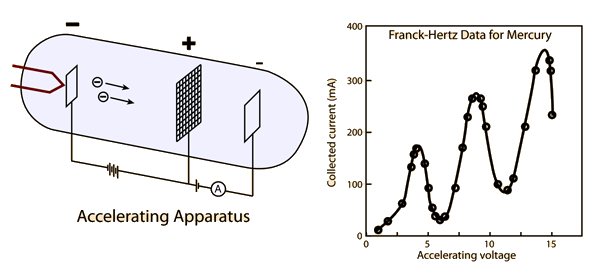
\includegraphics[width=\textwidth]{fotos/T1.5.Franck-Hertz.png}
    \end{wrapfigure}

    \noindent Conforme se aumenta el potencial, más electrones llegan a la placa que 
    registra y mayor la corriente. Se observa que a cierto valor de voltaje, baja: 
    tenemos el metal a estudiar en gas, y lo que ocurre esq tenemos T suficiente para 
    que los e saltasen. 

    \vspace{0.4cm} \noindent Por tanto, la energía que gana la pierde al pasar de un 
    estado 1 a 2, los electrones salen sin T y por haber potencial que los repele no 
    llegan a la placa. Con esto se demuestra la cuantización de los estados. 

  \section{Longitud de onda de De Broglie}
    \noindent Llegado a este punto entra De Broglie, que propone que no solo las ondas 
    se pueden comportar como corpúsculo, sino corpúsculo como onda.\\
    
    
    \noindent 
    \begin{equation}
      \begin{rcases}
        &\text{ENERGÍA}\\
        &\text{FOTÓN}
      \end{rcases}
      E=pc\hspace{0.3cm}E=h\nu=\dfrac{hc}{\lambda}\hspace{0.2cm}\implies\hspace{0.2cm}
      \dfrac{hc}{\lambda}=pc\hspace{1cm}\boxed{\lambda=\dfrac{h}{p}}
      \label{eq:deBroglie}
    \end{equation}

    \vspace{0.4cm}
    \noindent Propuso que las partículas se pueden comportar como ondas y que su 
    longitud de onda viene determinada por su momento lineas (y por ello su velocidad).

    \vspace{0.8cm}
    \noindent Nos queda ver cómo los postulados de Bohr solucionan el hecho de que las 
    órbitas de los electrones no irradian.

    \noindent $L_n=n\hbar\hspace{1cm}mrv=n\hbar\hspace{1cm}2\pi r(mv)=nh
    \xRightarrow{\ref{eq:deBroglie}}2\pi r \cdot \dfrac{h}{\lambda}=nh
    \hspace{1cm}\boxed{2\pi r =n\lambda}$ 
    \hspace{0.6cm} \textit{(la $\lambda$ es proporcional a $r$).}

    \vspace{0.8cm}
    \noindent Podemos decir que la onda que forma el electron es \textbf{estacionaria} 
    (el origen y final están quietos, si los unimos la onda es circular).

    \noindent \[\text{VECTOR DE ONDA}\hspace{0.2cm} \rightarrow \hspace{1cm} k=
    \dfrac{2\pi}{\lambda}<   \hspace{1cm}\vec{k}=[\vec{k}]=\dfrac{2\pi}
    {\lambda}\]

\clearpage

  \section{Ondas Clásicas}
    \noindent Vamos a trabajar con una onda sinusoidal de longitud de onda $\lambda$, 
    periodo $T$ y fase inicial en una única dimensión. Las expresiones que describen 
    este movimiento son las siguientes:

    \begin{equation}
      y(x,t)=y_0\cos\left(kx\pm \omega t+\varphi_0\right) \hspace{0.4cm} 
      \text{CONVENIO DE SIGNOS: <\ 0 mueve hacia la derecha}
    \end{equation}

    \vspace{0.15cm}
    \teorema{}{
      \def\arraystretch{2}
      \begin{tabular}{lll}
        &Número de onda: &$k=\dfrac{2\pi}{\lambda}$\\
        &Frecuencia angular: &$\omega=2\pi\nu=\dfrac{2\pi}{T}$\\
        &Velocidad/fase de propagación: &$v_f=\lambda\nu=\dfrac{\omega}{k}$
      \end{tabular}
    }

    \noindent Se puede comprobar que la expresión dada cumple la ecuación de onda, 
    lo cual una vez aplicado De Broglie implica que el momento $p$ está bien definido:

    \begin{equation}
      \text{ECUACIÓN DE ONDA}\hspace{1cm} \dfrac{\partial^2y}{\partial x^2}=\dfrac{1}{v_f^2}\cdot
      \dfrac{\partial y^2}{\partial t^2}
    \end{equation}
    
    \noindent Aquí hallamos el principio de incertidumbre de Heisemberg, puesto que 
    conocemos su momento lineal $p$ pero no su posición, ergo la onda está 
    deslocalizada.

    \definicion{Onda plana}{
      Llamamos onda plana a aquella onda cuyo frente de onda se ve en un plano.

      \begin{wrapfigure}[9]{l}{.23\textwidth}
        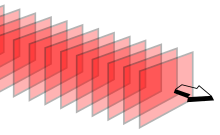
\includegraphics[width=\textwidth]{fotos/ondaPlana.png}
      \end{wrapfigure}
      $$y(x,t)=a_0e^{i(kx\pm\omega t)}\hspace{1cm}a_0=y_0e^{il_0}$$
      Está expresada en forma compleja (notación que usaremos de ahora en adelante,
      puesto que la parte cqmpleja cobra sentido físico en la mecánica cuántica), y 
      para obtener la onda clásica nos quedamos solo con la parte real:
      $$Re\left[y(x,t)\right]=Re\left[y_0 e^{kx\pm\omega t+l_0}\right]=y_0\cos
      (kx\pm\omega t+l_0)$$
    }
    \teorema{Principio de superposición}{
      Si $y_1$ e $y_2$ son soluciones de la ecuación de onda, una combinación lineal
      de ellas también lo será.
    }
    \definicion{Ondas estacionarias}{
      \begin{wrapfigure}[5]{l}{.23\textwidth}
        \vspace{-0.5cm}
        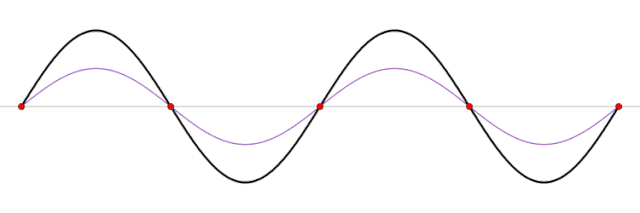
\includegraphics[width=\textwidth]{fotos/nodos.png}
      \end{wrapfigure}

      Se llama onnda estacionaria a aquella onda cuyos nodos permanecen inmóviles.
      Llamamos nodos a los puntos de la onda cruzan el eje de abcisas y son por tanto
      estáticos en las ondas estacionarias.
    } 
    \teorema{Interferencia de una onda consigo misma}{
      \begin{itemize}
        \item Hacia la derecha:$\hspace{0.35cm}y_1=y_0\sin(kx-\omega t)$
        \item Hacia la izquierda: $y_2=y_0\sin(kx+\omega t)$
      \end{itemize}
    }

\clearpage

    \noindent Para ver la onda resultante de la interferencia de ambas, las sumamos:
    $y=y_1+y_2=y_0\left[\sin(kx-\omega t)+\sin(kx+\omega t)\right]=2y_0\sin\left(
    \dfrac{kx-\omega t+kx+\omega t}{2}\right)\cdot\left(\dfrac{kx-\omega t-kx+\omega 
    t}{2}\right)\Leftrightarrow \boxed{y=2y_0\sin(kx)\cos(\omega t)}$\\ 
    \vspace{0.8cm} Sabiendo que $\sin\alpha+\sin\beta=2\sin\left(\dfrac{\alpha+\beta}{2}
    \right)\cdot\left(\dfrac{\alpha-\beta}{2}\right)$

    \noindent Ahora, aplicamos las condiciones de contorno:
    $t=0, y(x=L) \Longleftrightarrow \boxed{k\cdot L = n\pi\hspace{0.6cm}n=0,1,2...}$\\

    \noindent Donde cada valor de $n$ se le llama \textbf{armónico}. Esta relación 
    puede cambiar si se dan condiciones de contorno distintas.\\
      
    \noindent Como $k=\dfrac{2\pi}{\lambda}$ y $\dfrac{2\pi}{\lambda}\cdot L=n\pi$
    entonces, $\boxed{\lambda=\dfrac{2\pi}{n}}$
    
    \vspace{0.4cm}
    \definicion{Paquete de ondas}{
      Llamamos \textbf{paquete de ondas} a un conjunto de ondas sinusoidales de igual 
      amplitud pero distinta longitud de onda y frecuencia.

      $$\begin{rcases}
        &y_1=A\cos(k_1x-\omega_1 t)\\
        &y_2=A\cos(k_2x-\omega_2 t)
      \end{rcases}$$

      \begin{align}
        \begin{split}
          y(x,y)=y_1+y_2=A\left[\cos(k_1x-\omega_1 t)+\cos(k_2x -\omega_2 t)\right]=\\
          2A\cos\left(\dfrac{k_1+k_2}{2}x-\dfrac{\omega_1+\omega_2}{2}t\right)\cos\left(
          \dfrac{k_1-k_2}{2}x-\dfrac{\omega_1-\omega_2}{2}t\right)
          \label{eq:paqueteDeOndas}
        \end{split}
      \end{align}

      \noindent Siendo los \textbf{valores medios}: $\langle k\rangle=\dfrac{k_1+k_2}
      {2},\hspace{0.6cm}\langle w\rangle=\dfrac{\omega_1+\omega_2}{2}$

      \vspace{0.4cm} \noindent Cada onda se mueve con velocidad $v_1 = \dfrac{\omega_1}{k_1}$ y 
      $v_2 = \dfrac{\omega_2}{k_2}$ respectivamente. Además, podemos calcular la 
      velocidad de fase con los valoores medios que acabamos de definir:
      \[v_f=\dfrac{\langle\omega\rangle}{\langle k\rangle}\]

      \noindent También podemos calcular la velocidad de grupo, que es la velocidad a
      la que se mueve el paquete de ondas:
      \[v_g=\dfrac{\Delta\omega}{\Delta k}\]

      \noindent Cuando hacemos una superposición sí que podemos localizar la partícula,
      pero perdemos información sobre su momento. Esto nos vuelve a llevar otra vez
      al principio de incertidumbre de Heisemberg.
    }

\clearpage

    \ejemplo{Consideramos las siguientes tres ondas y calculamos la superposición de su
    interferencia (sumándolas)}{
      \begin{equation*}
        \begin{rcases}
          \psi_1(x)=\psi_0 e^{ik_0x}\\
          \psi_2(x)=\frac12\psi_0e^{i\left(k_0-\frac{\Delta k}{2}\right)x}\\
          \psi_3(x)=\frac12\psi_0e^{i\left(k_0+\frac{\Delta k}{2}\right)x}
        \end{rcases}
        \psi(x)=\psi_0e^{ix_0x}\left(1+\frac12 e^{-i\frac{\Delta k}{2}x}+
        \frac12 e^{i\frac{\Delta k}{2}x}\right) \Rightarrow 
        \begin{rcases}
          e^{i\theta}=\cos\theta + i\sin\theta\\
          e^{-i\theta}=\cos\theta - i\sin\theta
        \end{rcases}
        2\cos\theta =e^{i\theta}+e^{-i\theta}
      \end{equation*}

      \[\boxed{\psi(x)=\psi_0e^{ik_0x}\left(1+\cos\left(\dfrac{\Delta k}{2}x\right)
      \right)}\]

      \noindent En los extremos tenemos que la función se anula y en el centro, que 
      tiene un máximo. Se dice que la onda está localizada y tiene anchura $\Delta x$.

      \noindent La representación de una partícula se puede dar como un paquete de
      ondas, donde se sabe que la partícula está en $\Delta x$ (relación con 
      Schrödinger porue perdemos informacińo sobre el momento).

      \noindent Podemos construir un paquete de ondas sumando tantas ondas como queramos.
      Una suma infinita de ondas planas con distintios valores de número de onda o de 
      momento se denomina \textit{Serie de Fourier}.
    }
    \definicion{Series de Fourier}{
      Cualquier función periódica se puede escribir como suma de senos y cosenos.
      \begin{equation}
        \psi(x)=\sum_{n=1}^{\infty}A_ne^{ik_n x}
        \label{eq:SerieFourier}
      \end{equation}
      Donde $A_n$ son las amplitudos de las ondas, el peso que cada onda tiene 
      en la función.
    }
    \noindent Vamos a ver que $k$ puede tomar cualquier valor continuo no discreto:
    \begin{equation}
      k\text{ continua}\implies \boxed{\psi(x)=\dfrac{1}{\sqrt{2\pi}}\int g(k)e^
      {ikx}\ dk}
      \label{eq:SerieFourierContinuo}
    \end{equation}
    \noindent $g(k)$ tiene el mismo papel que los coeficientes $A_n$ en el 
    caso discreto. $g(k)$ es la \textit{transformada de Fourier} de $\psi(x)$.
    \teorema{Plancherel}{
      \begin{equation}
        g(k)=\dfrac{1}{\sqrt{2\pi}}\int_{-\infty}^{+\infty}\psi(x)e^{-ikx}\ dx
        \label{eq:TeoremaPlancehrel}
      \end{equation}
      El valor de k estará relacionado con la energía de la partícula, será continua
      en el caso de una partícula libre (puesto que no tiene ningún tipo de 
      restricción). Si quiero hacer un paquete de onda para esa partícula libre, se 
      ha de hacer una integral.
    }
    \noindent Hemos definido dos velocidades distintas para los paquetes de ondas, 
    una velocidad de fase $v_f$ (ondas dentro del paquete) y una de grupo $v_g$ (de 
    todo el paquete). ¿Cómo las calculamos si tenemos un caso donde $k$ es continuo?

    \begin{itemize}
      \item Velocidad de grupo: $v_g=\dfrac{\Delta\omega}{\Delta k}\xrightarrow{k 
            \text{ continua}}v_g=\dfrac{d\omega}{dk}$\\ 
            
            \vspace{-0.2cm}A esta relación entre $\omega$ y $k$ se le llama \textbf{Relación 
            de dispersión}.
      \item Relación entre la velocidad de grupo y la velocidad de fase:\\
            $v_f=\dfrac{\omega}{k},\hspace{0.6cm}\omega=v_f\cdot k\Rightarrow v_g=
            \dfrac{d\omega}{dk}=\dfrac{d(v_f\cdot k)}{dk}=v_f+k\cdot\dfrac{dv_f}{dk}
            \Rightarrow\boxed{v_g=v_f+k\cdot\dfrac{dv_f}{dk}}$\\

            \vspace{-0.2cm}Si $v_f$ no varía, la onda no cambia de forma, pero si varía, se le  
            llamará \textbf{Onda Dispersiva}.
    \end{itemize}
  \section{Difriacción, doble rendija de Young}
    \begin{wrapfigure}[7]{l}{.3\textwidth}
      \vspace{-0.6cm}
      \includegraphics[width=\textwidth]{fotos/difracción.png}
    \end{wrapfigure}
    \noindent Dos rendijas separadas una distancia $d$ y una pantalla a una distancia $D$ tal
    que $D\textgreater\textgreater d$. Cuando se llega a la doble rendija, se producen nuevas ondas que interfieren
    entre ellas. Se espera encontrar un patrón de interferencia. Para que se produzca un 
    máximo, la diferencia de caminos debe ser un múltiplo de la longitud de onda $\lambda$.
    \[\Delta x=x_2-x_1=n\lambda\hspace{1cm}n\in\bbZ\]

    \noindent Vamos a ver la distancia entre dos máximos $\Delta y$ en función de algún dato
    que nos sea conocido.

    \noindent $\Delta x = d\cdot\sin\theta\Rightarrow$ Condición máximo: $\boxed{d\cdot\sin
    \theta=n\lambda}$ \hspace{1.5cm} $\dfrac{\Delta y}{D}=\tan\theta\simeq\sin\theta,\hspace{1cm}
    \boxed{\Delta y=\dfrac{n\lambda D}{d}}$\\

    \vspace{0.4cm}\noindent Vamos a estudiar cómo se presenta el patrón de interferencia:
    \begin{align}
      \begin{split}
        \text{Intensidad }\propto \abs{\psi}^2\Rightarrow\\
        \begin{rcases}
          \psi_1=\psi_0e^{i(kx_1-\omega t)}\\
          \psi_2=\psi_0e^{i(kx_2-\omega t)}
        \end{rcases}
        \Rightarrow\abs{\psi}^2=(\psi_1+\psi_2)\cdot(\psi_1+\psi_2)=\psi_1\cdot\psi_1+\psi_2\cdot
        \psi_2+\psi_1\cdot\psi_2+\psi_2\cdot\psi_1=\\ \abs{\psi_0}^2\left(e^{-i(kx_1-\omega t)}\cdot
        e^{i(kx_1-\omega t)}+e^{-i(kx_2-\omega t)}\cdot e^{i(kx_2-\omega t)}+e^{-i(kx_1-\omega t)}
        \cdot e^{i(kx_2-\omega t)}+e^{-i(kx_2-\omega t)}\cdot e^{i(kx_1-\omega t)}\right)=\\ \abs{
        \psi_0}^2e^{-i\omega t}\cdot e^{i\omega t}\left(2+e^{ik}(x_2-x_1)+e^{ik(x_1-x_2)}\right)=\\
        \abs{\psi_0}^2\left(2+e^{ik\Delta x}+e^{-ik\Delta x}\right)=\\ \abs{\psi_0}^2\left(
        2+2\cos(k\Delta x)\right)=\\ \abs{\psi_0}^2\cdot 4\cos^2\left(\dfrac{k\Delta x}{2}\right)
      \end{split}
    \end{align}
    \noindent Sabiendo que por Euler $e^{ik\Delta x}+e^{-ik\Delta x}=2\cos(k\Delta x)$ y que 
    $\cos(2\theta)+1=2\cos^2\theta$

    \noindent En conclusión, la función que se observa en el patrón:
    \begin{equation}
      \boxed{\abs{\psi_0}^2\cdot4\cos^2\left(\dfrac{k\Delta x}{2}\right)}
      \label{eq:PatronInterferencia}
    \end{equation}

    \noindent ¿Por qué aparece este patrón de interferencia y no solo partículas por donde pasan
    los electrones? Por los \textbf{términos de interferencia}, que no se cancelan (si lo 
    hicieran, tendríamos únicamente dos bandas por donde pasan los rayos).
\chapter{La ecuación de Schrödinger I}
  \section{Mecánica clásica no relativista en una dimensión}
    \noindent Clásicamente, se han usado las ecuaciones de Newton para describir la dinámica.
    % \begin{align}
    %   \begin{split}
    %     &F=m\cdot a\\
    %     &\text{Fuerzas conservativas }\rightarrow F=-\dfrac{\partial U}{\partial x}\\
    %     &m\dfrac{d^2x}{d^t}=-\dfrac{\partial U}{\partial x}\\
    %   \end{split}
    % \end{align}
    En la mecánica cuántica, usaremos una función llamada 'onda de materia' denotada
    $\Psi(x,t)$, donde nos interesa estudiar la evolución temporal de esta onda. Esta ecuación
    es un postulado, no se deriva de otras. Schrödinger propuso esta ecuación y la utilizamos
    porque funciona, los resultados experimentales se corresponden con el artefacto matemático
    que Schrödinger propuso. Podemos sin embargo tratar de motivar la idea que siguió para definir 
    la ecuación de una forma concreta.\\

    \definicion{Ecuación de Schrödinger}{
      \begin{equation}
        i\hbar \dfrac{\partial\Psi}{\partial t}=-\dfrac{\hbar^2}{2m}\dfrac{\partial^2\Psi}
        {\partial x^2}+U\cdot\Psi
      \end{equation}
    }

    \noindent Supongamos una onda de materia del tipo onda plana: $\Psi(x,t)=\Psi_0\cdot e^{i(kx-\omega t)}$.
    Vamos a reescribir el número de onda y la frecuencia como múltiplos de $\hbar^{-1}$

    \begin{equation}
      \begin{rcases}
        &k=\dfrac{2\pi}{\lambda}\\
        &\lambda= \dfrac{h}{p}
      \end{rcases} \rightarrow k=\dfrac{2\pi p}{h}=\dfrac{p}{\hbar}
      \hspace{2cm}
      \begin{rcases}
        &\omega=2\pi\nu\\
        &E=h\nu
      \end{rcases}\rightarrow\omega=\dfrac{2\pi}{h}E=\dfrac{E}{\hbar}
    \end{equation}

    \noindent Así, podemos reescribir la ecuación de onda plana como:

    \begin{equation}
      \Psi(x,t)=\Psi_0\cdot e^{\frac{i}{\hbar}(px-Et)}
    \end{equation}

    \noindent La energía cinética de una partícula libre en función del momento lineal
     es $E=\dfrac{p^2}{2m}$

    \noindent Si derivamos esta ecuación en función del tiempo y la posición obnetemos:
    \[\dfrac{\partial\Psi}{\partial t}= \dfrac{-i}{\hbar}E\cdot\Psi\rightarrow E=-\dfrac{\hbar}{i}
    \dfrac{1}{\Psi}\dfrac{\partial\Psi}{\partial t}\]
    \[\dfrac{\partial\Psi}{\partial x}=\dfrac{i}{\hbar}p\Psi\]
    \[\dfrac{\partial^2\Psi}{\partial x^2}=-\dfrac{p^2}{\hbar^2}\Psi\rightarrow p^2=-\dfrac{\hbar^2}
    {\Psi}\dfrac{\partial^2 \Psi}{\partial x^2}\]

    \begin{equation}
      i\hbar\dfrac{1}{\Psi}\dfrac{\partial\Psi}{\partial t}=-\dfrac{-h^2}{2m}\dfrac{1}{\Psi}
      \dfrac{\partial^2\Psi}{\partial x^2}\Longrightarrow\boxed{i\hbar\dfrac{\partial\Psi}{\partial t}=
      -\dfrac{\hbar^2}{2m}\dfrac{\partial^2\Psi}{\partial x^2}}
      \label{eq:SchrodingerParticulaLibre}
    \end{equation}

    \noindent Podemos reescribir esta ecuación en términos del hamiltoniano ya que la primera 
    parte de la ecuación describe la energía total, el primer término de la segunda parte la energía
    cinética, y el último la potencial. El hamiltoniano en mecánica clásica es 
    $H(x,t)=\dfrac{p^2}{2m}+U$.

    \definicion{Operadores}{
      \subsubsection*{Operador momento}
      \begin{equation}
        \hat{p} = -i\hbar\dfrac{\partial}{\partial x}
      \end{equation}
      \subsubsection*{Operador posición}
      \begin{equation}
        \hat{x} = x
      \end{equation}
      \subsubsection*{Operador hamiltoniano}
      \noindent Para el caso del hamiltoniano, vemos como la única diferencia entre el 
      hamiltoniano clásico y el operador hamiltoniano son los operadores.
      \begin{equation}
        \hat{H}(x,t)=\dfrac{\hat{p}^2}{2m}+U(\hat{x})\ \Longrightarrow\ \hat{H} = -\dfrac{\hbar^2}{2m}
        \dfrac{\partial^2}{\partial x^2} + U(x)
      \end{equation}
      \subsubsection*{Operador energía}
      \begin{equation}
        \hat{E} = i\hbar\dfrac{\partial}{\partial t}
      \end{equation}
    }

    \noindent Si le aplicamos el operador hamiltoniano y energía a la función de onda:\\
    \[\hat{H}\Psi=-\dfrac{\hbar^2}{2m}\dfrac{\partial^2\Psi}{\partial x^2}+U\Psi\]
    \[\hat{E}\Psi=i\hbar\dfrac{\partial\Psi}{\partial t}\]

    \begin{equation}
      \boxed{\hat{E}\Psi=\hat{H}\Psi}
      \label{eq:autoEnergiaHamiltoniano}
    \end{equation}

    \comentario{Comprobar que una función real no cumple la ecuación de Schrödinger, por ejemplo
    $\Psi(x,t)=\Psi_0\cos(kx-\omega t)$ (y tampoco una imaginaria pura).}

  \section{Interpretación de la función de onda}
    \noindent La llamada \textit{interpretación de Copenhague} fue aquella postulada por Max Born, 
    quien propuso que el significado físico no lo portaba la función de onda, si no su cuadrado: 
    $\abs{\Psi(x,t)}^2\cdot dx$. Y esto no es más que una probabilidad, la probabilidad de que la 
    partícula se en cuentre entre $x$, y $x+dx$. Intrínsicamente no podemos conocer con certeza la 
    posición, a diferencia de en la mecánica estadística, en la que la probabilidad viene de la 
    imposibilidad de medida de todo el sistema. \\

    \definicion{Densidad de probabilidad}{
      \begin{equation}
        \mcP(x,t)=\abs{\Psi(x,t)}^2
      \end{equation}
    }
    \comentario{
      Unidades de la función de onda: $[\Psi]=\dfrac{1}{[\sqrt{L}]}$
    }
    
\clearpage

    \noindent Para conocer la probabilidad de que una partícula se encuentre entre dos puntos $x=a$ 
    y $x=b$, no hay más que integrar: 
    \begin{equation}
      \mcP_{[a,b]}=\int_a^b\abs{\Psi(x,t)}^2\ dx
      \label{eq:densidaddeprobabilidad}
    \end{equation}

    \noindent Vemos como para que esto tenga sentido y la función de onda represente a una partícula, 
    la integral sobre todo el rango de definición debe ser 1, es decir, que la función de onda debe 
    estar normalizada: 
    \begin{equation}
      \int_{\infty}^\infty\abs{\Psi(x,t)}^2\ dx=1
    \end{equation}

    \noindent Si hacemos un a medida y encontramos que la partícula se encuentra en $x=A$, Einstein
    nos diría que la partícula se encontraba ya ahí anteriormente, y Bohr diría que la partícula se
    encontraba en una superposición de todas las posiciones posibles, y al realizar la medida 
    definimos su posición. Lo que llamamos el colapso de la función de onda.\\

    \noindent Después de la primera medida la función de onda pasa a ser similar a una delta de Dirac
    centrada en el punto $x=A$.

    \teorema{Propiedades de la función de onda $\Psi(x,t)$ para que esta represente una partícula}{
      \begin{itemize}
        \item Debe ser compleja
        \item Debe estar normalizada $\int_\infty^\infty\abs{\Psi(x,t)}^2\ dx=1$ (para que 
              una función sea normalizable, los límites en el infinito deben ser 0).\hspace{0.6cm}
              $\lim_{(x\rightarrow\infty,t)}\Psi(x,t)=0$\hspace{0.6cm}
              $\lim_{(x\rightarrow-\infty,t)}\Psi(x,t)=0$
        \item Debe ser una función continua y unievaluada.
        \item Si $\Psi_1$ y $\Psi_2$ son soluciones de la \textit{Ecuación de Schrödinger}, 
              una combinación lineal de ellas tamibén es solución. (Principio de superposición)
              $\Phi(x,t)=\alpha\Phi_1+\beta\Phi_2$.\\
              Si conozco la condición inicial de la función de onda, conocemos la evolución temporal,
              es decir, es una ecuación determinística. $\Psi(x,t=0)\implies\abs{\Psi(x,t)}^2$
      \end{itemize}
    }
    
  \section{Ecuación de continuidad}
    \noindent Vamos a ver que se cumple una ecuación de continuidad análoga a la de la conservación 
    de carga en \textit{Electromagnetismo}, o la que se ve en \textit{Mecánica de fluidos}.

    \definicion{Ecuación de continuidad}{
      Una vez hemos definido la densidad de probabilidad \ref{eq:densidaddeprobabilidad}, vamos a 
      estudiar cómo varía esta función en el tiempo, es decir, su derivada temporal.\\ 
      
      $\text{Conociendo que: }
      \begin{rcases}
        i\hbar\dfrac{\partial\Psi}{\partial t}=-\dfrac{\hbar^2}{2m}\dfrac{\partial^2\Psi}{\partial x^2}+U\Psi\\
        -i\hbar\dfrac{\partial\Psi^*}{\partial t}=-\dfrac{\hbar^2}{2m}\dfrac{\partial^2\Psi^*}{\partial x^2}+U\Psi^*
      \end{rcases}$\\

      \vspace{0.4cm}$\dfrac{\partial\mcP(x,t)}{\partial t}=\dfrac{\partial}{\partial t}\left(\Psi^*\cdot\Psi\right)=
      \dfrac{\partial\Psi^*}{\partial t}\Psi +\dfrac{\partial\Psi}{\partial t}\Psi^*$
      $=\left(\dfrac{\hbar}{i2m}\dfrac{\partial^2 \Psi^*}{\partial x^2}-\dfrac{U}{i\hbar}\Psi^*\right)\Psi +
      \left(-\dfrac{\hbar}{i2m}\dfrac{\partial^2 \Psi}{\partial x^2}+\dfrac{U}{i\hbar}\Psi\right)\Psi^* =
      \left(-\dfrac{i\hbar}{2m}\dfrac{\partial^2 \Psi^*}{\partial x^2}\Psi+ \dfrac{i\hbar}{2m}\dfrac{\partial^2 \Psi}{\partial x^2}\Psi^*\right)=
      \dfrac{i\hbar}{2m}\left(\dfrac{\partial^2}{\partial x^2}\Psi^*-\dfrac{\partial^2\Psi^*}{\partial x^2}\Psi\right)=
      $
      $\dfrac{i\hbar}{2m}\dfrac{\partial}{\partial x}\left(\dfrac{\partial \Psi}{\partial x}\Psi^*-\dfrac{\partial \Psi^*}{\partial x}\Psi\right)$
      
      \vspace{0.4cm}
      ($\dfrac{\partial}{\partial x}\left(\dfrac{\partial\Psi}{\partial x}\Psi^*-\dfrac{\partial\Psi^*}{\partial x}\Psi\right)=
      \dfrac{\partial^2\Psi}{\partial x^2}\Psi^*+\dfrac{\partial\Psi}{\partial x}\dfrac{\partial\Psi^*}{\partial x}-
      \dfrac{\partial^2\Psi^*}{\partial x^2}\Psi-\dfrac{\partial\Psi^*}{\partial x}\dfrac{\partial\Psi}{\partial x}$)
    }
    \definicion{Corriente de probabilidad}{
      Una ecuación de continuidad es una ecuación que nos dice que hay una conservación de algún tipo, 
      en nuestro caso lo que se conserva es la probabilidad.

      \begin{equation}
        \mcJ(x,t)=\dfrac{i\hbar}{2m}\left(\Psi\dfrac{\partial\Psi^*}{\partial x}-\Psi^*\dfrac{\partial \Psi}
      {\partial x}\right) \implies \boxed{\dfrac{\partial\mcP(x,t)}{\partial t}=-\dfrac{\partial\mcJ(x,t)}{\partial x}}
      \label{eq:corrienteProbabilidad}
      \end{equation}

      \noindent Reescrito:
      $\dfrac{\partial\mcP(x,t)}{\partial t}+\dfrac{\partial\mcJ(x,t)}{\partial x}=0$
    }

    \noindent Una vez tenga la función de onda normalizada, lo estará de forma independiente del tiempo:
    Si integramos sobre todo el espacio: 
    \[\int_{-\infty}^{\infty}\dfrac{\partial\mcP(x,t)}{\partial t}\ dx+\int_{-\infty}^{\infty}\dfrac{\partial\mcJ(x,t)}{\partial x}\ dx=0\]
    \[\dfrac{\partial}{\partial t}\int_{-\infty}^{\infty}\mcP(x,t)\ dx+\mcJ_(x=0,t)-\mcJ(x=0,t)=0\] 

    \noindent En conclusión, si $\Psi(x,t)$ es normalizable, lo estará para cualquier tiempo.
    \begin{equation}
      \dfrac{\partial}{\partial t}\int_{-\infty}^{\infty}\mcP(x,t)\ dx=0
    \end{equation}
  \section{Valores esperados y observables}
    \noindent Llamamos valor observable a cualquier magnitud susceptible de medida.
    Todo parámetro observable va a estar relacionado con un operador y viceversa. Nos gugstaría conocer,
    por ejemplo, cuál sería el valor esperado dela posición de la partícula, que denotaremos por $\langle x\rangle$.\\

    \noindent Esta probabilidad en un caso discreto es $\langle x\rangle=\sum x_n\cdot P_n$.
    En el caso continuo: $\langle x\rangle=\int x\cdot f(x)\ dx$ donde $f(x)$ es una función de probabilidad.
    Sabemos que en cuántica esto es el cuadrado de la función de onda:
    \begin{equation}
      \int_{-\infty}^{\infty}x\abs{\Psi(x,t)}^2\ dx=\int_{-\infty}^{\infty}\Psi^*\times\Psi\ dx
    \end{equation}

    \noindent Calcular un valor medio no implica volver a medir la misma posición sobre la misma partícula 
    (puesto que colapsa y volvería a $x_a$), sino que tendríamos que preparar 
    varias partículas con la misma función de probabilidad, hacerlas colapsar y tomar el valor 
    esperado de la posición respecto a la medida que vayamos a tomar de cada una.\\

    \noindent Esta definición es extedible a cualquier valor observable $Q$: $Q\rightarrow\langle Q\rangle=
    \int_{-\infty}^{\infty}Q\cdot\abs{\Psi(x,t)}^2\ dx$

    \noindent Vamos a ver cómo cambiará el valor eseperado de un valor observable en el tiempo, su derivada temporal:
    \[\dfrac{d\langle x\rangle}{dt}=\dfrac{d}{dt}\int_{-\infty}^{\infty}x\abs{\Psi(x,t)}^2\ dx=
    \int_{-\infty}^{\infty}x\dfrac{\partial}{\partial t}\abs{\Psi(x,t)}^2\ dx=\int_{-\infty}^{\infty}
    x\dfrac{\partial}{\partial t}(\Psi^*\cdot\Psi)\ dx=\dfrac{i\hbar}{2m}\int_{-\infty}^{\infty}
    x\dfrac{\partial}{\partial x}\left(\Psi^*\dfrac{\partial\Psi}{\partial x}-\dfrac{\partial\Psi^*}{\partial x}\Psi\right)\ dx\]

    \noindent Resolviendo por partes:\\ 
    \[\int_{-\infty}^{\infty}x\dfrac{\partial}{\partial x}\left(\Psi^*\dfrac{\partial\Psi}{\partial x}\ dx\right)=
    -\int_{-\infty}^{\infty}\Psi^*\dfrac{\partial\Psi}{\partial x}\ dx+x\Psi^*\dfrac{\partial\Psi}{\partial x}\Big|_{-\infty}^{+\infty}\]
    \noindent \textit{Idem} con la segunda parte.\\

\clearpage
    \noindent En conclusión:
    \begin{equation}
      \dfrac{d\langle x\rangle}{dt}=\dfrac{i\hbar}{2m}\int_{-\infty}^{\infty}\left(\dfrac{\partial\Psi^*}{\partial x}\Psi-\Psi^*\dfrac{\partial\Psi}{\partial x}\right)\ dx \implies
      \boxed{\dfrac{d\langle x\rangle}{dt}=-\dfrac{i\hbar}{m}\int_{-\infty}^{\infty}\Psi^*\dfrac{\partial\Psi}{\partial x}\ dx}
    \end{equation}
    \[\implies \langle p\rangle=m\dfrac{d\langle x\rangle}{dt}=-i\hbar\int_{-\infty}^{\infty}\Psi^*\dfrac{\partial\Psi}{\partial x}\ dx=
    \int_{-\infty}^{\infty}\Psi^*\left(-i\hbar\dfrac{\partial}{\partial x}\Psi\ dx\right)\] 
    \[\implies \langle x\rangle=\int_{-\infty}^{\infty}\Psi^*\hat{x}\Psi\ dx=\int_{-\infty}^{\infty}\Psi^* x\Psi\ dx\]
    donde $-i\hbar\dfrac{\partial}{\partial x}\Psi$ es el operador momento lineal $\hat{p}$\\
    

    \noindent Generalizando el valor esperable:
    \begin{equation}
      \langle Q \rangle =\int_{-\infty}^{\infty}\Psi^*\hat{Q}\Psi\ dx
    \end{equation}

    \noindent En este caso necesitamos los operadores en el espacio de posiciones, 
    pero más adelante trabajaremos en el espacio de momentos y 
    cambiará la expresión de los operadores que ya hemos definido. A nivel práctico,
    tendríamos que hacre lo siguiente para cualquier magnitud que podamos 
    representar en función de $x$ ý $p$.\\

    \ejemplo{}{
      En mecánica clásica: $T=\dfrac{1}{2m}p^2$\\
      \[\langle T\rangle=\int_{\infty}^{\infty}\Psi^*\dfrac{1}{2m}\hat{p}^2\Psi\ dx=
      \int_{\infty}^{\infty}\Psi^*\left(-\dfrac{\hbar^2}{2m}\cdot\dfrac{\partial^2}
      {\partial x^2}\right)\Psi\ dx\]
    }

    \definicion{Incertidumbre}{
    La otra variable que nos interesa conocer a nivel probabilístico es la 
    desviación estándar, que sería equivalente a conocer la anchura de la Gaussiana. 
    Nos da la dispersión de los posibles valores. Es decir, la \textbf{incertidumbre}.
    \begin{equation}
      \sigma = \sqrt{\langle\Delta x^2\rangle}
    \end{equation}
    La dispersión de una variable observable $Q$, de valor esperado $\langle Q\rangle$
    la daremos de la siguiente forma:
    \begin{equation}
      \Delta Q^2=\left(Q-\langle Q\rangle\right)^2\hspace{0.5cm}\implies\hspace{0.5cm}
      \sigma=\sqrt{\langle\Delta Q^2\rangle}=\sqrt{\langle Q^2\rangle-\langle Q\rangle^2}
    \end{equation}
    Ya que: $\langle \Delta Q^2\rangle=\langle\left(Q-\langle Q\rangle\right)^2\rangle=
    \langle Q^2+\langle Q\rangle^2-2Q\langle Q\rangle\rangle=\langle Q^2\rangle-\langle Q
    \rangle^2$ (el valor esperado de la suma es la suma de valores esperados).\\

    Para sucesos independientes: $\langle Q\langle Q\rangle\rangle=\langle Q\rangle\cdot
    \langle Q\rangle$
    }
    \ejemplo{Suponemos que la función de onda que representa a una partícula tiene la
    siguiente forma:
    $\Psi\left(x,t=0\right)=\Psi_0\cdot e^{-\dfrac{(x-x_0)^2}{4\sigma x^2}}$}{
      Vemos como esta función es equivalente a una gaussiana centrada en $x_0$.

      \begin{enumerate}
        \item Normalizamos $\Psi\colon\displaystyle 
              \int_{-\infty}^{\infty}\abs{\Psi}^2\ dx= 1$\\
              
              $\displaystyle\int_{-\infty}^{\infty}\abs{\Psi_0}^2 e^{-
              \dfrac{2(x-x_0)^2}{4\sigma x^2}}\ dx=\abs{\Psi}^2
              \int_{-\infty}^{\infty}e^{-\dfrac{(x-x_0)^2}{2\sigma x}}\ dx=
              \abs{\Psi_0}^2\sqrt{2}\sigma x\int_{-\infty}^{\infty}e^{-y^2}\ dy
              =\abs{\Psi_0}^2\sqrt{2\pi}\sigma x=1$
              
              $\Longrightarrow \abs{\Psi_0}^2=
              \dfrac{1}{\sqrt{2\pi}\cdot\sigma_x}\Longrightarrow \Psi_0=\dfrac{1}
              {(2\pi\cdot\sigma_x^2)^{1/4}}$

        \item Tenemos un problema porque este número es real y debe ser complejo. Para
              solucionar esto, le asignamos una cierta fase:\\

              $\Psi_0=\dfrac{e^{i\varphi}}{(2\pi\cdot\sigma_x^2)^{1/4}}\hspace{0.3cm}\longrightarrow
              \hspace{0.3cm}\text{JUSTIFICACIÓN: }\abs{\Phi_0}^2=\Phi_0^2\cdot\Phi_0=
              \dfrac{e^{i\varphi}\cdot e^{-i\varphi}}{(2\pi\cdot\sigma_x^2)^{1/4}}=
              \dfrac{1}{\sqrt{2\pi}\sigma_x}$

              La probabilidad, que es lo que nos interesa por ser lo que tiene 
              significado físico, se mantiene igual. Por tanto, dos funciones de onda que 
              difieren en cierta fase representan el mismo objeto físico.

        \item Nos queda la siguiente función de onda: 
              $\Phi(x,t=0)=\dfrac{e^{i\varphi}}{(2\pi\cdot\sigma^2_x)^{1/4}}\cdot
              e^{-\dfrac{(x-x_0^2)}{4\sigma_x^2}}$\\
              Y calculamos ahora el valor esperado de $x$:\\
              $\langle x\rangle=\displaystyle\int_{-\infty}^{\infty}\Psi^*x\Psi\ dx=
              \int_{-\infty}^{\infty}\dfrac{e^{i\varphi}}{(2\pi\cdot\sigma_x^2)^{1/4}}
              \cdot e^{-\dfrac{(x-x_0)^2}{4\sigma_x^2}}\cdot x\cdot \dfrac{e^{i\varphi}}
              {(2\pi\cdot\sigma^2_x)^{1/4}}\cdot e^{-\dfrac{(x-x_0)^2}{4\sigma_x^2}}\ dx=
              \dfrac{1}{(2\pi\sigma_x^2)^{3/2}}\int_{\infty}^{\infty}x\cdot e^{-\dfrac{-(x-x_0)^2}
              {4\sigma_x}}\ dx=...=x_0$\\

              Esto tiene sentido por ser una gaussiana centrada en ese valor. También
              es posible comprobar que $\langle \Delta x^2\rangle=\sigma_x^2$. 
      \end{enumerate}
    }
\chapter{La ecuación de Schrödinger II}
  \noindent Hasta ahora hemos visto la ecuación de onda dependiente del tiempo, cuya 
  resolución es bastante complicada. Vamos a ver que esto se facilita con separación 
  de variables.\\
  \section{Estados estacionarios}
    \noindent Partimos de la siguiente ecuación, la \textit{Ecuación de Schrödinger} 
    dependiente del tiempo: (donde $\Psi=\Psi(x,t)$)\\
    \[i\hbar\dfrac{\partial\Psi}{\partial t}=-\dfrac{\hbar^2}{2m}\cdot
    \dfrac{\partial^2\Psi}{\partial x^2}+U\Psi\]

    \noindent La primera simplificación que haremos será considerar potenciales 
    independientes del tiempo $U=U(x)$. Puesto que una combinacińo lineal de soluciones
    también es solución, lo que haremos es proponer una solución y a partir de esta
    obtener el resto de soluciones (como las EDO de tipo Ricatti que vimos en 
    \textit{MAEDO}). En este caso, vamos a proponer una solución del siguiente tipo:
    \[\Psi(x,t)=\Psi(x)\cdot\varphi(t)\hspace{0.5cm}\text{con } 
    \varphi(t)=e^{\dfrac{-iEt}{\hbar}}\]

    

    \noindent Sustituimos esta expresión en la \textit{Ecuación de Shrödinger} y vemos
    que obtenemos:
    \[i\hbar\cdot\dfrac{\partial(\Psi\cdot\varphi)}{\partial t}=-\dfrac{\hbar^2}{2m}
    \cdot\dfrac{\partial^2(\Psi\cdot\varphi)}{\partial x^2}+U\Psi\varphi\]
    \[\Psi i\hbar\]

    \noindent Recordando la ecuación (\ref{eq:autoEnergiaHamiltoniano}), vemos como la función por el operador hamiltoniano
    es igual a un valor constante por la función. Este tipo de funciones las llamaremos
    \textit{autofunciones} (siempre van asociadas a un operador) y la constante (en este
    caso $E$) contiene a los \textit{autovalores}\\

    \noindent En los estados estacionarios la densidad de probabilidad es constante
    en el tiempo. 
    \[\langle H\rangle=\int_{-\infty}^{\infty}\Psi^*\hat{H}\Psi\ dx=
    \int_{-\infty}^{\infty}\Psi^*e^{i\frac{E}{\hbar}t}\hat{H}\Psi\ dx=
    \int_{-\infty}^{\infty}\Psi^*\hat{H}\Psi\ dx=
    \int_{-\infty}^{\infty}\Psi^* E\Psi\ dx=E\int_{-\infty}^{\infty}\Psi^*\Psi\ dx=E\]
    \[\boxed{\langle H\rangle=E\hspace{0.5cm}\text{ y }\hspace{0.5cm}
    \sigma_H=\sqrt{\langle H^2\rangle-\langle H\rangle^2}=0}\]

    \subsubsection{Solución general}
      \noindent Si conocemos los estados estacionarios (o las autofunciones $\Psi$ y autovalores 
      $E_n$ para el Hamiltoniano), la solución general será una combinación lineal de ellos:
      \[\Psi(x,t)=\sum_{n=1}^{\infty}c_n\cdot\Psi_n(x)\cdot e^{\frac{-iE_nt}{\hbar}}\]

      \noindent Definimos $\abs{c_n}^2$ como la probabilidad de que al medir la energía de ese
      sistema obtenga el valor de $E_n$.

      \ejemplo{Si tenemos dos estados (autofunciones) $\Psi_1(x)$ $\Psi_2(x)$ con energías
      $E_1$ y $E_2$ vamos a calcular la densidad de probabilidad y la solución general}{
      
        $\Psi(x,t)=c_1\Psi_1(x,t)e^{\frac{-iE_1}{\hbar}}t+c_2\Psi_2(x,t)e^{\frac{-iE_2}{\hbar}}t$\\
        $\abs{\Psi(x,t)}^2=c_1^2\Psi_1^2+c_2^2\Psi_2^2+c_1c_2\Psi_1\Psi_2
        \left(e^{\frac{-i\left(E_1-E_2\right)t}{\hbar}}+e^{\frac{i\left(E_1-E_2\right)t}
        {\hbar}}\right)$
      }

      \ejemplo{Suponemos una partícula de masa $m$ sometida a un potencial fijo: \\
          $V(x)=$
          $\begin{cases}
            0      & 0\leq x\leq a\\
            \infty &\text{para cualquier valor de } x
          \end{cases}$ 
        }{
          \vspace{-0.2cm}\subsubsection{Pozo de potencial cuadrado infinito}

          $\dfrac{-\hbar^2}{2m}\dfrac{d^2\psi}{dx^2}+U\psi= E\psi \Longleftrightarrow
          \dfrac{-\hbar^2}{2m}\dfrac{d^2\psi}{dx^2}=E\psi \longrightarrow 
          \dfrac{d^2\psi}{dx^2}=-\dfrac{2mE}{\hbar}\psi$ y llamamos
          $k = \dfrac{\sqrt{2mE}}{\hbar}$\\

          \noindent Sabemos que $E>0$ para que la función sea normalizable, lo que nos lleva 
          a resolver la ecuación:
          \[\dfrac{d^2\psi}{dx^2}=-k^2\psi\]
          \noindent Propuestas a solución: 
          \begin{itemize}
            \item $\psi(x)=A\sin(kx)+B\cos(kx)$
            \item $\psi(x)=A^\prime e^{-ikx}+B^\prime e^{ikx}$
          \end{itemize}
          Vamos a usar la primera, por lo que hemos de dar las condiciones de contorno.
          \begin{enumerate}
            \item $\psi_1(x=0)=\psi_2(x=0) \Longleftrightarrow A\cdot\sin(k0)+B\cos(k0)=0 
                  \Longrightarrow \boxed{B=0}$ \\
            \item $\psi_2(x=a)=\psi_3(x=a)$ y como $\psi_2(x)=A\sin(kx) \longrightarrow
                  A\sin(ka)=0 \Longrightarrow \boxed{ka=n\pi}\text{ con }n=1,2,3...$ 
                  Sabiendo que $n$ no puede ser 0 porque si lo es entonces $k=0$ y por
                  tanto $E=0$ y $\psi=0$\\
  
                  Despejando ahora la energía sabiendo que $k=\dfrac{\sqrt{2mE}}{\hbar}$ y
                  $k=n\dfrac{\pi}{a}\Longrightarrow k^2\hbar^2=2mE\longrightarrow
                  E=\dfrac{k^2\hbar^2}{2m}\Longrightarrow$
                  \[\boxed{E_n=\dfrac{n^2\pi^2\hbar^2}{2ma^2}}\]
                  Que es nuestra condición de cuantización de la energía.
            \item $\int_{-\infty}^{\infty}\abs{\psi(x)}^2\ dx= 1\Longleftrightarrow 
                  \int_{0}^a\abs{A}^2\sin^2(kx)\ dx=1 \Longleftrightarrow \abs{A}^2=\dfrac{2}{a}
                  \longrightarrow \boxed{A=\sqrt{\dfrac{2}{a}}}$
          \end{enumerate}
          Finalmente, obtenemos nuestras autofunciones para el pozo infinico:
          $\boxed{\psi_n(x)=\sqrt{\dfrac{2}{a}}\sin\left(\dfrac{n\pi}{a}x\right)}$\\

          \noindent La solución general para un potencial $U(x)$ dadas unas condiciones
          iniciales $\Psi(x,0)$ conociendo $\psi_n$ y $E_n$:
          \[\Psi(x,t)=\sum_{n=1}^{\infty}c_n\psi_n e^{-i\dfrac{E_n}{\hbar}t}\]
          Donde vemos que solo nos falta conocer $c_n=\int_{-\infty}^{\infty}
          \psi_n^*\cdot\psi(x,0)\ dx$ para los cuales habremos de resolver la
          \textit{Ecuación de Schrödinger} independiente del tiempo. Otra forma
          de obtener los coeficientes es a través de la igualdad $\displaystyle
          \Psi(x,0)=\sum_{n=1}^{\infty}c_n\psi_n$

        }
      \comentario{
        \noindent Las funciones de esta famila son ortonormales, es decir
        que para $n\neq m$, $\displaystyle\int_{\infty}^{\infty}\psi_m^*\cdot\psi_n=0$\\
      }
      \ejemplo{Suponemos una partícula de masa $m$ en un sistema en el que $U=0$
               \hspace{0.3cm}$\forall x$
      }{
        \vspace{-0.2cm}\subsubsection{Pozo de potencial cuadrado finito}
        La ecuación de una onda $\Psi(x,t)=\psi(x)\varphi(t)$\\
        \[\Psi(x,t)=\left(Ae^{-ikx}+Be^{ikx}\right)\cdot e^{-i\omega t}
        \hspace{1cm}\text{con }\omega=\frac{E}{\hbar}\]
        

        En el caso clásico: $H=\dfrac{p^2}{2m}$\hspace{0.5cm}$E=\dfrac{1}{2}mv^2
        \longrightarrow v_{\text{clásica}}=\sqrt{\dfrac{2E}{m}}$\\

        En cuántica: $\hspace{0.85cm}\hat{H}=\dfrac{\hat{p}^2}{2m}$\hspace{0.5cm}$\hat{H}\psi=E\psi
        \ \longrightarrow\  \dfrac{-\hbar^2}{2m}\dfrac{d^2\psi}{dx^2}=E\psi
        \ \longrightarrow\  \dfrac{d^2\psi}{dx^2}=-\dfrac{2mE}{\hbar^2}\psi
        \ \longrightarrow\  \dfrac{d^2\psi}{dx^2}=-k^2\psi$\\

        \noindent Propuestas a solución: 
        \begin{itemize}
          \item $\psi(x)=A\sin(kx)+B\cos(kx)$
          \item $\psi(x)=A^\prime e^{-ikx}+B^\prime e^{ikx}$
        \end{itemize}

        Vamos a buscar una relación entre la energía y la velociad. Sabemos que: 
        $v=\lambda\nu=\dfrac{\omega}{k}$ y que $k^2=\dfrac{2mE}{\hbar^2}$ y 
        $E=\hbar\omega$.

        Finalmente: $v=\dfrac{\omega}{k}=\dfrac{E}{\hbar k}=\dfrac{E\hbar}{\hbar\sqrt{2mE}}
        \Longrightarrow \boxed{v_{\text{cuántica}}=\sqrt{\dfrac{E}{2m}}}$\\

        \vspace{0.6cm}Encontramos dos problemas:
        \begin{itemize}
        \item Observamos como $v_{\text{clásica}}=2\cdot v_{\text{cuántica}}$ lo cual es preocupante.\\

        \item La ecuación de una onda que se propaga hacia la derecha con una energía $E=\hbar\omega$
        es: $\Psi(x,t)=A e^{+ikx-i\omega t}$. Aquí tenemos el otro problema, esta 
        función no es normalizable.\\
        \end{itemize}

        Para que $\Psi(x,t)$ represente a una partícula, debe cumplir que 
        $\int_{-\infty}^{\infty}\abs{\Psi(x,t)}^2\ dx= 1$
        \[\int_{-\infty}^{\infty}\Psi^*\Psi\ dx=\int_{-\infty}^{\infty}\abs{A}^2\cdot 
        e^{ikx+i\omega t}\cdot e^{-ikx-i\omega t}\ dt=\abs{A}^2\int_{-\infty}^{\infty}\ dx=
        \abs{A}^2(\infty)\Longrightarrow\text{\textbf{No es normalizable}}\]

        Es por esto, que para obtener la solución general vamos a usar una integral en vez
        de un sumatorio: 
        \[\Psi(x,t)=\dfrac{1}{\sqrt{2\pi}}\int_{-\infty}^{\infty}\tilde{\psi}(k)\psi(x)
        \cdot e^{\dfrac{-iEt}{\hbar}}\ dk\]
        Donde $\dfrac{1}{\sqrt{2\pi}}$ sale de la Transformada de Fourier, de
        las funciones que usamos como coeficientes $\tilde{\psi}(k)$

        Para el problema de las velocidades, vamos a recordar algunas expresiones:
        $v_f=\frac{\omega}{k}$, $v_\text{grupo}=\frac{d\omega}{dk}=\frac{\hbar k}{m}, 
        \omega = \frac{\hbar k^2}{2m}, k^2=\frac{2mE}{\hbar^2}$, $E=\hbar\omega$,
        $k^2=\frac{2m\hbar\omega}{\hbar^2}$ $\implies v_g=2\cdot v_f$\\

        Es decir, que la velocidad que se asemeja a la clásica es la velocidad de grupo.
        Con esto solucionamos el problema de las velocidades.
      }
      \ejemplo{Barreras y pozos de potencial finitos
        }{
        % \vspace{-0.2cm}\subsubsection{Barreras y pozos de potencial finitos}
        % %pedir foto
        % Vamos a resolverlo para dos casos, cuando $E>-V_0$ y $E<0$ con $-V_0<E<0$ y cuando
        % $E>0$.

        Encontraremos dos coeficientes para conocer información acerca de su transmisión $T$ y
        reflexión $R$.
        
        \subsubsection*{Estados ligados}
          \vspace{-0.2cm}Un estado ligado es aquel en el que $-V_0<E<0$
          $V(x)=$
          $\begin{cases}
            -V_0      & -a\leq x\leq a\\
              0       &\text{para cualquier otro valor de } x
          \end{cases}$ 

          Para resolverlo, vamos a definir tres regiones $I$, $II$ y $III$, una desde
          $-\infty$ hasta $-a$, otra desde $-a$ hasta $a$ y la última desde $a$ hasta $\infty$
          Como es un estado estacionario, sólo tenemos en cuenta el término de la posición:
          \begin{enumerate}
            \item $\dfrac{-\hbar^2}{2m}\dfrac{d^2\psi_I}{dx^2}=-\abs{E}\psi_I\Longleftrightarrow$
                  $\dfrac{d^2\psi_I}{dx^2}=\dfrac{2m\abs{E}}{\hbar^2}\psi_I$ que con $k=
                  \dfrac{\sqrt{2m\abs{E}}}{\hbar}$, $\Longrightarrow\dfrac{d^2\psi}{dx^2}=k^2\psi_I$\\

                  \[\text{\textbf{Solución: }}\psi_I=Ae^{kx}+Be^{-kx}\]
                  Y vemos como $B=0$ para que $\psi(x=-\infty)\rightarrow 0$ y por tanto $\psi$ sea
                  normalizable.
            \item $-\dfrac{\hbar^2}{2m}\dfrac{d^2\psi_{II}}{dx^2}-V_0\cdot\psi_{II}=-\abs{E}\psi_{II}$
                  $\Longleftrightarrow\dfrac{d^2\psi_{II}}{dx^2}=-\dfrac{2m(V_0-\abs{E})}{\hbar^2}\psi_{II}$
                  
                  Llamando $l^2=\dfrac{2m(V_0-\abs{E})}{\hbar^2}$, entonces nuestra ecuación nos queda:
                  $\dfrac{d^2\psi_{II}}{dx^2}=-l^2\psi_{II}$

                  \begin{align*}
                    \begin{split}
                  \text{\textbf{Soluciones: }}\psi_{II}=C^\prime e^{ilx}+D^\prime e^{-ilx}\\
                  \psi_{II}=C\cos(lx)+D\sin(lx)
                    \end{split}
                  \end{align*}

            \item Este caso es análogo al I: $\dfrac{d^2\psi_{III}}{dx^2}=k^2\psi_{III}$
            
                  \[\text{\textbf{Solución: }}\psi_{III}=Fe^{kx}+Ge^{-kx}\]
                  Con el mismo argumento que en I, sabemos que $F=0$ por la normalización.
            
          \end{enumerate}
          Las soluciones pares o impares alternarán por ser un potencial simétrico.
          \begin{itemize}
            \item Solución par:
                  \begin{enumerate}
                    \item $\psi_{I}=Ge^{kx}$
                    \item $\psi_{II}=C\cos(lx)$
                    \item $\psi_{III}=Ge^{-kx}$
                  \end{enumerate}
                  Para obtener $G$, $C$, $l$ y $k$ imponemos que $\psi$, $\psi^\prime$ sean continuas
                  y $\psi$ esté normalizada. Realmente, como hemos definido a $l$ y $k$ en función de 
                  $E$, nuestras únicas incógnitas son $E$, $G$ y $C$. Vamos a usar condiciones de contorno:
                  \begin{itemize}
                    \item $\psi_{II}(x=a)=\psi_{III}(x=a)\Longleftrightarrow C\cos(la)=Ge^{-ka}$
                          Despejamos $G$: $G=Ce^{ka}\cos(la)$ y aplicamos que la función debe estar
                          normalizada:

                          $\int_{-\infty}^{\infty}\abs{\psi}^2\ dx=1\Longleftrightarrow2\int_{0}^{\infty}
                          \abs{\psi}\ dx$ %por simetría. 
                          $\Longleftrightarrow 2\int_{0}^{a}\abs{C}^2\cos^2(lx)\ dx+2\int_a^{\infty}\abs{G}^2
                          \cdot e^{-2kx}\ dx= 1$ ... 
                          \[\boxed{C=\dfrac{1}{\sqrt{a+\dfrac{1}{k}}}}\hspace{1.5cm}\boxed{G=\dfrac{e^{ka}
                          \cdot\cos(la)}{\sqrt{a+\dfrac{1}{k}}}}\]

                    \item $\psi^\prime_{II}(x=a)=\psi_{III}^\prime(x=a)\Longleftrightarrow -Cl\sin(la)=-kGe^{-ka}
                          \Longleftrightarrow\boxed{l\tan(la)=k}$ 

                          La llamada condición de cuantización de la energía, que no tiene solución analítica 
                          y se debe resolver o numéricamente o gráficamente. Vamos a reescribirla para poder
                          representarla:\\

                          Definición de variables:\\
                          $\xi=ka$\hspace{0.5cm}$z=al$\hspace{0.5cm}$\xi^2+z^2=z_0^2\Leftrightarrow\xi=
                          \sqrt{z_0^2-z^2}$\\

                          Desarrollo:\\
                          $l\tan(la)=k \Longleftrightarrow al\tan(la)=ka \Longleftrightarrow z\tan(s)=\xi$
                          $\Longleftrightarrow k^2+l^2=\dfrac{2m\abs{E}}{\hbar^2}+\dfrac{2m(V_0-\abs{E})}{\hbar^2}=
                          \dfrac{2mV_0}{\hbar^2} \Longleftrightarrow (ak)^2+(al)^2=\dfrac{2mV_0a^2}{\hbar^2}=z_0^2
                          \Longleftrightarrow \boxed{z_0^2=\dfrac{2mV_0a^2}{\hbar^2}}\Longleftrightarrow z\tan(z)=
                          \sqrt{z_0^2-z^2}\Longleftrightarrow\boxed{\tan(z)=\sqrt{\left(\dfrac{z_0}{2}\right)^2-1}}$
                          %Insertar foto de las diapos T3

                  \end{itemize}
            \item Solución impar:
                  Se deja como ejercicio para el lector yikes
                  % se deja como ejercicio
          \end{itemize}

        \subsubsection*{Estados no ligados, estados de \textit{scattering} o estados de dispersión}
          Un estado no ligado es aquel en el que $E>0$, y por tanto estamos por encima del pozo de potencial.
          De igual manera, vamos a dividir el problema en tres regiones $I$, $II$, y $III$.
          \begin{enumerate}
            \item $\dfrac{-\hbar^2}{2m}\dfrac{d^2\psi_I}{dx^2}=\abs{E}\psi_I\Longleftrightarrow$
                  $\dfrac{d^2\psi_I}{dx^2}=-\dfrac{2m\abs{E}}{\hbar^2}\psi_I$ que con $k=
                  \dfrac{\sqrt{2m\abs{E}}}{\hbar}$, $\Longrightarrow\dfrac{d^2\psi}{dx^2}=-k^2\psi_I$\\
          
                  \[\text{\textbf{Solución: }}\psi_I=Ae^{ikx}+Be^{-ikx}\]

                  Donde el término $Ae^{ikx}$ representa a una partícula incidente desde la izquierda,
                  mientras que el término $Be^{-ikx}$ representa a una partícula reflejada. Puesto que
                  nos encontramos un pozo, la reflexión puede sucederse repetidas veces
                  dentro del pozo, generando una resonancia.
            \item $-\dfrac{\hbar^2}{2m}\dfrac{d^2\Psi_{II}}{dx^2}-V_0\Psi_{II}=E\Psi_{II}
                  \Longleftrightarrow\dfrac{d^2\Psi{II}}{dx^2}=-\dfrac{2m(E+V_0)}{\hbar^2}\Psi_{II}$
                  con $l=\dfrac{2m(E+V_0)}{\hbar^2}$ tenemos $\dfrac{d^2\Psi_{II}}{dx^2}=-l^2\Psi_{II}$

                  \[\text{\textbf{Solución: }}\psi_{II}=Ce^{ilx}+De^{-ilx}\]

            \item El caso de la zona $III$ es análogo al $I$:
                  \[\text{\textbf{Solución: }}\psi_{II}=Fe^{ikx}\]

                  Llamamos onda transmitida a la onda que escapa de la resonancia, que se
                  transmite a través del pozo hacia la derecha. Sabemos que $Ge^{-ikx}$ es
                  nulo pues no hay onda reflejada.
          \end{enumerate}
          Para calcular $A$, $B$, $C$, $D$, y $F$ inponemos condiciones de frontera:
          \begin{itemize}
            \item $\Psi_I(x=-a)=\Psi_{II}(x=-a)$
            \item $\Psi^\prime_I(x=-a)=\Psi^\prime_{II}(x=-a)$
            \item $\Psi_{II}(x=a)=\Psi_{III}(x=a)$
            \item $\Psi^\prime_{II}(x=-a)=\Psi^\prime_{III}(x=a)$
          \end{itemize}
          Las soluciones no son normalizables porque no son estados ligados.
          Puesto que nos falta una ecuación, vamos a definir dos coeficientes,
          el \textit{Coeficiente de Reflexión} $R$, y el \textit{Coeficiente
          de Transmisión} $T$ en función de la corriente de probabilidad $\mcJ$.
          \[R=\dfrac{\abs{\mcJ_{\text{reflejada}}}}{\abs{\mcJ_{\text{incidente}}}}
          \hspace{1cm}T=\dfrac{\abs{\mcJ_{\text{transmitida}}}}{\abs{\mcJ_{\text{incidente}}}}\]
      
          Recordemos la definición de corriente de probabilidad \ref{eq:corrienteProbabilidad}
          tomando $\Psi(x,t)=\psi(x)\varphi(t)=\psi(x)e^{-i\omega t}$
          \[\mcJ(x,t)=\dfrac{i\hbar}{2m}\left(\Psi\dfrac{\partial\Psi^*}{\partial x}-\Psi^*\dfrac{\partial \Psi}
          {\partial x}\right) = \dfrac{i\hbar}{2m}\left(\psi(x)e^{-i\omega t} 
          \dfrac{\partial}{\partial x}(\psi^*e^{i\omega t})-\psi^*e^{i\omega t}
          \dfrac{\partial}{\partial x}(\psi e^{-i\omega t})\right)\]
          Es decir, que $\mcJ$ es independiente del tiempo.\\

          Para el desarrollo de la $\mcJ_{\text{incidente}}$, recordemos
          que $\psi(x)_{\text{incidente}}=Ae^{ikx}$:

          $\begin{cases}
            \mcJ_{\text{inc}}=\dfrac{i\hbar}{2m}\left(-\abs{A}^2
            e^{ikx}ike^{-ikx}-\abs{A}^2e^{-ikx}ike^{ikx}\right)=
            -\dfrac{i^2\hbar k}{m}\abs{A}^2=\dfrac{\hbar k}{m}\abs{A}^2\vspace{0.3cm}\\

            \mcJ_{\text{ref}}=-\dfrac{\hbar k}{m}\abs{B}^2
          \end{cases}$

          De forma que los coeficientes nos quedarán ahora como:

          \[\boxed{R=\dfrac{\abs{B}^2}{\abs{A}^2}}\hspace{1cm}
          \boxed{T=\dfrac{\abs{F}^2}{\abs{A}^2}}\]

          Pero esta definición sólo funciona cuando el potencial es 
          simétrico, por lo que la definición anterior de los coeficientes
          es más general.\\

          El coeficiente de transmisión para el pozo cuadrado finito de 
          anchura $2a$ y profundidad $V_0$ (los cálculos son \textit{densos}):
          \[\boxed{\dfrac{1}{T}=1+\dfrac{V_0^2}{4E(E+V_0)}\sin^2\left(
          \dfrac{2a}{\hbar}\sqrt{2m(E+V_0)}\right)}\]

          % ¿Qué tiene que pasar para que la transmisión sea 1? Que todo
          % el término que acompaña al seno de cero, es decir que el seno
          % valga cero y el término de dentro sea múltiplo de $\pi$.

          De aquí obtenemos una condición de resonancia:\\ 
          $\dfrac{2a}{\hbar}\sqrt{2m(E+V_0)}=n\pi\Longleftrightarrow
          \dfrac{4a^2}{\hbar^2}(2mE+2mV_0)=n^2\pi^2\Longleftrightarrow
          2mE+2mV_0=\dfrac{n^2\pi^2\hbar^2}{4a^2}\Longrightarrow$
          \[E+V_0=\dfrac{n^2\pi^2\hbar^2}{2m(2a)^2}\]
          Que es la misma solución la de estados ligados en un pozo infinito
          de anchura $2a$ que la de la energía del pozo infinito.
          Es como si existiera un pozo infinito en nuestro pozo finito, y 
          solamente cuando estamos en un estado de resonancia tenemos transmisión.
        }
        \clearpage
        \ejemplo{Obtén los coeficientes de reflexión y de transmisión para:
          $E>V$ y $0<E<V$\\
          $V(x)=$
          $\begin{cases}
            0      & x<0\\
            V>0    & x>0
          \end{cases}$ 
        }{
          \begin{itemize}
            

            \item \textbf{Caso 1:} $E>V_0>0$\\

                  Lo primero que vamos a calcular son los coeficientes de reflexión y refracción
                  $R$ y $T$. 
                  \begin{enumerate}
                    \item $\psi_I=A\cdot e^{ikx}+B\cdot e^{-ikx}$ con $k=\dfrac{\sqrt{2mE}}{\hbar}$
                    \item $\psi_{II}=C\cdot e^{ilx}$ con $l=\dfrac{\sqrt{2m(E-V_0)}}{\hbar}$
                  \end{enumerate}
                  Donde el término con $A$ corresponde con la onda incidente, el de $B$ con la onda
                  reflejada y el de $C$ con la onda transmitida.\\

                  Como $R=\dfrac{\abs{B}^2}{\abs{A}^2}$ \hspace{0.3cm}y\hspace{0.3cm} $T=\dfrac{l}{k}\dfrac{\abs{C}^2}{\abs{A}^2}$
                  Ahora aplicamos las condiciones de contorno: 
                  \begin{itemize}
                    \item $\psi_{I}(x=0)=\psi_{II}(x=0) \Longleftrightarrow A+B=C$
                    \item $\psi_{I}^\prime(x=0)=\psi_{II}^\prime(x=0) \Longleftrightarrow ikA-ikB=ilC
                          \Longleftrightarrow k(A-C+A)=lC\Longleftrightarrow 2kA-kC=lC \Longleftrightarrow$ 

                          $C=\dfrac{2kA}{l+k}\hspace{1cm}D=\dfrac{2kA-lA-kA}{l+k}=\dfrac{k-l}{k+l}A$
                  \end{itemize}
                  
                  Y de aquí obtenemos finalmente los coeficientes: 
                  \[\boxed{R=\left(\dfrac{k-l}{k+l}\right)^2}\hspace{1.5cm}
                  \boxed{T=\dfrac{l}{k}\dfrac{4k^2}{(l+k)^2}=\dfrac{4kl}{(l+k)^2}}\]

                  Sabemos que clásicamente $R=0$ y que $T=1$, pero en el caso cuántico no sucede
                  así ya que existe cierta probabilidad de que exista reflexión aunque la partícula
                  tenga una energía superior a la del pozo/pared.

                  R en función de la energía: $R=\dfrac{4mE-2mU-4m\sqrt{E(E-U)}}{4mE-2mU+4m\sqrt{E(E-U)}}$

                  La representación de $R$ con $T$ es interesante: %pedir foto
            \item \textbf{Caso 2:} $E>V_0>0$
            
                  \begin{enumerate}
                    \item $\psi_I=A\cdot e^{ikx}+B\cdot e^{-ikx}$ con $k=\dfrac{\sqrt{2mE}}{\hbar}$\\
                    
                    \item $-\dfrac{\hbar^2}{2m}\dfrac{d^2\psi_{II}}{dx^2}+V_0\psi_{II}=E\Longleftrightarrow
                          -\dfrac{\hbar^2}{2m}\dfrac{d^2\psi_{II}}{dx^2}=E\psi_{II}-V_0\psi_{II}\Longleftrightarrow
                          -\dfrac{\hbar^2}{2m}\dfrac{d^2\psi_{II}}{dx^2}=-(V_0-E)\psi_{II}\Longleftrightarrow$ \\
                          
                          $\dfrac{d^2\psi_{II}}{dx^2}=\dfrac{2m(v_0-E)}{\hbar^2}\psi_{II}\Longleftrightarrow
                          \dfrac{d^2\psi_{II}}{dx^2}=k^2\psi_{II}$\\

                          Solucion: $\psi_{II}=Ce^{ilx}+De^{-lx}$ con $l=\dfrac{\sqrt{2m(V_0-E)}}{\hbar}$\\
                          pero como hemos de hacer que sea normalizable: $C=0\Longrightarrow \psi_{II}=De^{-lx}$
                          Ya que cuando la función $\psi$ se vaya a infinito debe irse a cero.
                  \end{enumerate}
                  Para calcular el coeficiente de refracción y de transmisión usaremos la misma fórmula que
                  en el primer caso. Para obtener los coeficientes inponemos condiciones de frontera:
                  \begin{itemize}
                    \item $\psi_{I}(x=0)=\psi_{II}(x=0) \Longleftrightarrow A+B=D$
                    \item $\psi_{I}^\prime(x=0)=\psi_{II}^\prime(x=0) \Longleftrightarrow ikA-ikB=-lD
                          \Longleftrightarrow B(-ik+l)=A(-l-ik) \Longleftrightarrow$ 

                          $B=\dfrac{ik+l}{ik-l}A\Longleftrightarrow R=\dfrac{\abs{\mcJ_{\text{ref}}}}{\abs{\mcJ_{\text{inc}}}}
                          =\dfrac{\abs{B}^2}{\abs{A}^2}=\dfrac{(l-ik)(l+ik)}{(-ik-l)(ik-l)}=1\Longleftrightarrow 
                          \hspace{0.3cm}\boxed{T=0}\hspace{0.5cm}\boxed{R=1}$
                        
                  \end{itemize}
                  Hay cierta probabilidad de que la parrtícula se encuentre ahí abajo (entre $0$ y $E$),
                  pero no se va a transmitir ya que $T=0$. Si tengo un tipo de potencial como un pozo invertido, 
                  sí que tenndría cierta prababilida de que se transmitiera, pero en el potencial escalón no.\\

                  Otra forma de calcular $T$ es mediante su definición, pero hemos de tener cuidado
                  de usar la fórmula con $\mcJ$ y no la genérica. Recordamos:

                  $T=\dfrac{\abs{\mcJ_{\text{trans}}}}{\abs{\mcJ_{\text{inc}}}}\hspace{0.8cm}\mcJ_{\text{trans}}=
                  \dfrac{i\hbar}{2m}\left(\psi_t\dfrac{d\psi_t^*}{dx}-\psi_t^*\dfrac{d\psi_t}{dx}\right)$
                  y como $\psi_t=De^{-lx}$ es una real, $\Longrightarrow\mcJ_{trans}=0\Longrightarrow$ 
                  \vspace{-0.5cm}\begin{flushright}$\Longrightarrow\boxed{T=0}$\end{flushright}
        \end{itemize}
        }
        \ejemplo{$0<E<V_0$}{
          \subsubsection*{Barrera finita $\text{(pozo)}^{-1}$}
          \begin{enumerate}
            \item $\psi_I(x)=Ae^{ikx}+Be^{-ikx}$ incidente y reflejada
            \item Si planteamos la ecuación: $-\dfrac{\hbar^2}{2m}\dfrac{d^2\psi_{II}}{dx^2}
                  +V_0\psi_{II}=E\psi_{II}\longrightarrow \psi_{II}(x)=Ce^{lx}+De^{-lx}$ 
                  exponenciales reales.
            \item $\psi_{III}(x)=Fe^{ikx}$ transmitida
          \end{enumerate}
          Tras unos cálculos arduos, se obtiene para el coeficiente de transmisión:\\
          \[\boxed{T=\left(1+\dfrac{\sinh^2(\sqrt{2m(V_0-E)\cdot\nicefrac{a}{t}})}
          {4\nicefrac{E}{V_0}(1-\nicefrac{E}{V_0})}\right)}\]

        }
  \section{El potencial función delta}
    \noindent La definición de la función delta es:
    \[\begin{cases}
      \begin{aligned}
        &\delta(x-x_0)=0                &\hspace{0.6cm}\text{para }x\neq x_0\\
        &\delta(x-x_0)\rightarrow\infty &\hspace{0.6cm}\text{para }x=x_0
      \end{aligned}
    \end{cases}\hspace{1cm}\displaystyle\int_{\infty}^{\infty}\delta(x-x_0)\ dx=1
    \hspace{1cm}f(x)\delta(x-x_0)=f(x_0)\delta(x-x_0)\]
    %pedir foto
    Vamos a considerar un potencial centrado en cero. $U(x)=-\alpha \delta(x)$ para el 
    caso en el que $E<0$. Vamos a tratar de resolver el problema dividiendolo en dos 
    trozos $I$ y $II$. 
    \begin{enumerate}
      \item $-\dfrac{\hbar^2}{2m}\dfrac{d^2\psi_I}{dx^2}=-\abs{E}\phi_I\Longrightarrow
            \dfrac{d^2\psi_I}{dx^2}=\dfrac{2m\abs{E}}{\hbar^2}\psi_I$, donde 
            $k^2=\dfrac{d^2\psi_I}{dx^2}=\dfrac{2m\abs{E}}{\hbar^2}$.

            Vemos cómo debo quitar el término asociado a $B$ para que la función sea 
            normalizable: $\psi_I=Ae^{kx}+Be^{-kx}$

            \textbf{Solución: }$\psi_{I}=Ae^{kx}$
      \item De manera análoga, $\psi_{II}=Ce^{kx}+De^{-kx}$, solo que esta vez
            hemos de igualar a cero la constante $C$:

            \textbf{Solución: }$\psi_{II}=De^{-kx}$
    \end{enumerate}
    Ahora, vamos a proponer las condiciones de frontera para obtener las constantes:
    \begin{itemize}
      \item Continuidad de la función $\phi_I(x=0)=\phi_{II}(x=0)\Longleftrightarrow
            A=D\hspace{1cm}\psi_I=Ae^{kx}\hspace{0.4cm}\psi_{II}=Ae^{-kx}$
      \item Continuidad de la primera derivada: no podemos calcularla directamente,
            pero podemos obtener la ecuación de la primera derivada $\phi^\prime (x)$
            a partir de la \textit{Ecuación de Shrödinger}.\\
            $-\dfrac{\hbar^2}{2m}\dfrac{d^2\psi}{dx^2}-\alpha\delta(x)\psi=E\psi$ e 
            integramos para obtener $\dfrac{d\psi}{dx}$:
            $-\dfrac{\hbar^2}{2m}\displaystyle\int_{-\varepsilon}^{\varepsilon}\dfrac{d^2\psi}{dx^2}\ dx
            +\displaystyle\int_{-\varepsilon}^{\varepsilon}(-\alpha\delta(x))\psi\ dx=
            \displaystyle\int_{-\varepsilon}^{\varepsilon}E\psi\ dx$
            
            $-\dfrac{\hbar^2}{2m}\left[\dfrac{d\psi}{dx}|_\varepsilon-\dfrac{d\psi}{dx}|_{-\varepsilon}\right]
            -\alpha\displaystyle\int_{-\varepsilon}^{\varepsilon}\delta(x)\psi(x)\ dx=
            \displaystyle\int_{-\varepsilon}^{\varepsilon}E\psi\ dx$ y ahora vamos a tomar
            el límite:

            $\displaystyle\lim_{\varepsilon\rightarrow 0}\left(-\dfrac{\hbar^2}{2m}\left[\dfrac{d\psi}{dx}|_\varepsilon-
            \dfrac{d\psi}{dx}|_{-\varepsilon}\right]-\alpha\displaystyle\int_{-\varepsilon}^{\varepsilon}
            \delta(x)\psi(x)\ dx=\right)=0$ ya que $\displaystyle\int_{\infty}^{\infty}\delta(x-x_0)\ dx=1$ y 
            $\displaystyle\int_{-\varepsilon}^{\varepsilon}\psi\ dx=0$ 

            Y por tanto ya conocemos el valor de la discontinuidad:
            $\displaystyle\lim_{\varepsilon\rightarrow 0}\left(\dfrac{d\psi}{dx}|_\varepsilon-
            \dfrac{d\psi}{dx}|_{-\varepsilon}\right)=-\dfrac{2m}{\hbar^2}\alpha\psi(0)$ \\
            y evaluamos la función $\psi$ donde hayamos evaluado la función delta.
    \end{itemize}
    Como conocemos 
            $\begin{cases}
              \begin{aligned}
                &\psi_{I}=Ae^{kx}\\
                &\psi_{II}=Ae^{-kx}
              \end{aligned}
            \end{cases}$\hspace{-0.3cm}
            $\begin{cases}
              \begin{aligned}
                &\dfrac{d\psi_{II}}{dx}=-Ake^{-kx}\\[10pt]
                &\dfrac{d\psi_{I}}{dx}=kAe^{kx}
              \end{aligned}
            \end{cases}$
            $\hspace{-0.8cm}\Longleftrightarrow-Ak-kA=-\dfrac{2m}{\hbar^2}\alpha\psi(0)\Longleftrightarrow
            \begin{cases}
              \begin{aligned}
                &k=\dfrac{m}{\hbar^2}\alpha\dfrac{\psi(0)}{A}\\[10pt]
                &\psi(0)=A
              \end{aligned}
            \end{cases}\hspace{-0.5cm}\Longleftrightarrow \boxed{k=\dfrac{m\alpha}{\hbar^2}}$\\

            \noindent Lo cual nos dice que hay una única cuantización posible, un único estado ligado cuya
            energía viene dada por esta relación.\\
            
            \noindent Haciendo uso de la condición de normalización, obtenemos el valor de $A$:
            \[\int_{-\infty}^{\infty}\abs{\psi(x)}^2\ dx=1\Longleftrightarrow\int_{-\infty}^0
            \abs{A}^2e^{2kx}\ dx+\int_0^\infty \abs{A}^2e^{-2kx}\ dx=1\Longleftrightarrow
            \abs{A}^2\int_{-\infty}^0 e^{2kx}\ dx+\abs{A}^2\int_0^\infty e^{-2kx}\ dx=\]
            \[=\abs{A}^2\cdot\left.\dfrac{e^{2kx}}{2k}\right|_{-\infty}^0+\abs{A}^2\cdot
            \left.\dfrac{e^{-2kx}}{-2k}\right|_0^\infty=\dfrac{\abs{A}^2}{2k}+\dfrac{\abs{A}^2}{2k}
            =\dfrac{\abs{A}^2}{k}=1\]\\

            \noindent Vamos a estudiar ahora el caso de los estados de \textit{scattering},
            el caso en el que $E>0$ considerando que la partícula se mueve desde la 
            izquierda hasta la derecha. Como hemos hecho otras veces, vamos a dividir el
            problema en dos zonas $I$, y $II$.
            \begin{enumerate}
              \item $\dfrac{-\hbar^2}{2m}\dfrac{d^2\psi_I}{dx^2}=e\psi_I\Leftrightarrow 
                    \dfrac{d^2\psi_I}{dx^2}=-\dfrac{2mE}{\hbar^2}\Longleftrightarrow
                    \dfrac{d^2\psi_I}{dx^2}=-k^2\psi_I$\\

                    \textbf{Solución: } $\psi_I=Ae^{ikx}+Be^{-ikx}$ \\
                    Donde el término que acompaña a $A$ corresponde con la onda 
                    incidente y el término que acompaña a $B$ corresponde con  la 
                    onda reflejada.

              \item Análogamente, $\psi_{II}=Ce^{ikx}+De^{-ikx}$ pero sabemos que el término
                    que acompaña a $D$ es cero ya que es el término de una onda que viene
                    desde la derecha, y hemos supuesto lo contrario. El término que acompaña
                    a $C$ es el de la onda transmitida.

                    \textbf{Solución: }$\psi_{II}=Ce^{ikx}$
            \end{enumerate}
            Por tanto, los coeficientes nos quedan (ya que el potencial es simétrico):
            \[R=\dfrac{\abs{\mcJ_{\text{ref}}}}{\abs{\mcJ_{\text{inc}}}}=\dfrac{\abs{B}^2}{\abs{A}^2}
            \hspace{1cm}T=\dfrac{\abs{\mcJ_{trans}}}{\abs{\mcJ_{\text{inc}}}}=\dfrac{\abs{C}^2}{\abs{A}^2}\]
            Ahora para las condiciones de frontera tenemos el mismo problema de continuidad de la 
            primera derivada, por lo que vamos a realizar el mismo procedimiento que en el caso 
            anterior.
            \begin{itemize}
              \item Continuidad de $\psi_I$: $\psi_I(x=0)=\psi_{II}(x=0)\implies A+B=C$
              \item Continuidad de $\psi^\prime_I$: $\left.\dfrac{d\psi_{II}}{dx}\right|_{x=0}
                    \left.-\dfrac{d\psi_I}{dx}\right|_{x=0}=-\dfrac{2m\alpha}{\hbar^2}\psi(0)
                    \implies ikC-ikA+ikB=-\dfrac{2m\alpha}{\hbar^2}\psi(0)$\\

                    Y como $\psi_{II}$ tiene menos términos que $\psi_I$ utilizamos su fórmula
                    para sustituir en $\psi(0)$.
            \end{itemize}
            Planteamos un sistema con las dos condiciones de frontera y lo resolvemos para obtener
            $A$, $B$, $C$ y $D$. Con las constantes obtenemos $R$ y $T$.\\

            \[\begin{rcases}
              \begin{aligned}
                ikC-ikA+ikB=-\dfrac{2m\alpha}{\hbar^2}C\\[5pt]
                A+B=C
              \end{aligned}
            \end{rcases}\hspace{1cm}\Longleftrightarrow\hspace{1cm}\boxed{R=\dfrac{1}{1+\dfrac{2\hbar^2E}{m\alpha^2}}}\hspace{1cm}
            \boxed{T=\dfrac{1}{1+\dfrac{m\alpha^2}{2\hbar^2E}}}\]
            Análogamente, el caso de una barrera $\text{(función delta)}^{-1}$
            \[\boxed{T=\left(1+\dfrac{\sinh^2(\sqrt{2m(V_0-E)\cdot\nicefrac{a}{\hbar}})}
            {4\nicefrac{E}{V_0}(1-\nicefrac{E}{V_0})}\right)^{-1}}\ =\ 16\dfrac{E}{V_0}
            \left(1-\dfrac{E}{V_0}\right)e^{-2\dfrac{\sqrt{2m(V_0-E)}\cdot a}{\hbar}}\]
  \section{El oscilador armónico}    
    \noindent Clásicamente, para calcular el potencial de un oscilador armónico, derivamos 
    la ecuación de la fuerza $F=-kx$ y obtenemos la ecuación de un potencial armónico:
    \[F=-\dfrac{dU}{dx}\Longrightarrow U=\dfrac12 kx^2\]    
    El potencial asociado a las partículas subatómicas es el potencial de Lennard-Jones,
    que es el que vemos en la figura.
    % figura jonnes
    El potencial armónico es una buena aproximación en bajas energías, por lo que es
    interesante realizar su estudio.\\

    \noindent Para empezar, vamos a recordar el hamiltoniano en mecánica clásica:

    \[H=\dfrac{p^2}{2m}+\dfrac12 kx^2\Longleftrightarrow H=\dfrac{p^2}{2m}+\dfrac12 m\omega^2 x^2\]
    Sabemos que para estudiar el hamiltoniano en cuántica, hemos de reescribirlo
    en forma de operador:
    \[\hat{H}=\dfrac{\hat{p}^2}{2m}+\dfrac12 m\omega^2\hat{x}^2\]
    Sea $\Psi(x,t)$ la función de onda de una partícula de masa $m$ en un potencial
    armónico, vamos a definirla tal que se pueda dividir en una función espacial
    y una temporal $\varphi(t)=e^{-\nicefrac{iE t}{\hbar}}$: 
    \[\Psi(x,t)=\psi(x)\varphi(t)\Longleftrightarrow \hat{H}\psi=E\psi\]
    Y ahora, la \textit{Ecuación de Schrödinger} nos quedará como:
    \[\dfrac{\hat{p}^2}{2m}\psi+\dfrac12 m\omega^2\hat{x}^2\psi=E\psi
    \Longleftrightarrow\boxed{-\dfrac{\hbar^2}{2m}\dfrac{d^2\psi}{dx^2}=
    \dfrac12 m\omega^2x^2\psi=E\psi}\]
    Que es la ecuación que vamos a tratar de resolver analíticamente,
    aunque es resoluble también a través del \textit{Álgebra Lineal}.\\
    
    \noindent Vamos a suponer una cuantización de la energía análoga a la
    que teníamos en el pozo de potencial, y nuestros objetivos van a ser
    obtener dichas energías, así como la expresión de la función de onda.
    Buscamos reescribir la ecuación en función de magnitudes adimensionales
    que la simplifiquen.\\

    \noindent Definimos $U=\nicefrac{x}{C}$ donde x es la posición, por lo que
    $C$ es una constante que debe tener dimensiones de longitud para que
    $U$ sea adimensional. Si nos fijamos, la ecuación posee tres constantes,
    $\hbar$, $m$ y $\omega$, por lo que hemos reescribir estas para definir
    una $C$ que tenga dimensiones de longitud. Es fácil comprobar que el 
    resultado es que $C$ debe ser $\boxed{C=\sqrt{\dfrac{\hbar}{m\omega}}}$\\

    \noindent Teniendo en cuenta esta definición, la ecuación nos queda como:
    \[-\dfrac{\hbar^2}{2m}\dfrac{m\omega}{\hbar}\dfrac{d^2\psi}{dU^2}+\dfrac12
    m\omega^2\dfrac{\hbar}{m\omega}U^2\psi=E\psi\Longleftrightarrow
    -\dfrac{\hbar\omega}{2}\dfrac{d^2\psi}{dU^2}+\dfrac{\hbar\omega}{2}U^2\psi=E\psi
    \Longleftrightarrow -\dfrac{d^2\psi}{dU^2}+U^2\psi=\dfrac{2E}{\hbar\omega}\psi\]
    Donde, si nos fijamos, el término de la derecha que acompaña a la energía
    es adimensional, ya que $\hbar\omega$ tiene unidades de energía. Por tanto,
    definiremos $\varepsilon=\dfrac{2E}{\hbar\omega}$ para simplificar aún más la
    expresión.
    \begin{equation}
      \boxed{\dfrac{d^2\psi}{dU^2}=(U^2-\varepsilon)\psi}
      \label{eq:potencialArmónicoU}
    \end{equation}
    \noindent En el caso en el que $U\longrightarrow\infty$ para que la función sea
    normalizale, $\psi(U\rightarrow\infty)\longrightarrow 0$ lo que nos simplifica
    la ecuación a:
    \[\dfrac{d^2\psi}{dU^2}=U^2\psi\]
    Cuyas soluciones son: $\psi(U)=Ae^{\nicefrac{U^2}{2}}+Be^{-\nicefrac{U^2}{2}}$ y
    vemos que el término que acompaña a $A$ debe ser cero para que la función 
    sea normalizable por lo que finalmente:
    \[\text{\textbf{Solución: }}\psi(U)=Be^{-\nicefrac{U^2}{2}}\]\\

    \noindent Sin embargo, fuera de la aproximación para todo valor de U, podemos
    reescribir la ecuación como:
    \[\psi(U)=h(U)\cdot e^{-\nicefrac{U^2}{2}}\]
    y haciendo uso de \ref{eq:potencialArmónicoU} podemos obtener el valor
    de $h(U)$, aunque los cálculos no son triviales. Hemos de derivar dos veces
    la expresión para poder aplicar \ref{eq:potencialArmónicoU}:
    \[
      \begin{cases}
        \begin{aligned}
          &\dfrac{d\psi}{dU}=\dfrac{dh}{dU}e^{-\nicefrac{U^2}{2}}-Uhe^{-\nicefrac{U^2}{2}}=
          \left(\dfrac{dh}{dU}-uh\right)e^{-\nicefrac{U^2}{2}}\\[5pt]
          &\dfrac{d^2\psi}{dU^2}=\left(\dfrac{d^2h}{dU^2}-h-U\dfrac{dh}{dU}\right)e^{-\nicefrac{U^2}{2}}
          -\left(\dfrac{dh}{dU}-Uh\right)\cdot Ue^{-\nicefrac{U^2}{2}}=
          \left(\dfrac{d^2h}{dU^2}-2U\dfrac{dh}{dU}-h+U^2h\right)e^{-\nicefrac{U^2}{2}}
        \end{aligned}  
      \end{cases}
    \]
    Y finalmente sustituyendo en la ecuación:
    \[\left(\dfrac{d^2h}{dU^2}-2U\dfrac{dh}{dU}-h+U^2h\right)e^{-\nicefrac{U^2}{2}}
    =(U^2-\varepsilon)he^{-\nicefrac{U^2}{2}}\Longleftrightarrow\boxed{\dfrac{d^2h}{dU^2}
    -2U\dfrac{dh}{dU}-h+\varepsilon h=0}\]
    Proponemos como solución de la EDO un polinomio de la forma:
    \[h(U)=a_0+a_1U+a_2U^2+a_3U^3+a_4U^4\dots\Longleftrightarrow
    h(U)=\sum_{j=0}^{\infty}a_j\cdot U^j\]
    Por lo que hemos de calcular las derivadas:
    \[
      \begin{cases}
        \begin{aligned}
          &\dfrac{dh}{dU}    =a_1+2a_2U+3a_3U^2+\dots=\sum_{j=1}^\infty ja_jU^{j-1}\\[3pt]
          &\dfrac{d^2h}{dU^2}=2a_2+6a_3U+\dots=\sum_{j=2}^\infty= j(j-1)a_jU^{j-2}
        \end{aligned}
      \end{cases}
    \]
    Vamos a hacer un cambio de variable para que $U^k$ sea igual en los sumatorios,
    $j^\prime=j-2$:
    \[
      \begin{cases}
        \begin{aligned}
          &\dfrac{dh}{dU}    =a_1+2a_2U+3a_3U^2+\dots=\sum_{j=0}^\infty (j+1)a_{j+1}U^j\\[3pt]
          &\dfrac{d^2h}{dU^2}=2a_2+6a_3U+\dots=\sum_{j=0}^\infty= (j+1)(j+2)a_{j+2}U^j
        \end{aligned}
      \end{cases}
    \]
    Reescribiendo la ecuación en función de las derivadas de $h$:
    \[\sum_{j=0}^{\infty}\left[(j+2)(j+1)a_{j+2}U^j-2_ja_jU^j+(\varepsilon-1)a_jU^j\right]=0\]
    y como podemos sacar $U^j$ factor común, y sabemos que no es cero, entonces
    el resto del término debe de ser cero:
    \[(j+2)(j+1)a_{j+2}-2_ja_jU^j+(\varepsilon-1)a_j=0\]
    y despejando $a_{j+2}$
    \[\boxed{a_{j+2}=\dfrac{2j+1-\varepsilon}{(j+2)(j+1)}a_j}\]
    Por lo que tenemos una expresión de recurrencia, que usando el \textit{Método de Frobenius},
    si conocemos $a_0$ y $a_1$ podemos calcular los coeficientes pares y impares:
    $h(U)=h_{\text{impar}}(u)+h_{\text{par}}(U)$.\\

    \noindent Para que la función sea normalizable, hemos de acotar el valor máximo de los coeficientes
    con un valor máximo a partir del cual $a_{j+2}=0$,
    por lo que ya tendríamos nuestros estados de energía. Esto quiere decir
    que $2j+1-\varepsilon=0$, que es nuestra condición de cuantización. Despejando:
    \[\varepsilon=2j+1\Longleftrightarrow \dfrac{2E}{\hbar\omega}=2j+1
    \longrightarrow\boxed{E_n=\hbar\omega\left(n+\dfrac12\right)}\text{ con }n=0,1\dots\]
    Vemos como si $j\rightarrow\infty\Longrightarrow a_{j+2}~=\dfrac{2}{j}a_j\Longrightarrow
    a_j~=\dfrac{C}{\left(\nicefrac{j}{2}\right)!}$ y por tanto $h(U)=\displaystyle\sum_{j=0}^\infty
    \dfrac{C}{\left(\nicefrac{j}{2}\right)!}U^j$ y con $l=\nicefrac{j}{2}$ entonces:\\

    \[h(U)=\displaystyle\sum_{l=0}^\infty C\dfrac{U^{2l}}{l!}=Ce^{U^2}\]

    \noindent Y como $h(U)=h_{\text{pares}}(U)+h_{\text{impares}}(U)$ entonces:
    \[\begin{aligned}
      h_{\text{pares}}(U)=a_0+a_2U^2+a_4U^4+\dots\\
      h_{\text{impares}}(U)=a_1+a_3U^3+a_5U^5+\dots
    \end{aligned}\]
    \ejemplo{Supongamos que es de la forma $h(U)=a_0+a_1U+\dots j=1$}{
      Si dejamos $a_0$ y $a_1$ y como $j=1\Rightarrow \varepsilon=2j+1=3$
      entonces $a_3=0a_1$ y toda la sucesión de impares será cero.\\

      Pero para el caso de los pares, $a_2=\dfrac{-2}{2}a_0=-a_0$, 
      $a_4=\dfrac{5}{12}a_2$. Observamos como siempre nos quedará una
      de las sucesiones (par o impar) anulada, mientras que la otra
      nos dará coeficientes distintos de cero.
    }
    \noindent Finalmente, damos la función ya normalizada:
    \[\psi_n(U)=\left(\dfrac{m\omega}{\pi\hbar}\right)^{\nicefrac{1}{4}}
    \dfrac{1}{\sqrt{2^n}n!}\mcH_n(U)e^{-\dfrac{U^2}{2}}\]
    Donde $\mcH_n$ son los Polinomios Hermíticos ($H_n=\left\{1,2U,4U^2-2,\dots\right\}$)
    que aparecen tras imponer la condición de normalización de la función
    de onda.
\chapter{Formalismo}
  \vspace{0.3cm}
  \noindent En este apartado no solo nos basamos en el \textit{Griffths}, si no
  también en el \textit{Sakarui y Napolitano (Cambridge)} y el 
  \textit{Binney, Skinner (Oxford)}. 
  \noindent Hasta ahora sólo hemos visto la descripción ondulatoria de 
  la función de onda de \textit{Schrödinger}. Ahora vamos a ver el
  enfoque algebraico de \textit{Heisemberg}, que aunque resulta más abstracto,
  a veces proporciona soluciones más simples.
  \vspace{0.2cm}
  \section{Introducción}
    \vspace{0.2cm}
    \definicion{Notación de Dirac}{
      Llamamos ket a $\ket{\alpha}$, que representa un estado físico mediante
      a un vector de un espacio vectorial complejo, el \textit{Espacio de Hilbert}.
    }
    \vspace{0.2cm}
    \teorema{Propiedades de un Ket}{
      \begin{enumerate}
        \item Suma: $\ket{\alpha}+\ket{\beta}=\ket{\gamma}$
        \item Producto por un escalar (complejo): $c\ket{\alpha}=\ket{\beta}$
        \item Conmutatividad de la suma: $\ket{\alpha}+\ket{\beta}=\ket{\beta}+\ket{\alpha}$
        \item Asociatividad de la suma: $\left(\ket{\alpha}+\ket{\beta}\right)+\ket{\gamma}=
              \ket{\alpha}+\left(\ket{\beta}+\ket{\gamma}\right)$
        \item Distributividad: $c\left(\ket{\alpha}+\ket{\beta}\right)=
              c\ket{\alpha}+c\ket{\beta}$\\
              $\left(c+d\right)\ket{\alpha}=c\ket{\alpha}+d\ket{\alpha}$
      \end{enumerate}
    }
    \vspace{0.2cm}
    \definicion{Producto interno}{
      El producto interno es el equivalente al producto escalar en nuestro
      espacio dual. Se define como:
      \begin{equation}
        \braket{\alpha}{\beta}=a_1^*b_1+a_2^*b_2+\dots
      \end{equation}
      Notando que el resultado será un escalar complejo.
    }
    \vspace{0.2cm}
    \clearpage
    \teorema{Propiedades del producto interno}{
      \begin{enumerate}
        \item $\braket{\beta}{\alpha}=\braket{\alpha}{\beta}^*$
        \item $\braket{\alpha}{\alpha}=\braket{\alpha}{\alpha}^*\Longleftrightarrow$
              $\braket{\alpha}{\alpha}=\norm{\alpha}^2\in\bbR\Longleftrightarrow
              \braket{\alpha}{\alpha}\geq 0$
        \item $\braket{\alpha}{\beta}=0\Longleftrightarrow\ket{\alpha}$ y
              $\bra{\beta}$ son ortogonales.
        \item Normalización de un estado: $\ket{\tilde{\alpha}}=\dfrac{1}{\norm{\alpha}}\ket{\alpha}=
              \left(\dfrac{1}{\sqrt{\braket{\alpha}{\alpha}}}\right)\ket{\alpha}$
        \item $\ket{\alpha}=\displaystyle\sum_i c_i\ket{q_i}$
        \item $\bra{\alpha}=\displaystyle\sum_i c_i^*\bra{q_i}$
        \item Si $\left\{\ket{q_i}\right\}$ es una base $\Longleftrightarrow
              \ket{q_i}$ son vectores ortonormales por lo que $\braket{q_j}{q_i}=\delta_{ij}$:
              \begin{itemize}
                \item Si $j=i\longrightarrow\braket{q_i}{q_j}=1$
                \item Si $j\neq i\longrightarrow\braket{q_i}{q_j}=0$
              \end{itemize}
              $\braket{\alpha}{\alpha}=\sum_j c_j^*\bra{q_j}
              \cdot \sum_i c_i\ket{q_i}=\sum_j\sum_i c_j^*c_i
              \braket{q_j}{q_i}=\sum_j\sum_i c_j^*c_i \delta_{ij}=\sum_i c_i^*c_i=
              \sum_i\abs{c_i}^2=1$\\
              Lo cual tiene una interpretación probabilística, decir que 
              $\sum_i\abs{c_i}^2=1$ es un postulado de la cuántica.

              Vemos que: $\braket{q_n}{\alpha}=\braket{q_n}{\sum_i c_i\ket{q_i}}=
              \sum_i c_i\braket{q_n}{q_i}=c_n$
      \end{enumerate}
    }

  \vspace{0.3cm}
  \section{Operadores y observables}
    \subsection{Autovectores y autovalores}
      \noindent Vamos a definir un operador \textit{hermítico} asociado a un observable: $\hat{Q}$
      \definicion{Autoestados (autovectores) y autovalores}{
        Cuando aplicamos el operador $\hat{Q}$ a un estado y el resultado es que
        un escalar multiplica al estado, llamamos al escalar autovalor y al estado
        autoestado.
        \begin{equation}
          \hat{Q}\ket{q}=q^\prime\ket{q}
        \end{equation}
        Donde $\ket{q}$ son los autovectores y $q^\prime$ los autovalores.
      }
      
      \vspace{0.2cm}
      \noindent Como estamos en un espacio dual, sabemos que cada Ket va a tener un estado
      conjugado que llamaremos Bra. De esta forma, $\bra{\alpha}\hat{Q}\ket{\alpha}$ 
      es un Bra-Ket, que representa un valor esperado. Análogamente, si tenemos 
      $c\ket{\alpha}$ y queremos hacer su conjugado, obtenemos $c^*\bra{\alpha}$.\\

      \noindent Podemos escribir un estado en términos de una base, en términos de $q_i$
      ya que si pensamos en $\ket{\alpha}$ como en un vector columna $\vec{A}=
      a_1\vec{i}+a_2\vec{j}$ se mantiene la ortonormalidad y nos damos cuenta
      de que podemos escribir $\vec{A}=\left(a_1,a_2\right)$ y por 
      tanto $\ket{\alpha}=\left(a_1,a_2,\dots\right)$. Análogamente 
      $\bra{\alpha}=(a_1^*,a_2^*,\dots)$

      \definicion{Espectro de energías}{
        Cuando tenemos varios autovectores (y autovalores asociados), llamamos
        \textit{Espectro} al conjunto de todos los autovectores:
        \begin{equation}
          \left\{q_1,q_2,\dots,q_N\right\}=\left\{q_i\right\}
        \end{equation}
        Estos autovectores deben ser \textbf{ortonormales}, es decir, su norma debe ser uno, y
        deben ser ortogonales entre si.
        Cualquier estado $\ket{\alpha}$ se puede escribir como combinación lineal
        de $\left\{\ket{q_i}\right\}$ formando una base:
        \begin{equation}
          \ket{\alpha}=\sum_i^n C_i\ket{q_i}
        \end{equation}
      }
    \subsection{Operadores}
      \definicion{Construcción de un operador}{
        Cuando multiplicamos un Ket con un Bra obtenemos un operador:
        \begin{equation}
          \hat{X}=\ket{\alpha}\bra{\beta}
        \end{equation}
      }
      \noindent Podemos comprobar que $\hat{X}$ es un operador aplicandolo a un estado
      $\ \ \hat{X}\ket{\gamma}=\ket{\alpha}\braket{\beta}{\gamma}=c\ket{\alpha}$ con $c\in\bbC$
      \definicion{Operador hermítico}{
        Si consideramos el operador conjugado al que hemos definido:
          \[\hat{X}^\dagger=\ket{\beta}\bra{\alpha}\]
        Y en general, $\hat{X}\neq\hat{X}^\dagger$, excepto para los \textbf{operadores hermíticos}:
        \begin{equation}
          \hat{X}=\hat{X}^\dagger
        \end{equation}
      }
      \definicion{Operadores}{
        \subsubsection*{Operador Identidad}
          Tomando la base $\left\{\ket{q_i}\right\}$ definimos como operador identidad:
          \begin{equation}
            \hat{I}=\sum_i\ket{q_i}\bra{q_i}
          \end{equation}
          \noindent Si aplicamos el operador identidad a un estado $\ket{\alpha}$:
          \[\hat{I}\ket{\alpha}=\sum_i\ket{q_i}\braket{q_i}{\alpha}=\sum_i\ket{q_i}c_i=\sum_i c_i\ket{q_i}=\ket{\alpha}\]
        \subsubsection*{Operador Hamiltoniano}
          Tomando la base $\left\{\ket{E_i}\right\}$ (cuyos autovalores asociados son $\left\{E_i\right\}$) definimos como operador hamiltoniano:
          \begin{equation}
            \hat{H}=\sum_i E_i\ket{E_i}\bra{E_i}
          \end{equation}
          \noindent Si aplicamos el operador hamiltoniano a un estado cuya energía está definida:
          \[\hat{H}\ket{E_i}=E_i\ket{E_i}\]
      }
      \comentario{
      Destacar que no podemos aplicar este operador a un estado cuya energía no está
      definida y sea una superposición de energías. Vamos a ver qué obtenemos cuando calculamos:
      $\bra{\alpha}\hat{H}\ket{\alpha}$:\\
      \[\ket{\alpha}\displaystyle\sum_i E_i\ket{E_i}\braket{E_i}{\alpha}
      =\ket{\alpha}
      \displaystyle\sum_i E_i\ket{E_i}c_i=\displaystyle\sum_i \braket{\alpha}{E_i}c_i=\displaystyle\sum_i c_i^*c_i=
      \sum_i E_i\cdot c_i^*c_i=\displaystyle\sum_i E_i\cdot\abs{c_i}^2=\displaystyle\sum_i E_i\cdot P_i=\langle E\rangle\]
      }

    \subsection{Resultados en cuántica}
      \definicion{Valor esperado}{
      Por lo que podemos decir que el valor esperado del observable $Q$
      para el sistema en el estado $\ket{\alpha}$ es $\bra{\alpha}\hat{Q}\ket{\alpha}=\langle Q\rangle$
      y vemos que epara que sea real entonces $\bra{\alpha}\hat{Q}\ket{\alpha}=\bra{\alpha}\hat{Q}\ket{\alpha}^*
      \Longleftrightarrow \hat{Q}=\hat{Q}^\dagger$
      }

      \noindent En general, \[\bra{\alpha}\hat{Q}\ket{\alpha}=\bra{\alpha}\hat{Q}^\dagger\ket{\alpha}=
      \left\{\bra{\beta}\hat{Q}^\dagger\ket{\beta}\right\}^*\Longleftrightarrow
      \begin{aligned}
        \bra{\alpha}\hat{Q}\ket{\beta}=\bra{\beta}\hat{Q}^\dagger\ket{\alpha}^*\\
        \bra{\alpha}\hat{Q}\ket{\alpha}=\bra{\alpha}\hat{Q}^\dagger\ket{\beta}^*
      \end{aligned}\]
      \noindent Y para que $\bra{\alpha}\hat{Q}\ket{\beta}=\bra{\alpha}\hat{Q}\ket{\beta}^*$ entonces hemos de 
      imponer que $\hat{Q}=\hat{Q}^\dagger$, que el operador ha de ser hermítico.

      \subsubsection{Colapso de la función de onda}
        \noindent Si al medir un estado $\ket{\alpha}=\sum_i c_i\ket{q_i}$ obtengo $q_i$, entonces
        la función de onda colapsa y $\ket{\alpha}\rightarrow\ket{q_i}$
        
        \noindent El postulado fundamental de la mecánica cuántica es entonces:
        \[\boxed{\abs{c_i}^2=\abs{\braket{q_i}{\alpha}}^2\rightarrow\text{ probabilidad si }\braket{\alpha}{\alpha}= 1}\]
        % \teorema{Propiedades del operador hermítico}{
        %   ¿?
        % }
    \section{Representación matricial}
    \noindent Consideramos una base $\left\{\ket{q_i}\right\}$ ortonormales, escribimos
    $\ket{\alpha}$ en función de sus componentes en la base $\left\{\ket{q_i}\right\}$ 
    de forma que $\braket{\alpha}{\beta}=\begin{matrix}a_1^*b_1+a_2^*b_2+\dots\end{matrix}$
    \[\ket{\alpha}=\left(\begin{matrix}a_1\\ a_2\\ \vdots\end{matrix}\right)\hspace{1cm}\bra{\alpha}=\left(\begin{matrix}a_1^* &a_2^* &\dots\end{matrix}\right)
    \hspace{1cm}\ket{\alpha}\bra{\beta}=\left(\begin{matrix}a_1\\a_2\\\vdots\end{matrix}\right)\left(\begin{matrix}b_1^* &b_2^* &\dots\end{matrix}\right)=
    \left(\begin{matrix}a_1b_1^* &a_1b_2^* &\dots\\ a_2b_1^* &a_2b_2^* &\dots\\ \vdots &\vdots &\vdots \end{matrix}\right)=
    \left(\begin{matrix}m_{11} &m_{12} & \dots\\m_{21} &m_{22} & \dots\\ \vdots &\vdots &\vdots\end{matrix}\right)\]

    \ejemplo{Supongamos una partícula con dos estados posibles $\ket{0}$ y $\ket{1}$}{
      De esta forma, cualquier otro estado se podrá escribir como combinación
      lineal de estos dos estados: $\ket{\alpha}=c_1\ket{0}+c_2\ket{1}$. 
      Si queremos realizar la representación matricial hemos de usar los datos que
      conocemos:\\

      \begin{minipage}{.25\linewidth}
        \begin{itemize}
          \item $\braket{0}{0}=\braket{1}{1}=1$
          \item $\braket{0}{1}=\braket{1}{0}=0$
        \end{itemize}
      \end{minipage}
      \hfill
      \begin{minipage}{.66\linewidth}
        Una posible representación será:
        \hspace{1cm}$\ket{0}=\left(\begin{matrix}1\\0\end{matrix}\right)\hspace{0.5cm}\ket{1}=\left(\begin{matrix}0\\1\end{matrix}\right)$
      \end{minipage}\\[5pt]

      Y podemos comprobar que se mantiene la estructura $\ket{\alpha}=c_1\ket{0}+c_2\ket{1}$ y el operador identidad:
      \[\braket{0}{0}=\left(\begin{matrix}1&0\end{matrix}\right)\left(\begin{matrix}1\\0\end{matrix}\right)=1\Longleftrightarrow
      \boxed{\ket{\alpha}=\left(\begin{matrix}c_1\\c_2\end{matrix}\right)=c_1\left(\begin{matrix}1\\0\end{matrix}\right)+c_2\left(\begin{matrix}0\\1\end{matrix}\right)}\]
      \[\hat{I}=\sum_i\ket{q_i}\bra{q_i}=\ket{1}\bra{1}+\ket{0}\bra{0}=
      \left(\begin{matrix}1\\0\end{matrix}\right)\left(\begin{matrix}1&0\end{matrix}\right)+
      \left(\begin{matrix}0\\1\end{matrix}\right)\left(\begin{matrix}0&1\end{matrix}\right)=
      \left(\begin{matrix}1&0\\0&0\end{matrix}\right)+\left(\begin{matrix}0&0\\0&1\end{matrix}\right)=
      \left(\begin{matrix}1&0\\0&1\end{matrix}\right)=I\]
      \[\hat{I}=\left(\begin{matrix}i_{11}&i_{12}\\i_{21}&i_{22}\end{matrix}\right)\Longleftrightarrow
      \begin{aligned}i_{11}=\bra{0}\hat{I}\ket{1}\\
                    i_{12}=\bra{1}\hat{I}\ket{0}\end{aligned}\]
    }
    \subsection{Conexión con la función de onda}
      \noindent $\ket{\Psi}$ nos da el estado de la partícula en general. Queremos escribir este vector en función de estados con energía definida (estados discretos con coeficientes asociados a la probabilidad). \\

      \noindent Ahora los autovectores no serán estados de energía, sino estados de posición, que nos representarán el estado de la partícula en la posición x. Esto ya no es discreto (vs energías), sino que cambia de forma continua (la posición no presenta discontinuidades). En lugar de hacer una suma tendremos que hacer una integral.
      \[\ket{\psi}=\sum_i c_i\ket{E_i}\ \Longrightarrow \int_{-\infty}^\infty dx\ \psi(x)\ket{x}\]
      \noindent La función de onda se escribe en esta notación como:
      \begin{equation}
        \psi(x)=\braket{x}{\psi}\ \text{ y su conjugado}\ \ \psi^*(x)=\braket{\psi}{x}
        \label{eq:braketOnda}
      \end{equation}
        y vamos a imponer una ortonormalidad de igual forma que antes con $q_i$: $\braket{q_i}{q_j}=\delta_{ij}$:
      \begin{equation}
        \braket{x}{x^\prime}=\delta(x,x^\prime)
      \end{equation}
      Notamos como para la función de onda aseguramos la continuidad convirtiendo la \textit{Delta de Kröneker} en una \textit{Delta de Dirac}, que por
      definición es \[\int_{-\infty}^{\infty}\delta(x-x^\prime)\ dx=1\]
      Vemos entonces la demostración de \ref{eq:braketOnda}:
      \[\braket{x}{\psi}=\bra{x}\int_{-\infty}^{\infty}dx^\prime\ \psi(x^\prime)\ket{x^\prime}=
      \int_{-\infty}^{\infty}dx^\prime\ \psi(x^\prime)\braket{x}{x^\prime}=\int_{-\infty}^{\infty}dx^\prime
      \psi(x)\delta(x-x^\prime)=\psi(x)\]
      Damos ahora la expresión para el producto interno de dos estados de la función de onda:
      \begin{equation}
        \braket{\phi}{\psi}=\int_{-\infty}^{\infty}dx\ \phi^*\psi
      \end{equation}
      Lo cual es consistente con que $\braket{\psi}{\psi}=\int_{-\infty}^{\infty} dx\ \psi^*\psi=1$
      
      \subsubsection{Construcción de operadores}
        \noindent Vamos a construir los operadores en esta notación, tanto para el caso discreto como para el continuo:
        \begin{itemize}
          \item Operador Identidad\ \ \ $\hat{I}=\displaystyle\sum_i\ket{q_i}\bra{q_i}$\hspace{1cm}$\hat{I}=\displaystyle\int_{-\infty}^{\infty}dx\ \ket{x}\bra{x}$
          \item Operador Posición \ \ \ \ $\hat{x}=x$\hspace{2cm}$\hat{x}=\displaystyle\int_{-\infty}^\infty dx\ x\ket{x}\bra{x}$
        \end{itemize}
        Se deja como ejercicio comprobar que $\hat{x}\psi(x)=x\psi(x)$
  
  \clearpage
  \section{Oscilador Armónico}
    \noindent Vamos a usar esta nueva descripción a través del álgebra lineal para describir
    el caso del oscilador armónico en \textit{mecánica cuántica}, introduciendo en el camino 
    algunas propiedades trascenndentales, como la conmutación de operadores. Sabemos que 
    las autofunciones serán proporcionales a los polinomios hermíticos $\psi_n\propto \mcH_n$ y que la energía está
    cuantizada de forma que $E_n=\hbar\omega\left(n+\frac12\right)$\\

    \noindent Sabemos que:
      \[U(x)=\frac12 m\omega^2x^2\hspace{1cm}\hat{H}=\dfrac{\hat{p}^2}{2m}+\dfrac{1}{2}m\omega^2\hat{x}^2\]
      \[\hat{H}\psi=E\psi\ \ \text{ siempre que }\ \ \Psi(x,t)=\psi(x)\varphi(t)\]\\
    \definicion{Operador construcción y destrucción}{
      Definimos los operadores:
      \begin{equation}
        \hat{a}_{\pm}=\dfrac{1}{\sqrt{2\hbar m\omega}\left(\mp i\hat{p}+m\omega\hat{x}\right)}
      \end{equation}
      Vamos a ver qué ocurre cuando realizamos el producto de los operadores, llevado cuidado con 
      el orden a causa de la conmutatividad de los operadores:
      \[
        \hat{a}_-\cdot\hat{a}_+ =\dfrac{1}{2\hbar m\omega}\left(+i\hat{p}+m\omega\hat{x}\right)\left(-i\hat{p}+m\omega\hat{x}\right)=
        \dfrac{1}{2\hbar m\omega}\left(\hat{p}^2+im\omega\hat{p}\hat{i}-im\omega\hat{x}\hat{p}+m^2\omega^2\hat{x}^2\right)=\]
        \[
        \dfrac{1}{2\hbar m\omega}\left(\hat{p}^2+m^2\omega^2\hat{x}^2+im\omega(\hat{p}\hat{x}-\hat{x}\hat{p})\right)
      \]\\
      Denotamos \textbf{conmutador x,p} al término:
      \begin{equation}
        \left[\hat{x},\hat{p}\right]=\hat{p}\hat{x}-\hat{x}\hat{p}
      \end{equation}
    }
    \noindent Vamos a ver qué ocurre cuando aplicamos el conmutador a una función, pues al 
    estar construido por operadores, no es más que otro operador en sí:
    \[\left[\hat{x},\hat{p}\right]f(x)=\left(\hat{x}\hat{p}-\hat{p}\hat{x}\right)f(x)=
    \hat{x}\hat{p}f(x)-\hat{p}\hat{x}f(x)=\left(-i\hbar x\dfrac{df}{dx}+i\hbar\dfrac{d}{dx}\left(xf(x)\right)\right)=
    -i\hbar\left(x\dfrac{df}{dx}-x\dfrac{df}{dx}-f(x)\right)=i\hbar f(x)\]
    \definicion{Relación de conmutación canónica}{
      Esta relación tiene que ver con el principio de incertidumbre: los observables que
      conmuten sí pueden ser denotados simultáneamente.
      \begin{equation}
        \left[\hat{x},\hat{p}\right]=i\hbar
      \end{equation}
    }
    \noindent Vamos a tratar de reescribir el hamiltoniano en término del conmutador:
    \[\hat{a}_-\cdot\hat{a}_+ = \dfrac{1}{2\hbar m\omega}\left(\hat{p}^2+m^2\omega^2\hat{x}^2+im\omega\left[\hat{x},\hat{p}\right]\right)
    =\dfrac{1}{2\hbar m\omega}\left(\hat{p}^2+m^2\omega^2\hat{x}^2+\hbar m\omega\right)=
    \dfrac{1}{2\hbar \omega}\left(\dfrac{\hat{p}^2}{2m}+\dfrac12 m\omega^2\hat{x}^2+\dfrac12 \hbar\omega\right)\]
    \[\Longleftrightarrow \hat{a}_-\cdot\hat{a}_+=\dfrac{\hat{H}}{\hbar\omega}+\dfrac{1}{2}\]
    Y despejando el hamiltoniano, obtenemos que:
    \begin{equation}
      \hat{H}=\dfrac{\hat{p}^2}{2m}+\dfrac12 m\omega^2\hat{x}^2\Longleftrightarrow\boxed{\hat{H}=\hbar\omega\left(\hat{a}_-\hat{a}_+-\dfrac12\right)=\hbar\omega\left(\hat{a}_+\hat{a}_--\dfrac12\right)}
    \end{equation}
    \clearpage
    \noindent Ahora el Hamiltoniano empieza a parecerse a la energía cuantizada en el oscilador armónico (chuli). A partir de aquí será muy fácil crear estados con mayor o menor energía. Para ello hemos de ver qué hace el Hamiltoniano cuando actúa sobre un estado.
    \[\hat{H}\psi=E\psi\Longleftrightarrow \hat{H}\hat{a}_+\psi=\hbar\omega\left(\hat{a}_+\cdot\hat{a}_-+\dfrac12\right)\hat{a}_+\psi=
    \hbar\omega\left(\hat{a}_+\hat{a}_-\hat{a}_+ +\dfrac12\hat{a}_+\right)\psi=\hbar\omega\hat{a}_+\left(\hat{a}_-\hat{a}_++\dfrac12\right)\psi
    \]
    \noindent Se deja como ejercicio comprobar que $\left[\hat{a}_-\cdot\hat{a}_+\right]=1$ y que $\left[\hat{a}_+\cdot\hat{a}_-\right]=-1$ y continuando:
    \[\hat{H}\hat{a}_+\psi=\hbar\omega\hat{a}_+\left(\hat{a}_+\hat{a}_-+1+\dfrac12\right)\psi=\hat{a}_+\left(\hbar\omega\left(\hat{a}_+\hat{a}_-+\dfrac12\right)+\hbar\omega\right)=
    \hat{a}_+\left(\hat{H}+\hbar\omega\right)=\hat{a}_+\left(E+\hbar\omega\right)\psi\]
    Es decir:
    \begin{equation}
      \boxed{\hat{H}\hat{a}_+\psi=\hat{a}_+\left(E+\hbar\omega\right)\hat{a}_+\psi}\ \text{ y }\ \boxed{\hat{H}\hat{a}_+\psi=\hat{a}_-\left(E-\hbar\omega\right)\hat{a}_-\psi}
    \end{equation}
    \noindent La nueva energía de este estado es una energía que está justo un nivel por encima de la energía de $\psi$. \\

    \noindent Es por esto que llamamos a los operadores $\hat{a}$ operador creación y destrucción, porque
    $\hat{a}_+\psi$ crea un estado con un nivel de energía por encima del estado $\psi$, y análogamente 
    el operador destrucción por debajo (si $\psi_0$ es el estado fundamental $\hat{a}_-\psi_0=0$).\\

    \noindent De esta forma, sabemos que a partir de la condición $\hat{a}_-\psi_0=0$ podemos obtener $\psi_0$
    \[\dfrac{1}{\sqrt{2\hbar m\omega}}\left(+i\hat{p}-m\omega\hat{x}\right)\psi_0=0 \Longleftrightarrow \dfrac{1}{\sqrt{2\hbar m\omega}}\left(\hbar\dfrac{d}{dx}+m\omega x\right)\psi_0=0
    \Longleftrightarrow \hbar\dfrac{d\psi_0}{dx}+m\omega\psi_0=0\Longleftrightarrow 
    \int\dfrac{1}{\psi_0}d\psi_0=-\int\dfrac{m\omega x}{\hbar}\ dx\]
    \[\boxed{\psi_0=A\cdot e^{\nicefrac{-m\omega}{2\hbar}x^2}}\]
    \noindent Si ahora normalizamos:
    \[\int_{-\infty}^{\infty}\abs{A}^2\cdot e^{\frac{-m\omega}{\hbar}x^2}=1\Longleftrightarrow A=\left(\dfrac{m\omega}{\pi\hbar}^{\nicefrac{1}{4}}\right)\]
    \begin{equation}
      \boxed{\psi_0(x)=\left(\dfrac{m\omega}{\pi\hbar}\right)^{\nicefrac{1}{4}}e^{-\nicefrac{m\omega x^2}{2\hbar}}}
    \end{equation}

    \noindent Y si aplicamos esto a la ecuación de Schrodinger independiente del tiempo, entonces
    $\hat{H}\psi_0=E_0\psi_0\Longleftrightarrow E_0=\dfrac{\hbar\omega}{2}$ es decir,
    \[\hat{H}\psi_0=\dfrac{\hbar\omega}{2}\psi_0\]

    \noindent Si vamos aplicando el operador creación, vemos que en general, $\psi_n(x)=A_n(a_+)^n\psi_0$
    \subsubsection{Normalización}
      \noindent Vamos a ir aplicando los \textit{ladder operators} y llegamos a las siguientes expresiones:
      \[\hat{a_+}\psi_n=c_n\psi_{n+1}\hspace{3cm}\hat{a_-}\psi_n=c_n\psi_{n-1}\]
      Para que estas funciones tengan sentido físico, han de estar normalizadas, por lo que:
      \[\int_{-\infty}^\infty \abs{\psi_n}^2\ dx=1\Longleftrightarrow\int_{-\infty}^\infty \abs{\psi_{n+1}}^2\ dx=1
      \Longleftrightarrow \abs{c_n}^2\int_{-\infty}^\infty \abs{\psi_{n+1}}^2\ dx
      = \int_{-\infty}^\infty (c_n\psi_{n+1}^*)(c_n\psi_{n+1})\ dx=\]
      
      \[\int_{-\infty}^\infty (\hat{a}_+\psi_n)^*(\hat(a)_+\psi_n)\ dx=\boxed{1}=
      \int_{-\infty}^\infty (\hat{a}_-\hat{a}_+\psi_n)^*\psi_n\ dx=\boxed{2}=
      \int_{-\infty}^\infty (n+1)\psi_n^*\psi_n\ dx=(n+1)\int_{-\infty}^\infty \abs{\psi_n}^2\ dx\]
      \begin{equation}
        \abs{c_n}^2\int_{-\infty}^\infty \abs{\psi_{n+1}}^2\ dx=(n+1)\int_{-\infty}^{\infty}\abs{\psi_n}^2\ dx \Longleftrightarrow \boxed{\abs{c_n}^2=(n+1)}
      \end{equation}
      \comentario{
        \begin{enumerate}
          \item Si tenemos dos funciones $f$ y $g$:
                $\displaystyle\int_{-\infty}^\infty f^*(\hat{a}_\pm g)\ dx=\displaystyle\int_{-\infty}^\infty (\hat{a}_\mp f)^*\ dx$
          \item $\hat{a}_-\hat{a}_+\psi_n=(n+1)\psi_n$
          \item $c_n$ es una constante de normalización, no tiene nada que ver con el $c_n$ de la densidad de probabilidad.
          \item Se deja como ejercicio comprobar que $\abs{b_n}^2=n$ (con el operador destrucción)
        \end{enumerate}
      }
      \noindent A modo de conclusión, obtenemos:
      \[\hat{a}_+\psi_n=\sqrt{n+1}\cdot\psi_{n+1}\hspace{2cm}\hat{a}_-\psi_n=\sqrt{n}\cdot\psi_{n-1}\]
      \[\psi_{n+1}=\dfrac{1}{\sqrt{n+1}}\hat{a}_+\psi_n\hspace{2cm}\psi_{n-1}=\dfrac{1}{\sqrt{n}}\hat{a}_-\psi_n\]
      \noindent Si calculamos varias iteraciones llegamos a la expresión en función de $n$:
      \begin{itemize}
        \item $\psi_1=\hat{a}_+\psi_0$
        \item $\psi_2=\dfrac{1}{\sqrt{2}}\hat{a}_+\psi_1=\dfrac{1}{\sqrt{2}}(\hat{a}_+)^2\psi_0$
        \item $\dots$
      \end{itemize}
      Finalmente:
      \begin{equation}
        \boxed{\psi_n=\dfrac{1}{\sqrt{n!}}(\hat{a}_+)^n\psi_0}\hspace{2cm}
        \boxed{E_n=\hbar\omega\left(n+\dfrac{1}{2}\right)}\hspace{2cm}
        \boxed{\psi_0=\left(\dfrac{m\omega}{\pi\hbar}\right)^{\nicefrac14} e^{-\nicefrac{m\omega}{2\hbar}x^2}}
      \end{equation}

  \vspace{0.2cm}
  \section{Principio de Incertidumbre Generalizado}
    \noindent Vamos a tratar de generalizar el principio de incertidumbre que ya conocemos, 
    $\sigma_x\sigma_p\geq\dfrac{\hbar}{2}$. Si queremos localizar la partícula, 
    perdemos información sobre su momento y al revés. Esto se puede 
    generalizar para cualquier par de observables, teniendo en mente 
    que cualquier observable se puede asociar a un operador. Tenemos:

    \[\left.
      \begin{aligned}
        x\rightarrow \hat{x}\\
        p\rightarrow \hat{p}
      \end{aligned}
      \right\}\hspace{0.2cm}\left[\hat{x},\hat{p}\right]=i\hbar
    \]
    Es decir, que los operadores posición y momento lineal no conmutan. 
    No podemos encontrar una base de autovectores que sirva de base a 
    ambas magnitudes a la vez precisamente porque no conmutan.
    Cuando los operadores conmutan, sí podemos encontrar un autovector
    que lo es a la vez de ambos operadores.

    \[
      \hat{H}\ket{q_i}=q_i\ket{q_i} \rightarrow \ \text{ autovalor, en 
      este caso la energía del nivel fundamental}
    \]

    \noindent Si encontramos una función que es autovector de dos observables a
    la vez, podemos conocer ambos observables a la vez, sin ningún tipo
    de incertidumbre asociada.

    \definicion{Principio de Incertidumbre  de Heisemberg Generalizado}{
      Sean $\hat{A}$ y $\hat{B}$ dos operadores hermíticos y se pueden
      identificar con observables, se cumple que:
      \begin{equation}
        \sigma_A^2 \sigma_B^2\geq\left(\dfrac{1}{2i}\langle\left[\hat{A},\hat{B}\right]\rangle\right)^2
      \end{equation}
      Notando que el elevado al cuadrado viene por la relación con $Cauchy-Schwartz$ y con la parte imaginaria.
    }

    \noindent El principio de incertidumbre generalizado extiende el principio de 
    incertidumbre, que es solo para posición $x$ y momento lineal $p$, a
    cualquier par de observables. 

    \noindent Podemos ver como el principio de incertidumbre sale del principio
    generalizado aplicado para $x$ y $p$: 
    \[\sigma_x^2\sigma_p^2\geq\left(\dfrac{1}{2i}(i\hbar)\right)^2\Longleftrightarrow
    \sigma_x\sigma_p\geq\dfrac{\hbar}{2}\]

    \teorema{Condición de Cauchy-Schwartz}{
      \noindent Sean $\vec{a}$ y $\vec{b}$ dos vectores radiales desde el origen definimos $\vec{c}$ 
      como el vector que va desde $\vec{a}$ hasta $\vec{b}$. Entonces:
      \[\abs{\vec{a}}^2\cdot\abs{\vec{b}}^2\geq\abs{\vec{a}\cdot\vec{b}}^2\hspace{1cm}
      \abs{\vec{a}}+\abs{\vec{b}}\geq\abs{\vec{c}}\]
      \[\abs{\vec{a}}+\abs{\vec{b}}\geq\abs{\vec{a}+\vec{b}}\Longrightarrow 
      \abs{\vec{a}}^2+\abs{\vec{b}}^2+2\abs{\vec{a}}\cdot\abs{\vec{b}}\geq\abs{\vec{a}}^2
      +\abs{\vec{b}}^2+2\abs{\vec{a}\cdot\vec{b}}\Longrightarrow \abs{\vec{a}}\cdot\abs{\vec{b}}
      \geq\abs{\vec{a}\cdot\vec{b}}\]
    }
    \noindent Vamos a ver esta condición en el espacio complejo en el que estamos
    trabajando. En un espacio de Hilbert:
    \[\braket{f}{f}\cdot\braket{g}{g}\geq\abs{\braket{f}{g}}^2\ \hspace{1cm}
    \text{ donde }\ket{f}\text{ y }\ket{g}\text{ son dos vectores del espacio de Hilbert}\]
    \noindent Partiendo de esta desigualdad vamos a tratar de llegar al principio de
    incertidumbre. Para ello, cada uno de esos vectores representará un estado de mi 
    sistema, que modificaremos aplicando un operador. Queremos llegar a:
    \[\begin{aligned}
        \braket{f}{f}\rightarrow\sigma_A^2\\
        \braket{g}{g}\rightarrow\sigma_B^2
    \end{aligned}\]

    \[\left.\begin{aligned}
        &\ket{f}=\Delta\hat{A}\ket{\psi}\text{ con }\Delta\hat{A}=\hat{A}-\langle A\rangle\\
        &\ket{g}=\Delta\hat{B}\ket{\psi}\text{ con }\Delta\hat{B}=\hat{B}-\langle B\rangle\\
    \end{aligned}\right\}
    \text{ Donde }\langle A\rangle \text{ y }\langle B\rangle\text{ son números, vienen multiplicados por }\hat{I}\]

    \[\begin{aligned}
        &\bra{f}=\bra{\psi}\Delta\hat{A}
        &\bra{g}=\bra{\psi}\Delta\hat{B}
    \end{aligned}\Longrightarrow 
    \begin{aligned}
      &\braket{f}{f}=\bra{\psi}\Delta\hat{A}^2\ket{\psi}=\sigma_A^2
      &\braket{g}{g}=\bra{\psi}\Delta\hat{B}^2\ket{\psi}=\sigma_B^2
    \end{aligned}\]
    
    \noindent Y ya podemos reescribir la parte de la izquierda:
    \[\sigma_A^2\sigma_B^2\geq\abs{\braket{f}{g}}^2\]
    \noindent Vamos a ver qué hacemos con la parte de la derecha.

    \[\braket{f}{g}=z=\text{Re}(z)+i\text{Im}(z)\Longrightarrow \abs{z}^2
    =\abs{\text{Re}(z)}^2+\abs{Im(z)}^2\]
    \noindent Y como sabemos que $\abs{\text{Re}(z)}^2\geq 0$ trabajamos solo
    con la parte imaginaria. ¿Cuál es la parte imaginaria de este producto interno?

    \[\text{Im}(z)=\dfrac{z-z^*}{2i}=\dfrac{\braket{f}{g}-\braket{g}{f}}{2i}
    \Longrightarrow\sigma_A^2\sigma_B^2\geq\left(\dfrac{1}{2i}\left(\braket{f}{g}-
    \braket{g}{f}\right)\right)^2\]
    
    \begin{itemize}
      \item $\braket{f}{g}=\bra{\psi}\Delta\hat{A}\Delta\hat{B}\ket{\psi}=
            \bra{\psi}(\hat{A}-\langle A\rangle)(\hat{B}-
            \langle B\rangle)\ket{\psi}=\bra{\psi}\hat{A}\hat{B}-
            \langle A\rangle\hat{B}-\hat{A}\langle B\rangle+\langle A\rangle
            \langle B\rangle\ket{\psi}$
      \item $\braket{g}{f}=\bra{\psi}\Delta\hat{B}\Delta\hat{A}\ket{\psi}=
            \bra{\psi}\hat{B}\hat{A}-\langle B\rangle\hat{A}-\langle A\rangle\hat{B}
            +\langle A\rangle\langle B\rangle\ket{\psi}$
      \item $\braket{f}{g}-\braket{g}{f}=\bra{\psi}\hat{A}\hat{B}-\hat{B}\hat{A}\ket{\psi}=
            \langle\left[\hat{A},\hat{B}\right]\rangle$
    \end{itemize}

    \noindent Y llegamos a que:
    \[\boxed{\psi_A^2\psi_B^2\geq\left(\dfrac{\langle\left[\hat{A},\hat{B}\right]\rangle}{2i}\right)^2}\]

    \comentario{
      Se deja como ejercicio calcular $\abs{\text{Re}(z)}^2$. Solución: 
      $\text{Re}(z)=\frac{\braket{f}{g}+\braket{g}{f}}{2}=\langle\left\{\Delta\hat{A},\Delta\hat{B}\right\}\rangle$\\
      Comprobar además que si $\left[\hat{A},\hat{B}\right]=0\rightarrow\left\{\Delta\hat{A},\Delta\hat{B}\right\}=0$\\
      Los operadores contenidos entre llaves los llamamos anticonmutador. Por esta última propiedad es por lo que
      cuando dos operadores conmutan, podemos conocerlos sin incertidumbre\\

      Un principio de incertidumbre muy empleado es el de energía-tiempo:
      \[\Delta E\Delta t\geq\dfrac{\hbar}{2}\]
    }
\chapter{Sistemas compuestos}
  \noindent Hasta ahora hemos hablado de sistemas con una única 
  partícula. Vamos a ver cómo extrapolarlo a casos donde tenemos 
  sistemas compuestos, es decir, con más de una partícula.\\

  \noindent Supongamos dos sistemas $a$ y $B$. El sistema $A$ se 
  encuentra en un estado $\ket{A}$ y el $B$ en el estado $\ket{B}$. 
  Los autovectores de $A$ y $B$ los escribimos, respectivamente como
  $\left\{\ket{A_{;_i}}\right\}$ y $\left\{\ket{B_{;_j}}\right\}$

  \ejemplo{}{
    \[\ket{A}\longrightarrow \left\{\ket{+}\ket{-}\right\}\Longrightarrow
      A=a_+\ket{+}+a_-\ket{-}\text{ con }\abs{a_+}^2+\abs{a_-}^2=1\]
    \[\ket{B}\longrightarrow \left\{\ \ket{\uparrow}\ \ket{\downarrow}\ \right\}\Longrightarrow
      A=b_\uparrow\ \ket{\uparrow}+b_\downarrow\ \ket{\downarrow}\text{ con }\abs{b_\uparrow}^2+\abs{b_\downarrow}^2=1\]
    ¿Cómo escribimos un estado combinación de $A$ y $B$?
    \[\ket{AB;_{i,j}}=\ket{A;_i}\ket{B;_j}\]
  }
  \section{Evolución temporal de entrelazamiento (\textit{entanglement})}
    \noindent Supongamos dos sistemas $A$ y $B$:
    \[\hat{H}_{AB}=\hat{H}_A+\hat{H}_B+\hat{H}_\text{int}\]
    \noindent Como hemos hechco anteriormente, los autovectores se denotan como:
    \[\left\{\ket{A,i}\right\}\hspace{0.5cm}\left\{\ket{B,j}\right\}\hspace{0.2cm}\longrightarrow\hspace{0.2cm}
    i\hbar \dfrac{\partial\ket{A,i}}{\partial t}=\hat{H}_A\ket{A,i}\hspace{0.5cm}
    i\hbar \dfrac{\partial\ket{B,j}}{\partial t}=\hat{H}_B\ket{B,j}\]
    \noindent De forma que el estado compuesto nos quedará como:
    \[\ket{AB}=\sum_{ij}c_{ij}\ket{A,i}\ket{B,j}\Longrightarrow 
    i\hbar\dfrac{\partial \ket{AB}}{\partial t}=\hat{H}_{AB}\ket{AB}=
    \left(\hat{H}_A+\hat{H}_B+\hat{H}_\text{int}\right)\ket{AB}\]
    
    \[i\hbar\dfrac{\partial}{\partial t}\sum_{ij}c_{ij}\ket{A,i}\ket{B,j}=\sum_{ij}c_{ij}\hat{H}_A
    \ket{A,i}\ket{B,j}+\sum_{ij}c_{ij}\hat{H}_B\ket{A,i}\ket{B,j}+\sum_{ij}c_{ij}
    \hat{H}_\text{int}\ket{A,i}\ket{B,j}=\]
    
    \[=i\hbar\left(\sum_{ij}\dfrac{\partial c_{ij}}{\partial t}\ket{A,i}\ket{B,j}+
    \sum_{ij}c_{ij}\dfrac{\partial\ket{A,i}}{\partial t}\ket{B,j}+\sum_{ij}c_{ij}\ket{A,i}
    \dfrac{\partial \ket{B,j}}{\partial t}\right)=\]
    
    \[\text{Y como sabemos que }\hspace{0.2cm}\begin{cases}
    \begin{aligned}
      i\hbar\dfrac{\partial \ket{A,i}}{\partial t}=\hat{H}_A\ket{A,i}\\
      i\hbar\dfrac{\partial \ket{B,j}}{\partial t}=\hat{H}_B\ket{B,j}
    \end{aligned}
    \end{cases}\]

    \[=i\hbar\left(\sum_{ij}\dfrac{\partial c_{ij}}{\partial t}\ket{A,i}\ket{B,j}+
    \sum_{ij}c_{ij}\dfrac{\hat{H}_A\ket{A,i}}{i\hbar}\ket{B,j}+\sum_{ij}c_{ij}\ket{A,i}
    \dfrac{\hat{H}_A\ket{B,j}}{i\hbar}\right)=i\hbar\sum_{ij}\dfrac{\partial c_{ij}}{\partial t}
    \ket{A,i}\ket{B,j}\Longleftrightarrow\]

    \[\text{R\textbf{elación de entrelazamiento }}\hspace{0.2cm}\boxed{i\hbar\sum_{ij}\dfrac{\partial c_{ij}}{\partial t}\ket{A,i}\ket{B,j}=
    \sum_{ij}c_{ij}\hat{H}_\text{int}\ket{A,i}\ket{B,j}}\]
  \section{Partículas idénticas}
    \noindent ¿Qué sucede en la mecánica cuántica cuando queremos construir una función
    de onda de un sistema compuesto de dos electrones? Podemos elegir como una
    solución la separable:
    \[\psi(x_A,x_B)=\psi(x_A)\psi(x_B)\]
    \noindent Pero nos encontramos con un problema. Mientras que en mecánica clásica las 
    partículas son distinguibles, podemos 'etiquetar' cada partícula y seguirla 
    en a través del tiempo. Sin embargo, en cuántica, en el momento en el que hacemos
    una medida sobre un electrón, colapsamos la función de onda y perdemos la 
    información buscada. Es por esto que en mecánica cuántica las partículas son 
    indistinguibles.\\

    \noindent Para evitar este tipo de problemas, se define la función como una 
    función que será simétrica o anisimétrica en función del estado $i$ o $j$ en 
    el que se encuentre, siendo $C$ una constante de normalización.
    \[\psi_\pm(x_A,x_B)=C\left(\psi_i(x_A)\psi_j(x_B)\pm\psi_j(x_A)\psi_i(x_B)\right)\]

    \definicion{Bosones}{
      A las partículas cuya función de onda compuesta es simétrica se les llama
      bosones. Esto está relacionado con su espín, en este caso los bosones poseen espín entero.
      \[\psi(x_A,x_B)=\psi(x_B,x_A)\]
    }
    \definicion{Fermiones}{
      A las partículas cuya función de onda compuesta es antisimétrica se les llama
      fermiones. Esto está relacionado con su espín, en este caso los fermiones poseen espín semientero.
      \[\psi(x_A,x_B)=-\psi(x_B,x_A)\]
    }
    \ejemplo{¿Qué sucede si dos fermiones se encuentran en el mismo estado? ($i=j$)}{
      Si $i=j$ y trabajamos con fermiones, la función de onda es la antisimétrica. 
      \[\psi_-(x_A,x_B)=C\left(\psi_i(x_A)\psi_i(x_B)-\psi_i(x_A)\psi_i(x_B)\right)=0\]
      Es decir, no puedo tener dos fermiones ocupando el mismo nivel a no ser que cada
      uno tenga un espín distinto (y por tanto estén en estados distintos). 
      Análogamente, sí que podemos encontrar los bosones que queramos en un 
      mismo nivel.
    }
\chapter{La Ecuación de Schrödinger en tres dimensiones}
  \noindent Vamos a ver ejemplos en coordenadas cartesianas que ilustran la facilidad
  en algunos ejemplos para pasar de problemas en una dimensión a una extensión a tres.
  
  \noindent Los estados estacionarios de la Ecuación de Shrödinger se obtienen de la 
  versión separable:
  \[\hat{H}\psi=E\psi\hspace{1cm}\Psi(\vec{r},t)=\psi(\vec{r})\varphi(t)\]
  \noindent Los operadores son:
  \[\left.\begin{aligned}
    &\hat{H}=\dfrac{\hat{p}^2}{2m}+U(\vec{r})\\
    &\hat{\vec{p}}=(\hat{p}_x,\hat{p}_y,\hat{p}_z)=\left(-i\hbar\dfrac{\partial}{\partial x},
    -i\hbar\dfrac{\partial}{\partial y},-i\hbar\dfrac{\partial}{\partial z}\right)\\
  \end{aligned}\right\}\Longleftrightarrow
  \hat{H}=\dfrac{-\hbar^2}{2m}\left(\dfrac{\partial^2}{\partial x}+\dfrac{\partial^2}{\partial y}
  +\dfrac{\partial^2}{\partial z}\right)+U(\vec{r})\Longleftrightarrow\]
  \[\text{\textbf{ESI en 3D }}\ \boxed{-\dfrac{\hbar^2}{2m}\nabla^2\psi+U\psi=E\psi}\]

  \noindent Cuya solución general es $\Psi(\vec{r},t)=\sum_j c_j\psi(\vec{r})\ 
  \text{exp}\left(-\dfrac{iE_i t}{\hbar}\right)$\\

  \vspace{0.3cm}
  \noindent Si asumimos que $\psi(\vec{r})=\psi(x)\psi(y)\psi(z)$, que se 
  cumple siempre que $U(\vec{r})=U(x,y,z)=U(x)+U(y)+U(z)$

  \[\hspace{-0.5cm}-\dfrac{\hbar^2}{2m}\left(\dfrac{\partial^2 \psi(x)}{\partial x^2}\psi(y)\psi(z)+
  \dfrac{\partial^2 \psi(y)}{\partial x^2}\psi(x)\psi(z)+\dfrac{\partial^2 \psi(z)}{\partial z^2}\psi(x)\psi(y)\right)+
  \left(U(x)+U(y)+U(z)\right)\psi(x)\psi(y)\psi(z)=E\psi(\vec{r})\]

  \[\Longleftrightarrow \left(-\dfrac{\hbar^2}{2m}\dfrac{1}{\psi(x)}\dfrac{\partial^2\psi(x)}{\partial x^2}+U(x)\right)+
  \left(-\dfrac{\hbar^2}{2m}\dfrac{1}{\psi(y)}\dfrac{\partial^2\psi(y)}{\partial y^2}+U(y)\right)+
  \left(-\dfrac{\hbar^2}{2m}\dfrac{1}{\psi(z)}\dfrac{\partial^2\psi(z)}{\partial z^2}+U(z)\right)=E\]
  Y como todo ha de ser igual a una constante, si $U(x)=U(y)=U(z)=0$ entonces
  \[-k_x^2-k_y^2-k_z^2=\dfrac{2mE}{\hbar^2}\]
\clearpage
  \ejemplo{Pozo infinito cúbico de lado a $\begin{cases}\begin{aligned}&0&x,y,z \text{ entre }0\text{ y }a\\ 
    &\infty &\text{para el resto}\end{aligned}\end{cases}$}{
    $-\dfrac{\hbar^2}{2m}\dfrac{1}{\psi(x)}\dfrac{\partial^2\psi(x)}{\partial x^2}
    -\dfrac{\hbar^2}{2m}\dfrac{1}{\psi(y)}\dfrac{\partial^2\psi(y)}{\partial y^2}
    -\dfrac{\hbar^2}{2m}\dfrac{1}{\psi(z)}\dfrac{\partial^2\psi(z)}{\partial z^2}=E$\\
    De forma que $-k_x^2-k_y^2-k_z^2=\dfrac{2mE}{\hbar^2}$\\ 
    Ahora, aplicamos las condniciones de contorno.
    \begin{itemize}
      \item $\psi(x)=A\sin(k_x\cdot x)$
      \item $\psi(x)=B\sin(k_y\cdot y)$
      \item $\psi(x)=C\sin(k_z\cdot z)$
    \end{itemize}
    Por normalización de la función de onda $A=\sqrt{\dfrac{2}{a}}$
  }
\end{document}